\documentclass[sigconf]{cidr-2027}

\usepackage{microtype}
\usepackage{enumitem}
\usepackage{xspace}
\usepackage{booktabs}
\usepackage{tikz}
\usepackage{colortbl}

\setlist{nosep,leftmargin=1.25em}

\newtheorem{theorem}{Theorem}
\newtheorem{proposition}{Proposition}
\newtheorem{lemma}{Lemma}
\newtheorem{corollary}{Corollary}
\newtheorem{definition}{Definition}
\theoremstyle{remark}
\newtheorem{example}{Example}
\newtheorem{remark}{Remark}

\newcommand{\InputOrd}{\preceq_I}
\newcommand{\OutputOrd}{\preceq_O}
\newcommand{\InputGe}{\succeq_I}
\newcommand{\OutputGe}{\succeq_O}
% Output event emitting #2 after applying the commitment sequence #1
% (\varepsilon = no commitment).
\newcommand{\Out}[2]{\mathsf{output}_{#1}(#2)}
\newcommand{\LiftedOrd}{\trianglelefteq}
% Order vocabulary (role-based names; change the words here).
% Input order:  "j \inrel i" means i \InputOrd j (non-strict); inputs \ingrow;
%   a common \indesc of inputs \inrel each of them (articles: "an \indesc").
% Output order: "u \outrel o" means o \OutputOrd u; a common \outnoun of
%   outputs refines each of them.
\newcommand{\inrel}{expands\xspace}     % relation, 3rd person
\newcommand{\inrelbase}{expand\xspace}  % relation, base form
\newcommand{\inrelpart}{expanding\xspace}% relation, participle
\newcommand{\inrelpast}{expanded\xspace}% relation, past participle
\newcommand{\ingrows}{expands\xspace}        % growth, 3rd person
\newcommand{\ingrow}{expand\xspace}          % growth, base form
\newcommand{\inmore}{more expanded\xspace}    % informal comparative
\newcommand{\indesc}{expansion\xspace}      % noun
\newcommand{\indescs}{expansions\xspace}
\newcommand{\Indesc}{Expansion\xspace}
\newcommand{\outrel}{refines\xspace}         % relation, 3rd person
\newcommand{\outrelbase}{refine\xspace}      % relation, base form
\newcommand{\outrelpart}{refining\xspace}    % relation, participle
\newcommand{\outrelpast}{refined\xspace}     % relation, past participle
\newcommand{\outnoun}{refinement\xspace}     % noun
\newcommand{\outnouns}{refinements\xspace}
\setlength{\emergencystretch}{1.5em}
\newcommand{\Spec}{\mathcal{S}}
\newcommand{\fiber}[1]{S(#1)}
\newcommand{\dog}{\texttt{dog}}
\newcommand{\catv}{\texttt{cat}}
\newcommand{\Sealed}{\mathit{Sealed}}
\newcommand{\Retired}{\mathit{Retired}}
\newcommand{\Rejected}{\mathit{Rejected}}
\newcommand{\retired}[1]{\textcolor{gray}{#1}}
\newcommand{\sh}[1]{\cellcolor{gray!22}#1}
% Full-width strike line through the row just ended; place after \\.
\newcommand{\strikerow}{%
  \noalign{\vskip-0.5\dimexpr\ht\strutbox+\dp\strutbox\relax}%
  \noalign{\vskip-0.5\arrayrulewidth}%
  \arrayrulecolor{black!65}\hline\arrayrulecolor{black}%
  \noalign{\vskip 0.5\dimexpr\ht\strutbox+\dp\strutbox\relax}%
  \noalign{\vskip-0.5\arrayrulewidth}}

% ---------- Comment macro; NEVER EVER DELETE!!! ----------
\newcommand{\jmh}[1]{\textcolor{red}{\textit{#1 -- JMH}}}

\definecolor{reviewed}{gray}{0.62}
\begin{document}

\title{Complete CALM: A Unified Criterion for Coordination}

\author{Joseph M. Hellerstein}
\affiliation{
  \institution{UC Berkeley \& Amazon Web Services}
  \city{Berkeley, CA}
  \country{USA}
}

\begin{abstract}

\textcolor{reviewed}{When does a distributed system intrinsically need coordination?} \textcolor{reviewed}{The
literature has lacked a formalism in which the question can be posed in
general.} \textcolor{reviewed}{CALM, CAP, and CRDTs
answer it for one class of programs, consistency models, or design patterns.} \textcolor{reviewed}{Their answers cannot
be compared or combined, and together they leave basic questions open, such as how coordination repairs inconsistency.} \textcolor{reviewed}{We put them on common
ground.} \textcolor{reviewed}{We provide a minimalist relational definition of a specification: a
table that includes, for each input, all outputs a system may produce.} \textcolor{reviewed}{Each
column carries its own partial order, saying when one input \inrel another and
when one output \outrel another.} \textcolor{reviewed}{A specification is \emph{consistent} when its
runs are confluent: runs whose inputs have a common \indesc can always catch up
to a common state.} \textcolor{reviewed}{Coordination shows up as an irrevocable \emph{commitment}
to constrain the system by removing rows from the specification table.}

\textcolor{reviewed}{We lift CALM out of its original setting.} \textcolor{reviewed}{\emph{Functional CALM} generalizes
the CALM Theorem from Datalog queries to any function between ordered domains:
such a specification is consistent exactly when it is monotone, and then no
output ever needs coordination.} \textcolor{reviewed}{We extend CAP.} \textcolor{reviewed}{\emph{Complete CAP} covers
any consistency guarantee: a system can keep every allowed output available
and consistent across a partition if and only if its specification passes
Lifted Monotonicity, and Gilbert and Lynch's theorem follows directly.} \textcolor{reviewed}{We also pose and answer two new questions.} \textcolor{reviewed}{\emph{Complete CALM} handles ambiguous specifications
that allow several outputs for the same input, where the test becomes
\emph{Lifted Monotonicity}: as input \ingrows, some output permitted at the
larger input \outrel whatever was emitted at the smaller one.} \textcolor{reviewed}{\emph{Proper Coordination} identifies which stage of a composition must coordinate,
and certifies that the stages behind it need no coordination of their own.} \textcolor{reviewed}{Highly Available Transactions, Invariant
Confluence, and later refinements of CALM all map into the same framework.}

\end{abstract}

\begin{CCSXML}
<ccs2012>
<concept>
<concept_id>10003752.10003790.10003795</concept_id>
<concept_desc>Theory of computation~Distributed computing models</concept_desc>
<concept_significance>500</concept_significance>
</concept>
<concept>
<concept_id>10002951.10003317.10003347.10003356</concept_id>
<concept_desc>Information systems~Database transaction processing</concept_desc>
<concept_significance>300</concept_significance>
</concept>
</ccs2012>
\end{CCSXML}

\ccsdesc[500]{Theory of computation~Distributed computing models}
\ccsdesc[300]{Information systems~Database transaction processing}
\keywords{coordination, monotonicity, CALM, CAP, transactions, CRDTs}

\maketitle
\noindent{\small\textcolor{reviewed}{Gray: also in cidr.tex (verbatim or $\ge$85\% similar), already reviewed.} Black: full version only, or worded differently.}\par\medskip


\section{Introduction}
\label{sec:intro}

\textcolor{reviewed}{Concurrent systems rely on coordination mechanisms ranging from mutexes and
atomic instructions to database locks and consensus protocols.} \textcolor{reviewed}{These mechanisms prevent concurrent actions from producing undesirable
outcomes.} \textcolor{reviewed}{They also bring costs: overhead, latency, and
availability in distributed settings.} \textcolor{reviewed}{Avoiding unnecessary coordination
is therefore a central goal in distributed systems and databases.} \textcolor{reviewed}{This paper
asks what coordination mechanisms fundamentally accomplish, and
when that effect is intrinsically required.}

\textcolor{reviewed}{The CALM Conjecture
proposed a crisp, bidirectional answer: consistency can be achieved without
coordination exactly when the specification is
monotone~\cite{hellerstein2010declarative}.} \textcolor{reviewed}{Ameloot et al.\ proved it in both
directions, but only for Datalog queries evaluated by relational
transducer networks~\cite{ameloot2013relational,hellerstein2020keeping}.} \textcolor{reviewed}{Gilbert and Lynch proved Brewer's CAP conjecture, but only for linearizable
registers~\cite{brewer2000towards,gilbert2002cap}.} \textcolor{reviewed}{Both results are
invoked far more broadly: CALM as a general rule that monotone programs
need no coordination, CAP as a general constraint on distributed systems.} \textcolor{reviewed}{The folklore outgrew the proofs.}

\textcolor{reviewed}{Related results reach similar conclusions from different starting points.} \textcolor{reviewed}{Conflict-free Replicated Data Types (CRDTs) use inflationary updates over
join-semilattices to guarantee coordination-free
convergence~\cite{shapiro2011crdt}.} \textcolor{reviewed}{Highly Available Transactions (HATs)
identify transactional guarantees that remain available under
partition~\cite{bailis2013hat}.} \textcolor{reviewed}{Invariant confluence asks whether
independently reached, invariant-preserving database states can merge
safely~\cite{bailis2014coordination}.} \textcolor{reviewed}{Because these results speak different
formal languages, they do not translate directly.} \textcolor{reviewed}{Does CALM encompass CAP
(\S\ref{sec:complete-cap})?} \textcolor{reviewed}{Are CRDT join laws necessary, or merely one
sufficient discipline for coordination avoidance
(\S\ref{sec:crdt-instance})?} \textcolor{reviewed}{Why do some transactional guarantees
stay available under partition while others do not
(\S\ref{sec:hat-instance})?} \textcolor{reviewed}{Is invariant confluence a different test from
CALM's (\S\ref{sec:iconfluence-instance})?}

\textcolor{reviewed}{We answer such questions with a single criterion.} \textcolor{reviewed}{Our foundation is a minimalist
specification model: a relational table pairing input values with
corresponding outputs that are within spec.} \textcolor{reviewed}{The model is purely declarative: it
describes what can be observed about a system, without fixing a language, protocol or placement.} \textcolor{reviewed}{The input domain $(I,\InputOrd)$ carries a partial order saying when one input
\inrel another; the output domain $(O,\OutputOrd)$ carries one saying when one
output \outrel another, preserving every claim the earlier one made.} \textcolor{reviewed}{State-machine-style specifications can be compiled into this form via standard techniques
in formal verification,
eliding operational details that are not externally observable (\S\ref{sec:operational-models}).}

Simplicity makes the model general: it captures
not only application invariants but also general-purpose consistency definitions
such as linearizability, causal consistency (Appendix~\ref{app:registers})
and transactional isolation levels (\S\ref{sec:hat-instance}, Appendix~\ref{app:cc-bases}). \textcolor{reviewed}{A specification is \emph{consistent} when the executions it admits are
\emph{confluent}: states reached along different paths can be brought to
a common state.}

\textcolor{reviewed}{Our first result, \emph{Functional CALM}
(\S\ref{sec:functional-calm-theorem}), covers specifications that pair each
input with one output: arbitrary functions between ordered domains.} \textcolor{reviewed}{It proves
that consistency is equivalent to monotonicity: \(i\InputOrd j\) implies
\(f(i)\OutputOrd f(j)\), so the output at \(j\) \outrel any output emitted at \(i\).} \textcolor{reviewed}{When monotonicity fails, emitting some output requires irrevocably restricting
later results to those that \outrelbase it.} \textcolor{reviewed}{We call this restriction a
\emph{commitment}.} \textcolor{reviewed}{A commitment in this sense is not a transactional commit,
though we will see throughout the paper how transactions rely on
commitments.} \textcolor{reviewed}{For a function, every commitment \emph{seals} input,
ruling out later input that could contradict an output, as an election
official does by closing the polls before announcing a result.} \textcolor{reviewed}{The functional
case covers relational query languages and the usual CRDT state
specification.}

\textcolor{reviewed}{Functions cannot capture settings like leader election or transaction
ordering, where many outputs are within spec for a given input.} \textcolor{reviewed}{There,
commitments gain a second job: \emph{choosing} among permitted outputs, as
when a system picks one leader or one serial order.} \textcolor{reviewed}{We define \emph{Lifted
Monotonicity}: as input \ingrows, some output permitted at the larger input
\outrel whatever outputs were emitted at the smaller one.} \textcolor{reviewed}{\emph{Complete
CALM} proves that consistency is equivalent to Lifted Monotonicity
(\S\ref{sec:complete-calm-theorem}), allowing CALM to formally address
the ambiguous specifications common in transactional and distributed systems.}

\textcolor{reviewed}{Section~\ref{sec:distributed-execution} models distributed execution with participants
exchanging messages and defines consistency over their histories; this is shown
to be equivalent to consistency as defined above, so Functional and Complete
CALM apply to distributed executions unchanged.} \textcolor{reviewed}{A commitment \emph{requires coordination} when another run could contradict it,
by accepting an input it sealed or emitting an output it chose against, and
\emph{distributed coordination} when that run is at another participant.}

\textcolor{reviewed}{Complete CALM leads to \emph{Complete CAP} (\S\ref{sec:complete-cap}).} \textcolor{reviewed}{Given a
consistency guarantee expressed as a specification, Lifted Monotonicity says
which side of CAP it falls on.} \textcolor{reviewed}{A specification with Lifted Monotonicity can keep every output it permits
available and confluent during a partition; any other cannot.} \textcolor{reviewed}{The Gilbert--Lynch theorem for linearizable
registers follows directly.}

\textcolor{reviewed}{This paper makes five contributions:}
\begin{enumerate}
\item
\textcolor{reviewed}{\emph{Ordered relational specifications.} Tables over ordered input and
        output domains describe permitted behavior; commitments seal input or choose
        among outputs.}
\item
\textcolor{reviewed}{\emph{Consistency as confluence.} One definition covers general
        consistency models and application-specific requirements, and it is
        equivalent to distributed consistency.}
\item
\textcolor{reviewed}{\emph{Functional CALM.} For functions between ordered domains,
        consistency is equivalent to monotonicity.}
\item
\textcolor{reviewed}{\emph{Complete CALM and CAP.} In general, consistency is equivalent
        to Lifted Monotonicity, and Complete CAP gives the matching
        availability boundary under partition for any declared set of outputs
        that must stay available.}
\item
\textcolor{reviewed}{\emph{Composition and Proper Coordination.} Specifications
        compose by equijoin, and we show that in a composition, upstream
        stages can free downstream stages from making commitments (\S\ref{sec:composition}).}
\end{enumerate}

\textcolor{reviewed}{Section~\ref{sec:functional-calm} introduces the framework on an election and
proves Functional CALM; Section~\ref{sec:complete-calm} generalizes it to
ambiguous specifications and proves Complete CALM;
Section~\ref{sec:distributed-execution} gives the distributed reading, defines
coordination, and proves Complete CAP.} \textcolor{reviewed}{Section~\ref{sec:composition}
composes specifications and characterizes proper coordination.} \textcolor{reviewed}{Section~\ref{sec:instances} recovers several earlier results as consequences
of ours and compares other approaches; Section~\ref{sec:discussion} puts
this paper into the broader context of the CALM agenda.} The appendices give the remaining proofs and further applications;
Appendix~\ref{app:notation} collects notation and defined terms.

\section{Functional CALM}
\label{sec:functional-calm}

\textcolor{reviewed}{This section focuses on functional specifications, in which each input has a
single specified output.} We walk through the framework informally on an
election, make it precise, and prove Functional CALM, identifying along the
way when an output can be emitted without commitment.

\subsection{The framework by example}
\label{sec:election-story}

\begin{figure*}[t]
  \centering
  \small
  \newcommand{\rowhdr}{\toprule $\mathrm{in}$ & $\mathrm{out}$ \\ \midrule}
  \setlength{\tabcolsep}{6pt}
  \begin{tabular}[t]{@{}l c@{}}
    \multicolumn{2}{@{}l}{(a) Initial state, current input $x\cdot\cdot$}\\
    \rowhdr
    \sh{$\mathbf{x\cdot\cdot}$} & \sh{$\bot$} \\
    $xy\cdot$ & \sh{$\bot$} \\
    $xyx$ & \sh{$x$} \\
    $xyy$ & \sh{$y$} \\
    $xx\cdot$ & \sh{$x$} \\
    $xxx$ & \sh{$x$} \\
    $xxy$ & \sh{$x$} \\
    $x\cdot x$ & \sh{$x$} \\
    $x\cdot y$ & \sh{$\bot$} \\
    \bottomrule
    \multicolumn{2}{@{}l}{\footnotesize upper fiber $\{\bot,x,y\}$; undetermined}\\
    \multicolumn{2}{@{}l}{\footnotesize $\bot$ needs no commitment}
  \end{tabular}
  \hfill
  \begin{tabular}[t]{@{}l c@{}}
    \multicolumn{2}{@{}l}{(b) After $\mathsf{input}(xy\cdot)$}\\
    \rowhdr
    \retired{$x\cdot\cdot$} & \retired{$\bot$} \\
    \sh{$\mathbf{xy\cdot}$} & \sh{$\bot$} \\
    $xyx$ & \sh{$x$} \\
    $xyy$ & \sh{$y$} \\
    \retired{$xx\cdot$} & \retired{$x$} \\
    \retired{$xxx$} & \retired{$x$} \\
    \retired{$xxy$} & \retired{$x$} \\
    \retired{$x\cdot x$} & \retired{$x$} \\
    \retired{$x\cdot y$} & \retired{$\bot$} \\
    \bottomrule
    \multicolumn{2}{@{}l}{\footnotesize upper fiber $\{\bot,x,y\}$; undetermined}\\
    \multicolumn{2}{@{}l}{\footnotesize $\bot$ needs no commitment}
  \end{tabular}
  \hfill
  \begin{tabular}[t]{@{}l c@{}}
    \multicolumn{2}{@{}l}{(c) After $\mathsf{input}(xx\cdot)$ instead}\\
    \rowhdr
    \retired{$x\cdot\cdot$} & \retired{$\bot$} \\
    \retired{$xy\cdot$} & \retired{$\bot$} \\
    \retired{$xyx$} & \retired{$x$} \\
    \retired{$xyy$} & \retired{$y$} \\
    \sh{$\mathbf{xx\cdot}$} & \sh{$x$} \\
    $xxx$ & \sh{$x$} \\
    $xxy$ & \sh{$x$} \\
    \retired{$x\cdot x$} & \retired{$x$} \\
    \retired{$x\cdot y$} & \retired{$\bot$} \\
    \bottomrule
    \multicolumn{2}{@{}l}{\footnotesize upper fiber $\{x\}$; determined}\\
    \multicolumn{2}{@{}l}{\footnotesize $x$ needs no commitment}
  \end{tabular}
  \hfill
  \begin{tabular}[t]{@{}l c@{}}
    \multicolumn{2}{@{}l}{(d) (b), then polls closed}\\
    \rowhdr
    \retired{$x\cdot\cdot$} & \retired{$\bot$} \\
    \sh{$\mathbf{xy\cdot}$} & \sh{$\bot$} \\
    \retired{$xyx$} & \retired{$x$} \\ \strikerow
    \retired{$xyy$} & \retired{$y$} \\ \strikerow
    \retired{$xx\cdot$} & \retired{$x$} \\
    \retired{$xxx$} & \retired{$x$} \\
    \retired{$xxy$} & \retired{$x$} \\
    \retired{$x\cdot x$} & \retired{$x$} \\
    \retired{$x\cdot y$} & \retired{$\bot$} \\
    \bottomrule
    \multicolumn{2}{@{}l}{\footnotesize upper fiber $\{\bot\}$; determined}\\
    \multicolumn{2}{@{}l}{\footnotesize $\bot$ is the result}
  \end{tabular}
  \caption{The election specification and three states reached from it, showing rows
  whose input \inrel $x\cdot\cdot$.  Bold: current input; shaded: the current
  input and its upper fiber.  Gray: removed from the remainder table; struck
  through if by a commitment, otherwise retired by an input event.  Panels (b)
  and (c) follow input events.  In (d) the registrar emits $\bot$ and also
  closes the polls, a seal $\mathsf{output}(\bot)$ alone does not require.}
  \label{fig:election-frames}
\end{figure*}

\textcolor{reviewed}{We introduce the framework with a small election, illustrated in
Figure~\ref{fig:election-frames}.} \textcolor{reviewed}{Each row of the specification table pairs
the ballots received so far with the permitted result; the column orders say how inputs \ingrow and which later outputs \outrelbase earlier ones.}

\textcolor{reviewed}{Three voters $v_1,v_2,v_3$ each cast at most one immutable ballot for $x$ or
$y$.} \textcolor{reviewed}{The output is whichever candidate has two ballots, or $\bot$ while there
is no winner.} \textcolor{reviewed}{An input is the ballots received so far, written as a
three-character string with a dot for a ballot not yet received.} \textcolor{reviewed}{For brevity,
the figure shows only inputs \inrelpart $x\cdot\cdot$.}

\textcolor{reviewed}{The two orders are where a designer makes decisions.} \textcolor{reviewed}{The \emph{input order}
records accumulated ballots, one per voter: $xy\cdot$ \inrel $x\cdot\cdot$, while
$xx\cdot$ and $xy\cdot$ are incomparable.} \textcolor{reviewed}{The \emph{output order} says which
announcements are safe to build on: $\bot$ claims nothing, so either winner
\outrel it, while $x$ and $y$ are incomparable.} \textcolor{reviewed}{In general, the functional table is \emph{monotone}
when}
\[
  i\InputOrd j\quad\Longrightarrow\quad f(i)\OutputOrd f(j).
\]
\textcolor{reviewed}{Here, for example, the input sequence $x\cdot\cdot\InputOrd xy\cdot\InputOrd xyx$
monotonically produces the output sequence $\bot\OutputOrd\bot\OutputOrd x$.}

\paragraph{Input and determination.}
\textcolor{reviewed}{Each panel captures the specification state: a pair of a \emph{current input}
and a \emph{remainder table} of rows
still possible from that input.} \textcolor{reviewed}{When $v_2$'s ballot for $y$ arrives, the event
$\mathsf{input}(xy\cdot)$ produces panel~(b), retiring rows whose inputs no
longer \inrelbase the ballots received; such inputs are now illegal.} \textcolor{reviewed}{The \emph{upper fiber} is the set of
outputs in the remaining rows at the current input and its \indescs; in panel~(b) it is
$\{\bot,x,y\}$.} \textcolor{reviewed}{If $v_2$ instead votes for $x$, as in panel~(c), the upper fiber is $\{x\}$.} \textcolor{reviewed}{The state
is \emph{determined}: input alone has resolved the outcome, without commitment.}

\textcolor{reviewed}{Panel~(d), by contrast, involves the \emph{system}: the implementation that
receives the ballots and announces the result
(Section~\ref{sec:systems}).} \textcolor{reviewed}{In this example, the system acts as a registrar, emitting $\bot$
and closing the polls at
$xy\cdot$ in the same output event.} \textcolor{reviewed}{Its irrevocable \emph{seal commitment}
removes the still-possible $xyx$ and $xyy$ rows but leaves the current input
unchanged, and so makes $\bot$ the final result.} \textcolor{reviewed}{Emitting $\bot$ by itself
would need no commitment, since every output still possible \outrel it;
closing the polls is a further decision by the system, not something the
specification requires.}

\begin{figure}[t]
  \centering
  \small
  \setlength{\tabcolsep}{6pt}
  \begin{minipage}{0.86\columnwidth}
  (e) As (b), all outputs incomparable, $\bot$ emitted\par\smallskip
  \begin{minipage}[t]{0.44\linewidth}
    \begin{tabular*}{\linewidth}[t]{@{}l@{\extracolsep{\fill}}c@{}}
      \toprule
      $\mathrm{in}$ & $\mathrm{out}$ \\ \midrule
      \retired{$x\cdot\cdot$} & \retired{$\bot$} \\
      \sh{$\mathbf{xy\cdot}$} & \sh{$\bot$} \\
      \retired{$xyx$} & \retired{$x$} \\ \strikerow
      \retired{$xyy$} & \retired{$y$} \\ \strikerow
      \retired{$xx\cdot$} & \retired{$x$} \\
      
    \end{tabular*}
  \end{minipage}\hfill
  \begin{minipage}[t]{0.44\linewidth}
    \begin{tabular*}{\linewidth}[t]{@{}l@{\extracolsep{\fill}}c@{}}
      \toprule
      $\mathrm{in}$ (cont.) & $\mathrm{out}$ (cont.) \\ \midrule
      
      \retired{$xxx$} & \retired{$x$} \\
      \retired{$xxy$} & \retired{$x$} \\
      \retired{$x\cdot x$} & \retired{$x$} \\
      \retired{$x\cdot y$} & \retired{$\bot$} \\
      \bottomrule
    \end{tabular*}
    {\footnotesize upper fiber $\{\bot\}$; determined}
  \end{minipage}\par\smallskip
  \end{minipage}
  \caption{Panel (b) under the equality order, after $\mathsf{output}(\bot)$, wrapped
  to preserve space.  The
  seal the registrar chose in Figure~\ref{fig:election-frames}(d) is required
  here.}
  \label{fig:nonmonotone-frame}
\end{figure}

\paragraph{Output and consistency.}
\textcolor{reviewed}{In a functional table, an output $o$ is \emph{exposable} when every output that could occur in future \outrel it---the entire upper fiber of the current input.} \textcolor{reviewed}{Hence $\bot$ is exposable
in panels~(a) and~(b), and $x$ in panel~(c).} \textcolor{reviewed}{The atomic output event
$\mathsf{output}(o)$ seals any legal input whose output does not \outrelbase
$o$, then emits $o$, in one transition.} \textcolor{reviewed}{Emitting $o$ is a promise:
from then on, only rows whose outputs \outrelbase $o$ remain.} \textcolor{reviewed}{The emission
matters because the environment is powerful and unpredictable; it may use $o$
when choosing later input.}

\textcolor{reviewed}{Figure~\ref{fig:nonmonotone-frame} considers a variant of our example that
changes only the output order: all outputs are incomparable, including $\bot$
for no winner (the \emph{equality order}, under which each element is related only
to itself).} \textcolor{reviewed}{Then $\bot$ is incompatible with future winners, so emitting it
requires a seal.} \textcolor{reviewed}{That change in the output order is Functional CALM in
miniature: the original order is monotone, so later outputs \outrelbase every
earlier one; under the equality order, some outputs can be emitted
only with a commitment.}

\textcolor{reviewed}{The obstruction is a property solely of the table and its orders.} \textcolor{reviewed}{Rows $(xy\cdot,\bot)$ and
$(xyx,x)$ have the common input \indesc $xyx$, but under the equality
order no output at $xyx$ \outrel both outputs $\bot$ and $x$.} \textcolor{reviewed}{A run that emits
$\bot$ at $xy\cdot$ and one that receives $xyx$ cannot be reconciled at $xyx$.}

\textcolor{reviewed}{Input and output events form a transition system, and the specification is
consistent when its runs are confluent.} For functional tables this corresponds exactly to monotonicity (Section~\ref{sec:functional-calm-theorem}). Appendix~\ref{app:notation} collects the notation for reference.

\subsection{Specifications and states}
\label{sec:functional-specifications}

\begin{definition}[Functional ordered specification, total]
\label{def:functional-specification}
\textcolor{reviewed}{A \emph{functional ordered specification} is a tuple}
\[
  \Spec=(I,\InputOrd,O,\OutputOrd,S),
\]
where $(I,\InputOrd)$ and $(O,\OutputOrd)$ are partially ordered input and
output types, and $S\subseteq I\times O$ is a typed relation with schema
$(\mathrm{in},\mathrm{out})$ in which every
input appears in at least one row ($S$ is \emph{total} on $I$) and at most one
(a functional dependency):
\[
  (i,o)\in S\ \land\ (i,o')\in S
  \quad\Longrightarrow\quad o=o'.
\]
\end{definition}

\textcolor{reviewed}{The unique output paired with $i$ induces the function}
\[f:(I,\InputOrd)\to(O,\OutputOrd)\]
with $S=\{(i,f(i)):i\in I\}.$
We call
$\InputOrd$ the \emph{input order}. Because an output may depend on everything
a system has received, we model inputs as \emph{cumulative}: an input
records everything received so far, not a single message, and $i\InputOrd j$
means that $j$ contains at least the input information in $i$. We say that $j$
\emph{\inrel} $i$, or is an \emph{\indesc} of $i$; every input is an \indesc of itself. \textcolor{reviewed}{We call $\OutputOrd$ the
\emph{output order}: $o\OutputOrd u$ means that $u$ preserves every
externally visible claim in $o$ and may add more, and we say that $u$
\emph{\outrel} $o$.} We use these two verbs only in these senses: inputs
\ingrow, and outputs are \outrelpast. We write $\InputGe$ and
$\OutputGe$ for the converse orders.

\textcolor{reviewed}{A \emph{common \indesc} of inputs
$i_1,\ldots,i_k$ is an input $j$ that \inrel every $i_r$, and a
\emph{common \outnoun} of outputs is an output that \outrel each of them.} \textcolor{reviewed}{Neither need be unique or least: for example, two independent transactions $a$ and $b$, with schedules ordered by subsequence, have two incomparable minimal common \indescs, $ab$ and $ba$.} A row $(k,u)$ is \emph{\outrelpast} by another row $(k,w)$ at the same input
when $w$ \outrel $u$.

\begin{definition}[Functional monotonicity, monotone]
\label{def:functional-monotonicity}
A functional ordered specification $\Spec$, with induced function $f$, is
\emph{monotone} if
\begin{equation}
  i\InputOrd j
  \quad\Longrightarrow\quad
  f(i)\OutputOrd f(j).
  \label{eq:functional-monotonicity}
\end{equation}
\end{definition}

Thus an output emitted on partial input is \outrelpast by the output at every \indesc.

\paragraph{Relational notation.}
\textcolor{reviewed}{For a relation $R\subseteq I\times O$, a predicate on the columns
$\mathrm{in}$ and $\mathrm{out}$ in square brackets selects rows, and commas
separate conjuncts: $R[\mathrm{in}\InputGe j,\ \mathrm{out}\OutputGe o]$ is the
table of rows whose input \inrel $j$ and whose output \outrel $o$.} \textcolor{reviewed}{We say that a row
$(k,u)$ is \emph{at} $k$, and $\mathrm{out}(R)$ is the set of outputs that
appear in $R$.}

A specification describes every permitted input/output pair. During execution,
input arrives and outputs are emitted, so only some of those pairs remain
possible. The changing state of the specification, illustrated by the non-gray text in
the panels of Figure~\ref{fig:election-frames}, is defined as follows.

\begin{definition}[Specification state, current input, remainder table, legal input]
\label{def:residual-state}
Given a specification $\Spec=(I,\InputOrd,O,\OutputOrd,S)$, a \emph{specification state} is a
pair $\sigma=(i,R)$, where $i\in I$ is the \emph{current input} and
$R\subseteq S$ is the \emph{remainder table}, such that:
\begin{enumerate}
\item
$R$ contains a row at $i$; and
\item
$R$ contains only rows at \indescs of $i$: every row $(k,o)\in R$ satisfies $i\InputOrd k$.
\end{enumerate}
\textcolor{reviewed}{An input $k$ is \emph{legal} at $\sigma$ when $R$ contains a row at $k$.}
\end{definition}

\textcolor{reviewed}{Rows are never added during execution.} The \emph{canonical state at $i$} is
the state at $i$ with no rows removed: it keeps every row of $S$ at $i$ and its
\indescs, and it is the state of a system that has received $i$ and emitted
nothing:
\begin{equation}
  \sigma_S(i)=\bigl(i,\ S[\mathrm{in}\InputGe i]\bigr).
  \label{eq:canonical-state}
\end{equation}
An input event from a canonical state leads to another canonical state, and
runs start at one.

The \emph{fiber} of a table $R$ at input $k$ is the set of outputs
$R(k)=\mathrm{out}(R[\mathrm{in}=k])$. A functional fiber has at most one value. The \emph{upper fiber} at $k$, $\mathrm{out}(R[\mathrm{in}\InputGe k])$,
collects the outputs in the fibers at $k$ and its \indescs. For a state $\sigma=(i, R)$ the upper fiber at $i$ is $\mathrm{out}(R)$---the
outputs still possible.

\subsection{Input and output events}
\label{sec:functional-events}

Two events change state: input events incorporate new information, while
output events record promises to the outside world. Each may remove rows from
the remainder table.

\paragraph{Input events.}
For a state $(i,R)$ and legal input $j$ with $i\InputOrd j$, the input event is
\begin{equation}
  (i,R)\xrightarrow{\mathsf{input}(j)}
  \bigl(j,\ R' = R[\mathrm{in}\InputGe j]\bigr).
  \label{eq:input-event}
\end{equation}
\textcolor{reviewed}{It makes $j$ current and \emph{retires} the rows whose input does not \inrelbase $j$.} We call this \emph{input retirement}.

An input event names the cumulative input $j$: everything received so far,
including all of $i$, not just what arrived since $i$. Thus $\mathsf{input}(j)$ then $\mathsf{input}(k)$ has the
effect of $\mathsf{input}(k)$ alone; $\mathsf{input}(i)$ at
$(i,R)$ has no effect.

\paragraph{Output events.}
\textcolor{reviewed}{A system controls what it tells the world.} \textcolor{reviewed}{We study what it can
promise without assuming that clients tolerate retractions.} \textcolor{reviewed}{Later outputs
must therefore \outrelbase earlier ones.}

At state $(i,R)$, the current input has a unique row $(i,o)$, so $o$ is the only
output the system may emit. Since every later output must \outrelbase $o$, emitting $o$ requires sealing
every legal input whose output does not \outrelbase it.

\begin{definition}[Output event, seal, commitment]
\label{def:output-event}
Let $(i,R)$ be a state and $(i,o)$ its row at the current input. \textcolor{reviewed}{The
\emph{output event} $\mathsf{output}(o)$ performs two steps atomically: it restricts the remainder table
to exactly the rows whose outputs
\outrelbase $o$, and emits $o$ to the environment:}
\begin{equation}
  (i,R)\xrightarrow{\mathsf{output}(o)}\bigl(i,\ R' = R[\mathrm{out}\OutputGe o]\bigr).
  \label{eq:output-action}
\end{equation}
When $R'\neq R$, removing some row at an input $j\InputGe i$, we call this transition the \emph{seal}
$s_o(i,R)=(i,R')$: it \emph{seals} the inputs of the removed rows, and it is a
\emph{commitment}.
\end{definition}

The current row $(i,o)$ remains, since $o$ \outrel itself, so the event always
ends at a state. \textcolor{reviewed}{A commitment removes rows that input alone would not: the inputs it seals are no longer legal.} Seals of this form are the
only commitments this section uses. \textcolor{reviewed}{Systems may issue more commitments than an output requires, as the registrar does in Figure~\ref{fig:election-frames}(d), but extra commitments only
restrict behavior (Section~\ref{sec:systems}).}

\begin{definition}[Exposable output]
\label{def:exposable}
\textcolor{reviewed}{The output $o$ at $(i,R)$ is \emph{exposable} when $\mathsf{output}(o)$
applies no commitment.}
\end{definition}

In a functional specification this means $R[\mathrm{out}\OutputGe o]=R$: the
event removes nothing. As the only row at a legal input $j$ is $(j,f(j))$, $o$ is exposable
exactly when $f(j)$ \outrel $o$ for every legal $j$.

\paragraph{Determination.}
A state is \emph{determined} when its upper fiber has one element: one result
remains, whatever legal input still arrives. This is a property of the state
alone. Under the functional dependency each input determines its own
output; a determined state goes further, since its current input determines
the output of every input that may still arrive. A functional specification
can therefore have undetermined states, as in panel~(b) of
Figure~\ref{fig:election-frames}. \emph{Determination} is the process of
reaching a determined state. An input event may do so by retiring rows that
no longer \inrelbase the input received, and a commitment by sealing inputs
that would otherwise remain possible, as in panels (c) and (d), respectively. An event from a determined state always leads to another determined state:
events only remove rows, and a row at the current input always remains.

\subsection{Executions and consistency}
\label{sec:executions}

When runs take different paths through the specification, can they still be
brought to a common state? The answer reduces to a check on a single row.

\begin{definition}[Transition system, run]
\label{def:run}
The \emph{transition system} consists of specification states and the input and
output events above. A \emph{run} is any finite transition sequence from the
canonical state $\sigma_S(i)$ at some input $i$.
\end{definition}

A run is \emph{commitment-free} when none of its output events applies a
commitment. A state is \emph{reachable without commitment} when
some commitment-free run reaches it.

A run's state has a simple description. \textcolor{reviewed}{Input events keep only rows whose
input \inrel the current one, and output events keep only rows whose outputs
\outrelbase what has been emitted.} \textcolor{reviewed}{Both steps are relational selections, and selections commute; since inputs only \ingrow during a run, the last input's selection
subsumes the earlier ones.}

\begin{lemma}[Rows remaining after a run]
\label{lem:run-residual}
\textcolor{reviewed}{If a run ends at current input $i$ after emitting
$o_1,\ldots,o_m$, its remainder table is}
\begin{equation}
  S[\mathrm{in}\InputGe i,\ \mathrm{out}\OutputGe o_1,\ \ldots,\
    \mathrm{out}\OutputGe o_m],
  \label{eq:run-residual}
\end{equation}
the rows whose input \inrel $i$ and whose output \outrel each $o_r$.
\end{lemma}

\begin{proof}
See Appendix~\ref{app:proofs-sec2}.
\end{proof}

For example, in the equality-order variant of
Figure~\ref{fig:nonmonotone-frame}, a run that emits $\bot$ at $xy\cdot$ keeps
$S[\mathrm{in}\InputGe xy\cdot,\ \mathrm{out}\OutputGe\bot]$: the single row
$(xy\cdot,\bot)$, as the figure shows.

\textcolor{reviewed}{To compare runs that end at different inputs, we consider a common \indesc
of those inputs.}

\begin{definition}[Consistency, confluence at an input]
\label{def:consistency}
\textcolor{reviewed}{An ordered specification is \emph{consistent} when every finite family of
runs is confluent: if the runs end at states
$(i_1,R_1),\ldots,(i_k,R_k)$ and $j$ is a common \indesc of their current
inputs, each can be continued to a common state with current input $j$.} \textcolor{reviewed}{They are then \emph{confluent at} $j$.}
\end{definition}

\textcolor{reviewed}{Confluence has a simple test: some row at the common \indesc must survive
in every run.}

\begin{proposition}[Survivor test]
\label{prop:confluence}
\textcolor{reviewed}{Runs ending at states $(i_r,R_r)$, $r=1,\ldots,k$, are confluent
at $j$ if and only if some row at $j$ survives in every final state:}
\begin{equation}
  (j,u)\in R_r\quad\text{for every }r,\ \text{for some }u\in\fiber{j}.
  \label{eq:reconciliation}
\end{equation}
\textcolor{reviewed}{For any such $u$, $\mathsf{input}(j)$ followed by $\mathsf{output}(u)$ takes
every final state to the state
$\bigl(j,\ S[\mathrm{in}\InputGe j,\ \mathrm{out}\OutputGe u]\bigr)$.}
\end{proposition}

\begin{proof}[Proof sketch]
\textcolor{reviewed}{Rows are never added, so the row of a common state at $j$ was there
in every run.} Full proof in Appendix~\ref{app:proofs-sec2}.
\end{proof}

In a functional specification the only row at $j$ is $(j,f(j))$, so the test
asks whether $(j,f(j))$ survives in every run.

\textcolor{reviewed}{Consistency guarantees runs never diverge irreparably: no ``split brain''.} \textcolor{reviewed}{Whatever input
and output events a finite collection of runs has taken, any input \inrelpart all
of theirs leaves a single state that every run can reach: one that keeps every
promise any of them has made and accepts all of that input.} Proposition~\ref{prop:confluence} identifies that state. Consistency is a
property of the specification, not of a protocol (Section~\ref{sec:scope}).

\subsection{The Functional CALM theorem}
\label{sec:functional-calm-theorem}

\textcolor{reviewed}{Consistency is defined by a specification's executions, monotonicity by its
table and orders alone.} \textcolor{reviewed}{Functional CALM shows that these coincide.}

\begin{theorem}[Functional CALM]
\label{thm:functional-calm}
\textcolor{reviewed}{A functional ordered specification is consistent if and only if it is
monotone.}
\end{theorem}

\begin{proof}[Proof sketch]
\textcolor{reviewed}{A monotone $f$ only emits outputs that all of its future outputs \outrelbase,
so the row $(j,f(j))$ at a common \indesc $j$ survives in every run.} \textcolor{reviewed}{If $f$ is not monotone, a run that emits $f(i)$ and a run that accepts an
\indesc $k$ of $i$ with $f(i)\not\OutputOrd f(k)$ can never be reconciled at $k$.} Full proof in Appendix~\ref{app:proofs-sec2}.
\end{proof}

\textcolor{reviewed}{In the equality-order election, $f(xy\cdot)=\bot$ and $f(xyx)=x$ are
incomparable: a run that emits $\bot$ at $xy\cdot$ and one that accepts
$xyx$ are the two runs of Section~\ref{sec:election-story} that can never be reconciled.}

In the functional case, consistency has a strong consequence: emitting outputs
never changes the state, which depends only on the input.

\begin{corollary}[State is fixed by input]
\label{cor:state-by-input}
\textcolor{reviewed}{In a consistent functional specification, every run ending at current
input $i$ is in the canonical state $\sigma_S(i)$, whatever outputs it emitted
along the way.}
\end{corollary}

\begin{proof}[Proof sketch]
By monotonicity, the outputs a run emits remove no row at an \indesc
of $i$. Full proof in Appendix~\ref{app:proofs-sec2}.
\end{proof}

To be confluent at a common \indesc $j$, each run therefore needs only the
single event $\mathsf{input}(j)$, which takes it to $\sigma_S(j)$, the state of a
run that starts with all of the input. \textcolor{reviewed}{Knowing the input is enough to know the state, and with it the one
output $f(j)$.}

\textcolor{reviewed}{Monotonicity also governs exposability:}

\begin{proposition}[Exposure boundary]
\label{prop:functional-exposure-boundary}
\textcolor{reviewed}{A functional ordered specification is monotone if and only if every output at
every state reachable without commitment is exposable.}
\end{proposition}

\begin{proof}[Proof sketch]
\textcolor{reviewed}{By Corollary~\ref{cor:state-by-input}, monotone $f$ reaches only canonical
states.} At $\sigma_S(i)$, which input alone reaches, $f(i)$ is exposable exactly
when $f$ is monotone at $i$. Full proof in Appendix~\ref{app:proofs-sec2}.
\end{proof}

\textcolor{reviewed}{A monotone specification can thus emit every current output without commitment;
if monotonicity fails at $i\InputOrd k$ with $f(i)\not\OutputOrd f(k)$, then
at $\sigma_S(i)$ the event $\mathsf{output}(f(i))$ applies $s_{f(i)}$, sealing $k$.}

\textcolor{reviewed}{Functional CALM is the familiar CALM dichotomy stated at the level of the specification
rather than inside a particular programming language.} \textcolor{reviewed}{The C in CALM has been read
both as consistency and as confluence; Definition~\ref{def:consistency} equates them.} \textcolor{reviewed}{Classical CALM fits the pattern with inputs $J$ as sets of facts ordered by
inclusion and output tables $Q(J)$ ordered by inclusion.} \textcolor{reviewed}{Functional
monotonicity becomes}
        \begin{equation}
  J\subseteq J'
  \quad\Longrightarrow\quad
  Q(J)\subseteq Q(J'),
  \label{eq:query-monotonicity}
        \end{equation}
\textcolor{reviewed}{the standard definition of a monotone query~\cite{abiteboul1995foundations},
which positive Datalog satisfies and negation may not.} \textcolor{reviewed}{Functional CALM
generalizes the statement to arbitrary input and
output orders, whatever formalism expresses the specification.} \textcolor{reviewed}{CRDT state specifications have the same functional shape, with received payloads ordered by inclusion and states by the semilattice order~\cite{shapiro2011crdt}; Sections~\ref{sec:query-instance}
and~\ref{sec:crdt-instance} treat both.}

\section{Complete CALM}
\label{sec:complete-calm}

\textcolor{reviewed}{We now extend CALM theory to allow a fiber to contain several outputs.} \textcolor{reviewed}{The monotonicity property we want to test as input
\ingrows from $i$ to $j\InputGe i$ must be lifted to sets: can \emph{some}
output in the fiber at $j$ \outrelbase \emph{whatever} outputs runs emit at $i$?} \textcolor{reviewed}{In addition to seal commitments on inputs, we now have a second kind of commitment: \emph{choosing}
among permitted outputs.}

\subsection{Output choice by example}
\label{sec:ambiguity-story}

\textcolor{reviewed}{Figure~\ref{fig:ambiguity-frames} contrasts two specifications that permit
several outputs in one fiber.} \textcolor{reviewed}{Transaction ordering requires a choice
between incompatible serialization orders.} \textcolor{reviewed}{For the discussion here, outputs are simply serial
schedules, to which executions correspond via equivalence; Section~\ref{sec:hat-instance} and
Appendix~\ref{app:cc-bases} study more thorough transactional specifications.} \textcolor{reviewed}{Traceroute observations, by
contrast, can all be \outrelpast by a larger route set.}

\begin{figure}[t]
  \centering
  \small
  \setlength{\tabcolsep}{4pt}
  \begin{minipage}[t]{0.36\columnwidth}
    \raggedright
    (f) After $[A,B]$\par\smallskip
    \begin{tabular*}{\linewidth}[t]{@{}l@{\extracolsep{\fill}}l@{}}
      \toprule
      $\mathrm{in}$ & $\mathrm{out}$ \\ \midrule
      $\{A,B\}$ & \sh{$[A,B]$} \\
      \retired{$\{A,B\}$} & \retired{$[B,A]$} \\ \strikerow
      \bottomrule
    \end{tabular*}\par\smallskip
    {\footnotesize no remaining row \outrel the removed one: a commitment}
  \end{minipage}\hfill
  \begin{minipage}[t]{0.6\columnwidth}
    \raggedright
    (g) After $\{s{\to}\texttt{s1}\}$\par\smallskip
    \begin{tabular*}{\linewidth}[t]{@{}l@{\extracolsep{\fill}}l@{}}
      \toprule
      $\mathrm{in}$ & $\mathrm{out}$ \\ \midrule
      $i$ & \sh{$\{s{\to}\texttt{s1}\}$} \\
      \retired{$i$} & \retired{$\{s{\to}a\}$} \\
      \retired{$i$} & \retired{$\{s{\to}a,\ s{\to}a{\to}\texttt{s2}\}$} \\
      $i$ & \sh{$\{s{\to}\texttt{s1},\ s{\to}a\}$} \\
      $i$ & \sh{$\{s{\to}\texttt{s1},\ s{\to}a,\ s{\to}a{\to}\texttt{s2}\}$} \\
      \bottomrule
    \end{tabular*}\par\smallskip
    {\footnotesize each removed row is \outrelpast by a remaining one: an output
    retirement}
  \end{minipage}
  \caption{Two specifications with several rows at one input, each after one output
  event.  (f) Serial orders of two concurrent transactions, under the equality
  order.  (g) Route sets from a source $s$ to a service on \texttt{s1} and
  \texttt{s2}, ordered by inclusion; $s$ reaches \texttt{s1} directly and
  \texttt{s2} through hop $a$.  Legend as in Figure~\ref{fig:election-frames};
  gray alone may also mark an output retirement.}
  \label{fig:ambiguity-frames}
\end{figure}

\paragraph{Output choice and directedness.}
\textcolor{reviewed}{The examples differ in what happens
to alternative outputs when one is emitted.} \textcolor{reviewed}{In panel~(f), neither
serialization order \outrel the other, so emitting one requires a
\emph{choice commitment} that removes the other while the input stays legal:
emitting $[A,B]$ chooses it over $[B,A]$.} \textcolor{reviewed}{In panel~(g), larger route sets \outrelbase both the
emitted observation and the outputs of the rows it removes.} \textcolor{reviewed}{We call such
removal an \emph{output retirement}; every removed output is
\outrelpast by a remaining one, so emitting the route observation loses no information
according to the output order and needs no
commitment: it is \emph{exposable}.}

\textcolor{reviewed}{An output event can thus remove rows in three ways: by sealing inputs, as in
Section~\ref{sec:functional-calm}; by retiring outputs, as in panel~(g); or by
choosing among outputs, as in panel~(f).} \textcolor{reviewed}{The atomic event
$\mathsf{output}(o)$ does whichever of these $o$ requires, then emits $o$;
sealing and choosing are commitments, retiring is not.}

\textcolor{reviewed}{In Figure~\ref{fig:ambiguity-frames}, serialization requires commitment; traceroute avoids it.} \textcolor{reviewed}{The difference between them is the order-theoretic concept of a \emph{directed} fiber:
every finite set of outputs in a given fiber has a common \outnoun in that fiber.} \textcolor{reviewed}{Directedness at a single input is not sufficient, however;
we must also \outrelbase prior outputs as input \ingrows.} \textcolor{reviewed}{\emph{Lifted Monotonicity}
combines the requirements: as input \ingrows from $i$ to $j$, some output
in the fiber at $j$ \outrel whatever outputs runs emit at $i$.} \textcolor{reviewed}{Equivalently,
outputs emitted at inputs with a common \indesc $j$ must have a common
\outnoun in the fiber at $j$: the same test as in Section~\ref{sec:election-story}, but
with many outputs per input.} \textcolor{reviewed}{Two transaction scheduling runs that emit $[A,B]$ and $[B,A]$ fail it;
two traceroute runs that emit different route sets pass it, since their union
survives in both.}

\subsection{Relational specifications and states}
\label{sec:relational-specifications}

\textcolor{reviewed}{We begin with our most general definition of a specification, which admits
ambiguity of output.}
\begin{definition}[Ordered relational specification, ambiguity, ordered specification]
\label{def:relational-specification}
\textcolor{reviewed}{An \emph{ordered relational specification} is}
        \begin{equation}
  \Spec=(I,\InputOrd,O,\OutputOrd,S),
  \qquad S\subseteq I\times O,
  \label{eq:relational-specification}
        \end{equation}
where $(I,\InputOrd)$ and $(O,\OutputOrd)$ are partially ordered sets and $S$
is total on $I$: every input appears in at least one row. \textcolor{reviewed}{A row $(i,o)\in S$
says that output $o$ is permitted at input $i$.} The fiber
        \begin{equation}
  \fiber{i}=\{o\in O:(i,o)\in S\}
  \label{eq:fiber}
        \end{equation}
of Section~\ref{sec:functional-specifications} may now contain several
outputs; the specification is \emph{ambiguous} when some fiber does. \textcolor{reviewed}{A
functional specification is the special case $\fiber{i}=\{f(i)\}$.} \textcolor{reviewed}{We call
either kind simply an \emph{ordered specification}.}
\end{definition}

Specification states and input events
(Sections~\ref{sec:functional-specifications} and~\ref{sec:functional-events})
apply unchanged to relational tables.

\subsection{Lifted Monotonicity}
\label{sec:lifted-monotonicity}

As input \ingrows from $i$ to $j$, two things can go wrong. \textcolor{reviewed}{A
\emph{stranded output} is an output in the fiber at $i$ with no \outnoun in
the fiber at some \indesc $j$.} \textcolor{reviewed}{An \emph{incompatible pair} is two outputs in
the fiber at $i$ with no common \outnoun there.} \textcolor{reviewed}{We rule out
each, combine them, and restate the result in the form runs need.}

\textcolor{reviewed}{First, we rule out stranded outputs.}

\begin{definition}[Relational Monotonicity]
\label{def:relational-monotonicity}
\textcolor{reviewed}{An ordered relational specification satisfies \emph{Relational Monotonicity}
when every output keeps some \outnoun as input \ingrows:}
        \begin{equation}
  i\InputOrd j,\ o\in\fiber{i}
  \quad\Longrightarrow\quad
  \exists u\in\fiber{j}:\ o\OutputOrd u.
  \label{eq:relational-monotonicity}
        \end{equation}
\end{definition}

\textcolor{reviewed}{For singleton fibers this is functional monotonicity,
Equation~\ref{eq:functional-monotonicity}.} \textcolor{reviewed}{It treats each output separately,
so it does not rule out incompatible pairs, which concern several outputs in
one fiber.} \textcolor{reviewed}{For a set $F\subseteq O$ of outputs, outputs $o_1,\ldots,o_k$ are
\emph{compatible in $F$} if some $u\in F$ \outrel all of them, and
\emph{incompatible in $F$} otherwise.}

\textcolor{reviewed}{Second, we rule out incompatible pairs.}

\begin{definition}[Directed fiber, Directed Outputs]
\label{def:fiber-directedness}
\textcolor{reviewed}{A fiber $F\subseteq O$ is \emph{directed} when every nonempty finite
$X\subseteq F$ is compatible in $F$.} \textcolor{reviewed}{An ordered relational specification has
\emph{Directed Outputs} when every fiber $\fiber{i}$ is directed.}
\end{definition}

\textcolor{reviewed}{A singleton fiber is trivially directed.} \textcolor{reviewed}{As with common \indescs of inputs
(Section~\ref{sec:functional-specifications}), a common \outnoun need not be
least: directedness requires some upper bound within the fiber for each finite
set, not a least one or a fixed merge operator, so it is weaker than a
join-semilattice.} For example, the fiber
$\{\{a\},\{b\},\{a,b,c\},\{a,b,d\},\{a,b,c,d\}\}$ under inclusion is directed,
since $\{a,b,c,d\}$ \outrel every member, yet $\{a\}$ and $\{b\}$ have two
incomparable minimal common \outnouns. Compatibility likewise does not require
comparability: two incomparable outputs may have a third output in the fiber
that \outrel both, as $\{a,b,c\}$ and $\{a,b,d\}$ do in the fiber above. \textcolor{reviewed}{Thus
the traceroute fiber is directed: the union of finitely many route sets in it is again in the fiber and refines each.} \textcolor{reviewed}{The two transaction orders in
Figure~\ref{fig:ambiguity-frames}(f), by contrast, are incompatible.}

\paragraph{Lifted Monotonicity.}
\textcolor{reviewed}{To state both requirements at once, lift $\OutputOrd$ to sets.} \textcolor{reviewed}{For nonempty
$A,B\subseteq O$, define}
        \begin{equation}
  A\LiftedOrd B
  \;\Longleftrightarrow\;
  \text{every nonempty finite }X\subseteq A\text{ is compatible in }B,
  \label{eq:joint-output-order}
        \end{equation}
\textcolor{reviewed}{the \emph{joint lift} of $\OutputOrd$.} \textcolor{reviewed}{We apply it with $A=\fiber{i}$ and
$B=\fiber{j}$ for $i\InputOrd j$.} \textcolor{reviewed}{When $X$ is a single output $o$, it asks
that $o$ have a \outnoun in $\fiber{j}$, which rules out stranded outputs.} \textcolor{reviewed}{When $X$
holds several outputs, it asks that they have a common \outnoun in $\fiber{j}$; with
$j=i$, this rules out incompatible pairs.}

\begin{definition}[Lifted Monotonicity, monotone specification]
\label{def:lifted-monotonicity}
\textcolor{reviewed}{An ordered relational specification satisfies \emph{Lifted Monotonicity}, and
is called \emph{monotone}, when the mapping $i\mapsto\fiber{i}$ is monotone
under the joint lift:}
        \begin{equation}
  i\InputOrd j
  \quad\Longrightarrow\quad
  \fiber{i}\LiftedOrd\fiber{j}.
  \label{eq:lifted-monotonicity}
        \end{equation}
\end{definition}

\textcolor{reviewed}{With singleton fibers it is functional monotonicity
(Definition~\ref{def:functional-monotonicity}).} As the reading above shows,
it implies Relational Monotonicity and Directed Outputs; conversely, for
$i\InputOrd j$ and finite nonempty $X\subseteq\fiber{i}$, Relational
Monotonicity gives each $x\in X$ a \outnoun in $\fiber{j}$, and Directed
Outputs gives those a common \outnoun in $\fiber{j}$. So Lifted Monotonicity
holds exactly when both do. In powerdomain terms, Relational Monotonicity
is monotonicity of $i\mapsto\fiber{i}$ under the Hoare
preorder~\cite{abramsky1994domain}, which asks only that each output in $A$
have a \outnoun in $B$; the joint lift asks that every finite set of them have
a common one. The two agree when $B$ is directed. Unlike the Hoare preorder,
the joint lift is not reflexive: $A\LiftedOrd A$ holds exactly when $A$ is
directed, so the transaction fiber of Figure~\ref{fig:ambiguity-frames}(f)
already fails it at $j=i$.

\paragraph{The common-\indesc condition.}
\textcolor{reviewed}{Lifted Monotonicity compares an input with its
own expansions.} \textcolor{reviewed}{Runs may emit outputs at incomparable inputs, say
$o_1$ at $i_1$ and $o_2$ at $i_2$, and can be reconciled only at a common
\indesc $j$ of both.} \textcolor{reviewed}{The next condition asks exactly that: a common
\outnoun of $o_1$ and $o_2$ in the fiber at $j$.}

\begin{definition}[Common-\indesc condition]
\label{def:common-expansion-condition}
\textcolor{reviewed}{An ordered specification satisfies the \emph{common-\indesc condition} when,
for every finite set of rows $(i_1,o_1),\ldots,(i_k,o_k)$ of $S$ and every
common \indesc $j$ of $i_1,\ldots,i_k$, some $u\in S(j)$ \outrel every
$o_r$.}
\end{definition}

\textcolor{reviewed}{For the empty set of rows the condition asks only that $S(j)$ be nonempty, which
follows from $S$ being total on $I$.}

\begin{proposition}[Common-\indesc form of Lifted Monotonicity]
\label{prop:common-expansion-form}
\textcolor{reviewed}{An ordered relational specification satisfies Lifted Monotonicity if and only
if it satisfies the common-\indesc condition.}
\end{proposition}

\begin{proof}[Proof sketch]
\textcolor{reviewed}{Relational Monotonicity carries each $o_r$ to some
\outnoun in the fiber at $j$, and Directed Outputs gives those a common
\outnoun there.} Full proof in Appendix~\ref{app:proofs-sec3}.
\end{proof}

\subsection{Lifted output events}
\label{sec:lifted-output-events}

\textcolor{reviewed}{For a state $(i,R)$ and $o\in R(i)$, the output event $\mathsf{output}(o)$
again keeps exactly the rows whose outputs \outrelbase $o$, ending at
$(i,R[\mathrm{out}\OutputGe o])$ as in Equation~\ref{eq:output-action}, and
emits $o$.} \textcolor{reviewed}{With several rows at one input, each removed row falls into one of
three classes.} \textcolor{reviewed}{Consider a removed row $(i',o')$.} \textcolor{reviewed}{If no row at $i'$ \outrel $o$,
the row is in $\Sealed_o$, and the event \emph{seals} $i'$.} \textcolor{reviewed}{If a kept row at
$i'$ \outrel $o'$, the row is in $\Retired_o$, and removing it is an
\emph{output retirement}.} \textcolor{reviewed}{Otherwise the row is in $\Rejected_o$: $i'$ stays
legal, but the event \emph{chooses} against $o'$.} \textcolor{reviewed}{The seal $s_o$ removes $\Sealed_o$, and the choice
$c_o$ removes $\Rejected_o$.} \textcolor{reviewed}{Both are commitments; output retirement is not.} \textcolor{reviewed}{These are the three cases of Section~\ref{sec:ambiguity-story}: emitting
$\bot$ under the equality order of Figure~\ref{fig:nonmonotone-frame} puts
$xyx$ and $xyy$ in $\Sealed_o$; emitting $[A,B]$ in
Figure~\ref{fig:ambiguity-frames}(f) puts $[B,A]$ in $\Rejected_o$; and the
route sets removed in panel~(g) are in $\Retired_o$.} \textcolor{reviewed}{In the functional case, $\Retired_o$ and $\Rejected_o$ are empty, so this is
the output event of Definition~\ref{def:output-event}.} Appendix~\ref{app:lifted-output-events} gives the formal definitions.

\textcolor{reviewed}{As before, $o$ is exposable when $\mathsf{output}(o)$ applies no commitment,
that is, when $\Sealed_o$ and $\Rejected_o$ are empty.} \textcolor{reviewed}{Equivalently, at every legal \indesc $j$ of $i$, $o$ and each
remaining output at $j$ have a common \outnoun at $j$
(Proposition~\ref{prop:exposability}).}

\subsection{The Complete CALM theorem}
\label{sec:complete-calm-theorem}

\textcolor{reviewed}{A lifted output event ends at $(i,R[\mathrm{out}\OutputGe o])$, as in
Equation~\ref{eq:output-action}.} \textcolor{reviewed}{Specification states, input events, runs,
commitment-free runs, and consistency are defined as before, and the results
of Section~\ref{sec:executions} used output events only through that
equation.} \textcolor{reviewed}{They lift unchanged: the rows remaining after a run
(Lemma~\ref{lem:run-residual}) and the survivor test
(Proposition~\ref{prop:confluence}).} \textcolor{reviewed}{Thus consistency reduces to Lifted Monotonicity.}

\begin{theorem}[Complete CALM]
\label{thm:complete-calm}
\textcolor{reviewed}{An ordered specification is consistent if and only if it satisfies Lifted
Monotonicity, equivalently the common-\indesc condition.}
\end{theorem}

\begin{proof}[Proof sketch]
\textcolor{reviewed}{If the common-\indesc condition holds, a common \outnoun $u\in S(j)$
of everything emitted survives in every run.} \textcolor{reviewed}{If outputs emitted at inputs with a common \indesc $j$ are incompatible in
$S(j)$, the runs that emit them share no row at $j$ and can never be
reconciled there.} Full proof in Appendix~\ref{app:proofs-sec3}.
\end{proof}

\textcolor{reviewed}{The name CALM, for Consistency As Logical Monotonicity, tied the idea to a
logic language.} \textcolor{reviewed}{The new, more general expansion is Consistency As Lifted Monotonicity.} \textcolor{reviewed}{The condition that characterizes consistency is now a
property of a specification: Lifted Monotonicity, which for a function is
ordinary monotonicity.}

\textcolor{reviewed}{The same condition governs exposability.}

\begin{proposition}[Exposure boundary]
\label{prop:exposure-boundary}
\textcolor{reviewed}{An ordered specification satisfies Lifted Monotonicity if and only
if every output at every state reachable without commitment is exposable.}
\end{proposition}

\begin{proof}[Proof sketch]
\textcolor{reviewed}{Under the common-\indesc condition, consistency supplies the common \outnoun
the exposure test asks for.} \textcolor{reviewed}{Conversely, the exposure test at canonical
states, one row at a time, builds the common \outnoun the condition
asks for.} Full proof in Appendix~\ref{app:proofs-sec3}.
\end{proof}

\textcolor{reviewed}{For functions, both are monotonicity, so Complete CALM and
Proposition~\ref{prop:exposure-boundary} reduce to Functional CALM and
Proposition~\ref{prop:functional-exposure-boundary}.}

\section{Distributed Execution}
\label{sec:distributed-execution}

\textcolor{reviewed}{Consistency compares independent runs.} \textcolor{reviewed}{A distributed execution places one run
at each participant, and the only change from our framework's
perspective is that participants can learn about inputs at other participants
via messages.} Functional CALM and Complete CALM therefore have a natural
distributed reading, including a convergence guarantee derived from the
specification (Corollary~\ref{cor:convergence}). \textcolor{reviewed}{We then define systems, whose commitments may exceed those the specification
requires, and commitments that require distributed coordination, which a run at
another participant could contradict; Complete CAP follows.}


\subsection{Distributed histories}
\label{sec:histories}

\textcolor{reviewed}{A finite set $P$ of \emph{participants} each holds a specification state,
starting at a canonical state $\sigma_S(i_p)$, and changes it only by its own
input and output events.} \textcolor{reviewed}{A participant learns input directly from the
environment or in a message from another participant.} Participants exchange
messages by $\mathsf{send}(m)$ and $\mathsf{receive}(m)$. \textcolor{reviewed}{A
\emph{message} is a pair $m=(j,d)$ of a cumulative input $j$, or $\varnothing$
if it carries none, and arbitrary application-specific data $d$; one can
envision timestamps, version vectors, state identities, and so on.} \textcolor{reviewed}{A receive does not change
the specification state; a participant at $(i,R)$ that receives $(j,d)$ with
$j\neq\varnothing$ may incorporate $j$ by its own $\mathsf{input}(k)$ for a
legal common \indesc $k$ of $i$ and $j$, when one exists.}

\begin{definition}[Distributed history, history event, happens-before, consistent cut]
\label{def:distributed-history}
Fix an ordered specification, participants $P$, and an initial input $i_p$
for each. A \emph{distributed history} $H$ is a finite set of
\emph{history events}, each an occurrence at one participant of an input
event, an output event (Definition~\ref{def:output-event} and
Section~\ref{sec:lifted-output-events}),
$\mathsf{send}(m)$, or $\mathsf{receive}(m)$, with:
\begin{enumerate}
\item
a total local order on each participant's history events;
\item
for each receive, a matching send of the same message at another
        participant, each send matching at most one receive; and
\item
for each participant $p$, its input and output events, in local
        order, form a defined transition sequence from $\sigma_S(i_p)$: each
        is legal at the state where it occurs.
\end{enumerate}
\emph{Happens-before} is the transitive closure of the local orders and of
each send preceding its matching receive. \textcolor{reviewed}{A \emph{consistent cut} $C$ is a
subset of history events closed under
happens-before~\cite{lamport1978time,chandy1985distributed}; the standard term
is unrelated to our notion of consistency.}
\end{definition}

A consistent cut contains a prefix of each participant's history events, so by
item~3
it determines one run per participant.

\begin{definition}[Participant run, endpoint]
\label{def:participant-run}
At a consistent cut $C$, the input and output events of $C$ at participant $p$,
in local order, form its \emph{participant run}, a run
(Definition~\ref{def:run}) whose final state we write $\sigma_p(C)$. The
\emph{endpoint} of $C$ is $\operatorname{end}(H,C)=(\sigma_p(C))_{p\in P}$.
\end{definition}

\begin{figure}[t]
  \centering
  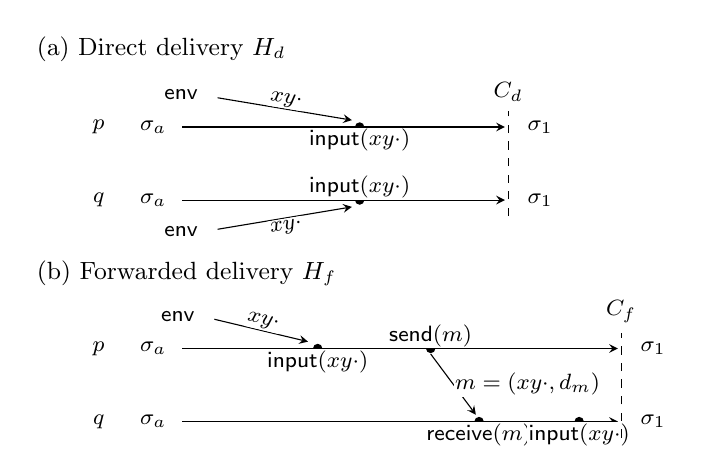
\begin{tikzpicture}[x=.82cm,y=.58cm,>=stealth,
                      every node/.style={font=\footnotesize}]
    
    \node[anchor=west,font=\small] at (-1,7.2) {(a) Direct delivery $H_d$};
    \node[anchor=east] at (.35,5.5) {$p$};
    \node[anchor=east] at (.35,3.9) {$q$};
    \node[anchor=west] at (.6,5.5) {$\sigma_a$};
    \node[anchor=west] at (.6,3.9) {$\sigma_a$};
    \draw[->] (1.4,5.5) -- (6.4,5.5);
    \draw[->] (1.4,3.9) -- (6.4,3.9);
    \fill (4.15,5.5) circle (1.7pt);
    \fill (4.15,3.9) circle (1.7pt);
    \node[below,fill=white,inner sep=.5pt] at (4.15,5.5)
      {$\mathsf{input}(xy\cdot)$};
    \node[above,fill=white,inner sep=.5pt] at (4.15,3.9)
      {$\mathsf{input}(xy\cdot)$};
    \node[anchor=east] at (1.8,6.2) {$\mathsf{env}$};
    \node[anchor=east] at (1.8,3.2) {$\mathsf{env}$};
      \draw[->] (1.95,6.14) -- node[midway,above,sloped,fill=white,inner sep=.5pt]
        {$xy\cdot$} (4.03,5.65);
      \draw[->] (1.95,3.26) -- node[midway,below,sloped,fill=white,inner sep=.5pt]
        {$xy\cdot$} (4.03,3.75);
    \draw[dashed] (6.45,3.55) -- (6.45,5.85);
    \node[above] at (6.45,5.85) {$C_d$};
    \node[anchor=west] at (6.6,5.5) {$\sigma_1$};
    \node[anchor=west] at (6.6,3.9) {$\sigma_1$};

    
    \node[anchor=west,font=\small] at (-1,2.3) {(b) Forwarded delivery $H_f$};
    \node[anchor=east] at (.35,.65) {$p$};
    \node[anchor=east] at (.35,-.95) {$q$};
    \node[anchor=west] at (.6,.65) {$\sigma_a$};
    \node[anchor=west] at (.6,-.95) {$\sigma_a$};
    \draw[->] (1.4,.65) -- (8.15,.65);
    \draw[->] (1.4,-.95) -- (8.15,-.95);
    \node[anchor=east] at (1.75,1.35) {$\mathsf{env}$};
      \draw[->] (1.9,1.29) -- node[midway,above,sloped,fill=white,inner sep=.5pt]
        {$xy\cdot$} (3.35,.8);
    \fill (3.5,.65) circle (1.7pt);
    \node[below,fill=white,inner sep=.5pt] at (3.5,.65)
      {$\mathsf{input}(xy\cdot)$};
    \fill (5.25,.65) circle (1.7pt);
    \node[above,fill=white,inner sep=.5pt] at (5.25,.65)
      {$\mathsf{send}(m)$};
    \fill (6.0,-.95) circle (1.7pt);
    \node[below,fill=white,inner sep=.5pt] at (6.0,-.95)
      {$\mathsf{receive}(m)$};
    \draw[->] (5.25,.53) -- node[midway,right,fill=white,inner sep=.5pt]
      {$m=(xy\cdot,d_m)$} (5.95,-.8);
    \fill (7.55,-.95) circle (1.7pt);
    \node[below,fill=white,inner sep=.5pt] at (7.55,-.95)
      {$\mathsf{input}(xy\cdot)$};
    \draw[dashed] (8.2,-1.3) -- (8.2,1.0);
    \node[above] at (8.2,1.0) {$C_f$};
    \node[anchor=west] at (8.35,.65) {$\sigma_1$};
    \node[anchor=west] at (8.35,-.95) {$\sigma_1$};
  \end{tikzpicture}
  \caption{Two histories from $\sigma_a=\sigma_S(x\cdot\cdot)=(x\cdot\cdot,R_0)$ to
  $\sigma_1=(xy\cdot,R_1)$, with $R_0$ and $R_1$ the tables of
  Figure~\ref{fig:election-frames}(a) and~(b).  In (a) each participant records
  $\mathsf{input}(xy\cdot)$ directly; in (b) $q$ records it after receiving $m$.  Dashed lines are consistent cuts.}
  \label{fig:participant-runs}
\end{figure}

In Figure~\ref{fig:participant-runs}, the input $xy\cdot$ reaches $q$
directly or through a message from $p$. The histories differ, but at either
cut each participant run is $\mathsf{input}(xy\cdot)$, so both endpoints are
$(\sigma_1,\sigma_1)$.

\subsection{Distributed consistency}
\label{sec:distributed-consistency}

A \emph{continuation} of a history at a consistent cut $C$ is a history $H'$
that extends the history events of $C$ with further history events after
them. All of $H'$ is a consistent cut of $H'$, its \emph{final cut}. A
consistent cut $C$ is \emph{confluent at} $j$, for a common \indesc $j$ of
the participants' current inputs, when some continuation at $C$ has a final
cut with endpoint $\bigl((j,R)\bigr)_{p\in P}$ for some $R$: every
participant ends in the same state $(j,R)$. History events at different
participants are independent, so this holds exactly when the participant runs at $C$ are
confluent at $j$ (Definition~\ref{def:consistency}).

\begin{definition}[Distributed consistency]
\label{def:distributed-consistency}
An ordered specification has \emph{distributed consistency} when, for every
finite participant set, every consistent cut of every history is confluent
at every common \indesc of the participants' current inputs.
\end{definition}

\begin{proposition}[Consistency and distributed consistency]
\label{prop:distributed-consistency}
An ordered specification is consistent if and only if it has distributed
consistency.
\end{proposition}

\begin{proof}[Proof sketch]
\textcolor{reviewed}{The participant runs at a cut are a family of runs, and any family
of runs can be placed at separate participants that exchange no messages.} Full proof in Appendix~\ref{app:proofs-sec4}.
\end{proof}

Both notions are existence claims about transitions
(Section~\ref{sec:scope}). By Complete CALM,
which reduces to Functional CALM with one output per input, a specification
has distributed consistency exactly when it satisfies Lifted Monotonicity. \textcolor{reviewed}{For functional specifications,
Corollary~\ref{cor:state-by-input} also gives convergence:}

\begin{corollary}[Convergence]
\label{cor:convergence}
In any history of a consistent functional specification, every
participant whose current input at a consistent cut is $j$ is in state
$\sigma_S(j)$. Participants with the same current input therefore agree,
regardless of message paths, arrival order, or the outputs they emitted.
\end{corollary}

\begin{proof}
Each participant run is a run; apply Corollary~\ref{cor:state-by-input}.
\end{proof}

This is the convergence that strong eventual
consistency~\cite{shapiro2011crdt} asks of replicated state---replicas that
have received the same updates are in equivalent states. \textcolor{reviewed}{The semilattice merge of CRDTs suffices for it but is not
needed: here it follows directly from any consistent functional specification.} \textcolor{reviewed}{With several outputs per input
this fails even for consistent specifications: in
Figure~\ref{fig:ambiguity-frames}(g), a run that emitted $\{s{\to}\texttt{s1}\}$
has retired the route sets that omit it, while a run at the same input that
emitted nothing keeps them.} \textcolor{reviewed}{Consistency then guarantees that such replicas can
be reconciled, not that they agree.}

\paragraph{Message data.}
The data $d$ of a message is any application state other than input that a
participant chooses to send: timestamps, version vectors, non-input-related gossip, votes, etc. Data
can influence which events occur next at the receiver, but it
never directly changes the receiver's specification state, and nothing in the
definitions above depends on it. Section~\ref{sec:systems} calls the
rule that makes these choices a participant's \emph{strategy}. Data can
influence the strategy, but the strategy can decide only within the
specification. Participants may also share emitted outputs in $d$; this does not change
which cuts are confluent (Appendix~\ref{app:exchanging-outputs}).


\subsection{Systems}
\label{sec:systems}

The histories above use the output events of
Sections~\ref{sec:functional-calm}--\ref{sec:complete-calm}, which apply
exactly the commitments an output requires: they seal the inputs in
$\Sealed_o$ and remove the rows in $\Rejected_o$
(Definition~\ref{def:output-event} and Section~\ref{sec:lifted-output-events}). Many real systems behave differently. For example, the registrar of
Section~\ref{sec:election-story} emits $\bot$ and closes the polls in the same
event (Figure~\ref{fig:election-frames}(d)); the output event for $\bot$ does
not require the poll-closing seal, so closing the polls is a design decision of
the system. Similarly, a lock manager issues a commitment to an ordering of ongoing
transactions ($A$ before $B$) without emitting that ordering until later
(Figure~\ref{fig:cc-commitments}(h) below); whether that commitment needs
coordination depends on who else may order the same transactions
(Section~\ref{sec:coordination}). \textcolor{reviewed}{We model such systems by letting them
bring bespoke commitments.}

\begin{definition}[Commitment]
\label{def:commitment}
A \emph{commitment} is a partial function on
specification states that leaves the current input unchanged and removes a
nonempty set of rows, each with no remaining row at the same input that
\outrel it: whenever $c(i,R)=(i,R')$, we have $R'\subsetneq R$ and
\begin{equation}
  (k,u)\in R\setminus R',\ (k,w)\in R'
  \quad\Longrightarrow\quad
  u\not\OutputOrd w.
  \label{eq:commitment-excludes}
\end{equation}
\end{definition}

The seals and choices of Definition~\ref{def:output-event}
and Section~\ref{sec:lifted-output-events} satisfy this definition: a seal removes
every row at the inputs it seals, and a choice removes the rows in
$\Rejected_o$. The converse also holds:

\begin{proposition}[Commitments seal inputs or choose outputs]
\label{prop:seal-or-choose}
\textcolor{reviewed}{At each input where a commitment removes rows of the state it is applied to,
it either removes every row there, \emph{sealing} that input, or removes some
outputs and keeps others, \emph{choosing} among them.}
\end{proposition}

\begin{proof}
At an input $k$, either no row remains or some does.
\end{proof}

In a functional specification each fiber has one row, so every commitment
seals. Because each commitment acts on a given state, the classification is
unambiguous. A seal may remove the last rows that earlier choices left at an
input; attributing the seal across that sequence is a provenance question we do
not pursue.

\begin{definition}[Local history, strategy]
\label{def:strategy}
A \emph{local history} of participant $p$ is a finite sequence of $p$'s history
events, including the messages it
has received. A \emph{strategy} for $p$ is a nondeterministic transition
function: it maps each local history $\lambda$ of $p$ to a set
$\theta_p(\lambda)$ of output, commitment, send, and receive events of $p$, and $p$ next
performs any one of them, or waits. Input events come from the environment,
not the strategy.
\end{definition}

\begin{definition}[System, commitment basis, produced history]
\label{def:system}
A \emph{system} consists of a \emph{commitment basis} $\mathcal B$, the set of
commitments its output and commitment events may apply, shared by all
participants, and a strategy $\theta_p$ for each participant $p$ whose output
and commitment events apply only commitments from $\mathcal B$. A distributed history \emph{produced} by the
system consists of environment inputs and events chosen by the participants'
strategies.
\end{definition}

Strategies differ by participant so we can single out replicated
systems, whose participants share one (Appendix~\ref{app:cap-response}); no
result distinguishes participants' commitments, so the basis is shared.

\begin{definition}[Output event of a system, legal output event]
\label{def:system-output-event}
Let $(i,R)$ be a state and $o\in R(i)$. An output event $\Out{\gamma}{o}$
under a basis $\mathcal B$ applies a finite, possibly empty sequence
$\gamma=c_1\cdots c_n$ of commitments from $\mathcal B$, each $c_m$ defined at
the state its predecessors leave, leaving a table $R_c$, and then retires rows
and emits $o$, all atomically; $\varepsilon$ is the empty sequence. The event
is \emph{legal} when $(i,o)\in R_c$ and every row of $R_c$ ruled out by $o$ is
\outrelpast by a retained row that \outrel $o$:
\begin{equation}
  (k,x)\in R_c\setminus R_c[\mathrm{out}\OutputGe o]
  \quad\Longrightarrow\quad
  \exists u\in R_c[\mathrm{out}\OutputGe o](k):\ x\OutputOrd u.
  \label{eq:lifted-validity}
\end{equation}
The event then retires those \outrelpast rows and ends at
$(i,R_c[\mathrm{out}\OutputGe o])$.
\end{definition}

\begin{definition}[Commitment event]
\label{def:commitment-event}
A \emph{commitment event} $\mathsf{commit}(\gamma)$ under a basis $\mathcal B$
applies a nonempty sequence $\gamma=c_1\cdots c_n$ of commitments from
$\mathcal B$, each defined at the state its predecessors leave, and emits
nothing.
\end{definition}

A commitment event lets a system decide before any output needs the decision. The environment observes nothing from it. A history a system produces may
also contain commitment events; item~3 of
Definition~\ref{def:distributed-history} and participant runs
(Definition~\ref{def:participant-run}) include them, in local order, so each
participant run is a run under $\mathcal B$.

A legal $\Out{\gamma}{o}$ issues at least the commitments of the $\mathsf{output}(o)$
of Sections~\ref{sec:functional-calm}--\ref{sec:complete-calm}: its commitments
remove the rows in $\Sealed_o$ and $\Rejected_o$
(Lemma~\ref{lem:canonical-commitment-normal-form}), and $\mathsf{output}(o)$ is
the case in which they remove exactly those. The environment observes $o$, not
$\gamma$.

\paragraph{A transactional example of bespoke commitments.}
The lock manager from the start of this section is one system; multiversion
timestamp ordering (MVTO)~\cite{bernstein1981concurrency} is another, and they
have different bases (Appendix~\ref{app:cc-bases}). Two-phase locking (2PL)
has $\mathcal B_{\mathrm{2PL}}$, made of ordering commitments
$\mathsf{order}(A,B)$ together with transactional-commit, abort, and read commitments; MVTO
has $\mathcal B_{\mathrm{MVTO}}$, made of stamp commitments $\mathsf{stamp}(A)$
together with the same transactional-commit, abort, and read commitments. The ordering
commitments are where they part: $\mathsf{order}(A,B)$ fixes $A$ before $B$ and
nothing else, which no MVTO commitment does, and $\mathsf{stamp}(B)$ places $B$
before every other transaction, which no 2PL commitment does. Figure~\ref{fig:cc-commitments} shows each at work on a three-transaction
version of the ordering fiber of Figure~\ref{fig:ambiguity-frames}(f). When
$B$ waits for a lock that $A$ holds, 2PL applies $\mathsf{order}(A,B)$, leaving
$C$'s position open (panel (h)). When MVTO gives $B$ the first timestamp, it
applies $\mathsf{stamp}(B)$, placing $B$ first (panel (i)). Both are choices:
they remove serialization orders while the input stays legal, but leave
different alternatives open. Each can be applied in a commitment event
$\mathsf{commit}(\gamma)$, as below, or as one commitment in the $\gamma$ of an
output event that later emits a full serial order, and neither is the choice
$c_o$ of Section~\ref{sec:lifted-output-events}.

\begin{figure}[t]
  \centering
  \small
  \setlength{\tabcolsep}{5pt}
  \begin{tabular}[t]{@{}l l@{}}
    \multicolumn{2}{@{}l}{(h) 2PL: $A$ locks ahead of $B$}\\
    \toprule
    $\mathrm{in}$ & $\mathrm{out}$ \\ \midrule
    $\{A,B,C\}$ & \sh{$[A,B,C]$} \\
    $\{A,B,C\}$ & \sh{$[A,C,B]$} \\
    $\{A,B,C\}$ & \sh{$[C,A,B]$} \\
    \retired{$\{A,B,C\}$} & \retired{$[B,A,C]$} \\ \strikerow
    \retired{$\{A,B,C\}$} & \retired{$[B,C,A]$} \\ \strikerow
    \retired{$\{A,B,C\}$} & \retired{$[C,B,A]$} \\ \strikerow
    \bottomrule
  \end{tabular}
  \hfill
  \begin{tabular}[t]{@{}l l@{}}
    \multicolumn{2}{@{}l}{(i) MVTO: $B$ receives the first timestamp}\\
    \toprule
    $\mathrm{in}$ & $\mathrm{out}$ \\ \midrule
    $\{A,B,C\}$ & \sh{$[B,A,C]$} \\
    $\{A,B,C\}$ & \sh{$[B,C,A]$} \\
    \retired{$\{A,B,C\}$} & \retired{$[A,B,C]$} \\ \strikerow
    \retired{$\{A,B,C\}$} & \retired{$[A,C,B]$} \\ \strikerow
    \retired{$\{A,B,C\}$} & \retired{$[C,A,B]$} \\ \strikerow
    \retired{$\{A,B,C\}$} & \retired{$[C,B,A]$} \\ \strikerow
    \bottomrule
  \end{tabular}
  \caption{Serial orders of three transactions after one commitment:
  (h) 2PL orders $A$ before $B$; (i) MVTO places $B$ first.  Only complete rows without aborts or reads
  are shown.}
  \label{fig:cc-commitments}
\end{figure}

\paragraph{Canonical runs suffice.}
We call the runs of
Sections~\ref{sec:functional-calm}--\ref{sec:complete-calm} \emph{canonical
runs}, and a \emph{run under a basis} $\mathcal B$ is one whose output and commitment
events apply only commitments from $\mathcal B$ (Definition~\ref{def:run-under-basis}). \textcolor{reviewed}{Locks, timestamps, quorums, and consensus differ in how and when they decide.} Yet every output event of any system removes at least the rows that the
canonical event for its output removes
(Lemma~\ref{lem:canonical-commitment-normal-form}), and every run under any
basis has an observably equivalent canonical run: one that accepts the same
inputs, emits the same outputs, and keeps at least the original's rows after each event; its commitment events
erase to nothing (Lemma~\ref{lem:canonical-equivalent},
Appendix~\ref{app:bases}). In the remainder of the paper we therefore judge consistency on canonical
runs. \textcolor{reviewed}{Whether a specification needs coordination thus depends on the seals and choices its outputs require, whatever mechanism makes them.}

Consider 2PL on an input of three transactions $A$, $B$, $C$ that have each
issued their operations and requested commit, where $B$ waits for a lock that
$A$ holds. When $B$ begins to wait, 2PL applies $\mathsf{order}(A,B)$ in a
commitment event, before any output, keeping only the rows that can be
completed without committing $B$ before $A$. The canonical run skips that
event, so it keeps every row, including the one completed by $[B,A,C]$. When
2PL later emits $[A,C,B]$, it applies no further commitment ordering $A$ and
$B$, and the canonical run emits the same output; both end with the same
table. The lock issued its commitment to $A$ before $B$ earlier than any
output required.

\subsection{Coordination}
\label{sec:coordination}

\textcolor{reviewed}{A commitment is a binding decision that removes behavior the specification
still permits.} \textcolor{reviewed}{Mutexes, locks, timestamps, and agreement protocols have a
common semantic effect: each implements commitments, by sealing and
choosing (Proposition~\ref{prop:seal-or-choose}).} \textcolor{reviewed}{A commitment requires coordination only when another run could contradict it,
by accepting an input it sealed or emitting an output it chose against; it
requires distributed coordination when that run is at another participant.} \textcolor{reviewed}{Running such a mechanism need not issue a commitment: closing the polls after every voter
has voted still runs the mechanism, but no ballot is left to seal, so it
removes nothing the specification still permits and applies no commitment.}

\begin{definition}[Contradicting run]
\label{def:contradicts}
\textcolor{reviewed}{Let an event of a run apply a commitment.} \textcolor{reviewed}{A run \emph{contradicts} the
commitment if it accepts an input the commitment seals, or emits an output the
commitment chooses against at the same input.}
\end{definition}

\begin{definition}[Coordination-requiring commitment, distributed coordination]
\label{def:coordination}
\textcolor{reviewed}{Let $\mathcal R$ be a set of runs: for a specification, its canonical runs;
for a system, the runs it can perform under any inputs the environment may
supply.} \textcolor{reviewed}{A commitment \emph{requires coordination} relative to $\mathcal R$
when some run in $\mathcal R$ contradicts it
(Definition~\ref{def:contradicts}).} \textcolor{reviewed}{It \emph{requires distributed
coordination} when that run is at another participant of the same history.}
\end{definition}

\begin{definition}[Coordination-free]
\label{def:coordination-free}
\textcolor{reviewed}{A run or history is \emph{coordination-free} relative to $\mathcal R$ when it
applies no commitment that requires coordination relative to $\mathcal R$.}
\end{definition}

\textcolor{reviewed}{\emph{Coordination} is any operational mechanism, such as agreement, locking,
ownership, or a single sequencer, that ensures the runs of a system make no
commitments that contradict one another.} \textcolor{reviewed}{The definition does not model such
mechanisms.} \textcolor{reviewed}{It identifies the commitments that need one; how a system can
provide it, or why it sometimes cannot, is the subject of the rest of this
section.}

\textcolor{reviewed}{Whether a commitment requires coordination depends on the set of runs: those
of a specification, or those of a system implementing it.} \textcolor{reviewed}{For a
specification, every commitment requires coordination: some canonical run
accepts each input that a commitment can seal and emits each permitted
output.} Since any family of canonical runs forms a message-free history
(Proposition~\ref{prop:distributed-consistency}), that run may be at another
participant, so the coordination it requires is also distributed. For a specification,
then, coordination-free means commitment-free: every output event is some
$\Out{\varepsilon}{o}$, which may still perform output retirements, and no
commitment event occurs. This is the sense of
Sections~\ref{sec:functional-calm}--\ref{sec:complete-calm}.

\textcolor{reviewed}{For a system, the answer depends on which runs it can perform, and here seals
and choices differ.} \textcolor{reviewed}{The environment may supply any input to any participant,
so a seal requires distributed coordination whenever another participant may receive
the sealed input, whether or not one does in the run at hand.} Closing the
polls before every voter has voted seals the remaining ballots, so it requires coordination, and distributed
coordination when another polling station may accept a late ballot. \textcolor{reviewed}{Outputs, by contrast, come only from the system's strategies, so a choice
requires coordination only when the system can perform a run that emits an
output the choice rules out, and distributed coordination when such a run is
at another participant.}

The next result explains why a commitment that requires distributed
coordination calls for exclusion: a
choice and an output it rules out, at different participants, leave states that cannot be reconciled at the current input.

\begin{proposition}[Conflicting events cannot be reconciled]
\label{thm:commitments-require-coordination}
\textcolor{reviewed}{From a state $(i,R)$, let one run perform an output or commitment event after which no
output at $i$ \outrel $x$, and let another run perform an output event that
emits $x$.} \textcolor{reviewed}{The two resulting states cannot be brought to a common state with
current input $i$.}
\end{proposition}

\begin{proof}[Proof sketch]
\textcolor{reviewed}{After the second event every output at $i$ \outrel $x$, and after
the first none does; since events never add rows, no row at $i$ can be common
to both.} Full proof in Appendix~\ref{app:proofs-sec4}.
\end{proof}

The conflict is confined to the current input. If $i\InputOrd j$,
$\fiber{i}=\{o,x\}$ with $o$ and $x$ incomparable, and $\fiber{j}=\{u\}$ with
$u$ \outrelpart both, the two states can be reconciled once $j$ arrives. Consistency still
counts this as a failure, since it asks for confluence at the current input
too. \textcolor{reviewed}{The environment may act on what it observes, through channels the system
does not see, as in Lamport's ``anomalous behavior''~\cite{lamport1978time}, and the reconciling input need not arrive.} Consistency
therefore excludes every observable conflict, including a transient one.

The first event's commitment is a choice against $x$, and it requires
distributed coordination exactly when another participant may emit $x$. The system must
then exclude one of the two events: by a mutex or atomic instruction in shared
memory, by agreement in a distributed system, or by a rule fixed in advance,
such as assigning the choice to a single participant, so that only that
participant's runs can contradict it and no runtime agreement is needed. Seals are
similar, with input in place of output, but the environment may deliver any
input to any participant, so a seal avoids requiring distributed coordination only if no
other participant can receive the sealed input, a restriction on the
environment that our model does not make.

\paragraph{Locks in a shared-nothing database.}
\textcolor{reviewed}{Ownership changes which runs can contradict a commitment.} \textcolor{reviewed}{The three cases of
the definitions all arise in a database partitioned by key, in which each key
is owned by one participant, which manages its
locks~\cite{stonebraker1986sharednothing}.}

\emph{Local coordination.}  Ordering two transactions on one key requires
coordination: in another run $B$'s request arrives first and the key's owner
orders $B$ before $A$. But only runs at the key's owner can contradict it, so
it does not require distributed coordination.

\textcolor{reviewed}{\emph{Distributed coordination.}  A transaction that spans keys needs one
order, but each key's owner orders its part, and the owners of two keys can
order the same pair of transactions oppositely.} \textcolor{reviewed}{Each ordering then requires
distributed coordination, and the owners must agree.}

\textcolor{reviewed}{\emph{No coordination.}  Two-phase commit adds no coordination beyond the
owners' own.} \textcolor{reviewed}{Each owner's prepare is its own commitment, local coordination
as in the first case.} \textcolor{reviewed}{The unanimous vote that combines them, however,
requires no coordination at all: the coordinator's unanimity decision over a
fixed set of participants is monotone, so it issues no commitment that
requires coordination.} \textcolor{reviewed}{The coordinator does not make the
owners agree; it detects whether their local commitments already agree, and
aborts when they do not.} \textcolor{reviewed}{Two-phase commit can still block: if the coordinator fails after the owners
prepare, they must wait for its decision.} \textcolor{reviewed}{That is a loss of availability,
not a commitment that another participant could contradict.}

All three exchange messages, and a client cut off from an owner cannot get its
answer; only the second issues a commitment that a run at another participant
could contradict.

Confluence is a safety property, and reaching it is liveness
(Section~\ref{sec:scope}). Under Lifted
Monotonicity, participants at a common input $j$ can each emit a
$u\in\fiber{j}$ that \outrel everything emitted, without commitment
(Proposition~\ref{prop:exposure-boundary}); choosing $u$ by a shared
deterministic rule terminates once outputs stop.

\subsection{The Complete CAP Theorem}
\label{sec:complete-cap}

\textcolor{reviewed}{Brewer conjectured that a distributed system cannot be consistent, available,
and partition tolerant at once~\cite{brewer2000towards}; Gilbert and Lynch
proved it for a linearizable register~\cite{gilbert2002cap}.} \textcolor{reviewed}{Their theorem
concerns one guarantee, not which guarantees can stay available and
consistent through a partition.} \textcolor{reviewed}{Complete CAP answers that broader question for any declared guarantee.} \textcolor{reviewed}{A
guarantee is encoded as an ordered specification together with a designated
subset $E$ of its rows: those whose outputs must stay available.} \textcolor{reviewed}{This
separates what participants must be able to emit from what may be observed.} \textcolor{reviewed}{Outputs of $E$ are \emph{explicit}: some participant must be able to emit them
on its own.} \textcolor{reviewed}{The other permitted outputs are \emph{implicit}: none need ever be
emitted, but an observer outside the system may collect outputs from every
side, and the specification decides whether that collection is permitted.} \textcolor{reviewed}{Complete CAP says that such a guarantee can be
kept available and consistent through partitions exactly when the
specification satisfies Lifted Monotonicity for $E$: explicit outputs emitted
on different sides of a partition must have a common \outnoun in the
specification at every common \indesc of their inputs.} \textcolor{reviewed}{When $E$ is every permitted row, this is Lifted
Monotonicity itself.} \textcolor{reviewed}{A partition does not
change which commitments a specification needs; it removes the ability to make
them jointly, since separated participants cannot agree to seal
an input or make a choice that another could contradict.}

\begin{definition}[Partitioned history]
\label{def:partitioned-history}
\textcolor{reviewed}{A \emph{partitioned history} divides the participants into two or more
components and contains no receive whose matching send lies in another
component; participants still receive environment input and emit outputs.}
\end{definition}

\textcolor{reviewed}{We fix a system, with a strategy for each participant of every finite
participant set and every choice of initial inputs, each depending only on its
participant's local history, and an adversarial environment that may supply
any legal input event to any participant.}

\begin{definition}[Explicit relation, Availability]
\label{def:partition-notions}
\textcolor{reviewed}{A continuation of a partitioned history is \emph{local to} a participant $p$
when the system produces it, it adds only events of $p$'s component and no
input events, and none of its receives takes a message sent from another
component.} \textcolor{reviewed}{An \emph{explicit relation} $E\subseteq S$ is a set of rows
$(i,o)$ whose output $o$ must stay available at input $i$; write $E(i)$ for
its fiber $\{o:(i,o)\in E\}$.} \textcolor{reviewed}{The system has \emph{Availability for $E$}
when, in every partitioned history it produces, each participant $p$, ending
in state $(i,R)$, can emit each output in $R(i)\cap E(i)$ in some continuation
local to $p$.} \textcolor{reviewed}{\emph{Availability} is Availability for $S$.}
\end{definition}

\begin{definition}[Partition Consistency]
\label{def:partition-consistency}
\textcolor{reviewed}{The system has \emph{Partition Consistency} when the final cut of every
partitioned history it produces is confluent at every common \indesc of the
participants' current inputs.} \textcolor{reviewed}{The continuation that confluence asks for need
not stay partitioned and need not be produced by the system.}
\end{definition}

\begin{definition}[Lifted Monotonicity for $E$]
\label{def:lm-for-A}
\textcolor{reviewed}{$\Spec$ satisfies \emph{Lifted Monotonicity for $E$} when every finite set of rows of $E$ with
a common \indesc $j$ has a common \outnoun in $\fiber{j}$.}
\end{definition}

\textcolor{reviewed}{With $E=S$, Lifted Monotonicity for $E$ is the common-\indesc condition
(Definition~\ref{def:common-expansion-condition}).} Unlike Availability,
Availability for a smaller $E$ can be met by a system whose output events issue commitments without coordination, as the remark after Corollary~\ref{cor:complete-cap-S} explains.

\begin{theorem}[Complete CAP]
\label{thm:complete-cap}
\textcolor{reviewed}{For an ordered specification $\Spec$ and an explicit relation
$E\subseteq S$, the following are equivalent:}
\begin{enumerate}
\item
\textcolor{reviewed}{some system has Availability for $E$ and Partition Consistency;}
\item
\textcolor{reviewed}{$\Spec$ satisfies Lifted Monotonicity for $E$.}
\end{enumerate}
\end{theorem}

\begin{proof}[Proof sketch]
\textcolor{reviewed}{Consider the system whose strategies emit each output of
$E$ by the canonical output event of Section~\ref{sec:complete-calm}.} \textcolor{reviewed}{It has
Availability for $E$, and Lifted Monotonicity for $E$ gives the outputs it emits a
common \outnoun at every common \indesc of their inputs.} \textcolor{reviewed}{Conversely, given one
participant per row of $E$, each in its own component, Availability lets each
emit its row's output, and Partition Consistency then supplies the common
\outnoun.} Full proof in Appendix~\ref{app:proofs-sec4}.
\end{proof}

\begin{corollary}
\label{cor:complete-cap-S}
\textcolor{reviewed}{Some system has Availability and Partition Consistency if and only if $\Spec$
satisfies Lifted Monotonicity.} \textcolor{reviewed}{When it does, a commitment-free system has
both: one whose strategies may emit any exposable output $o$ with no
commitment, by $\Out{\varepsilon}{o}$.}
\end{corollary}

\begin{proof}[Proof sketch]
With $E=S$, Lifted Monotonicity for $E$ is Lifted Monotonicity itself, and the
exposure boundary makes every
output of the commitment-free system available. Full proof in Appendix~\ref{app:proofs-sec4}.
\end{proof}

A system might hope to keep more outputs available by issuing commitments,
coordinating within each side of a partition. It cannot: the impossibility
direction of the proof holds for every system, commitment-free or not. Nor
does the system in the proof need coordination. \textcolor{reviewed}{Under Lifted Monotonicity for
$E$, the canonical event
for an explicit output seals nothing and chooses only against implicit
outputs, which the system never emits, so it is
coordination-free (Definition~\ref{def:coordination-free}).} \textcolor{reviewed}{For $E=S$ it needs no
commitment at all.} For a smaller $E$ such local choices can be necessary: if
$o\in E(i)$ and $x\in\fiber{i}\setminus E(i)$ have no common \outnoun at $i$,
emitting $o$ must choose against $x$. \textcolor{reviewed}{When Lifted Monotonicity for $E$ fails, some
output of $E$ waits for another component, sacrificing Availability, or is emitted anyway, sacrificing Partition Consistency.}

\paragraph{Gilbert and Lynch.}
\textcolor{reviewed}{Their theorem is a case of Complete CAP.} \textcolor{reviewed}{Consider a register specification
whose inputs are sets of operations with their real-time precedence, and whose
outputs answer every operation of the input as some linearization
does~\cite{herlihy1990linearizability}.} \textcolor{reviewed}{Let $p$'s input contain only a write
of $v\neq v_0$, and $q$'s only a read.} \textcolor{reviewed}{The fiber at $p$'s input holds only the
write's acknowledgment; the fiber at $q$'s input, which contains no write,
holds only the answer $v_0$ to the read.} \textcolor{reviewed}{At the common \indesc where the write
precedes the read, every output in the fiber answers that same read with $v$.} \textcolor{reviewed}{That contradicts
the answer $v_0$; it is not a later read observing a newer value.} \textcolor{reviewed}{So no output
there \outrel $v_0$, and $\Spec$ does not satisfy Lifted Monotonicity.}

\textcolor{reviewed}{By Complete CAP, then, no system keeps both outputs available and consistent across a partition, which is Gilbert and Lynch's theorem.} The proof needs less than the full hypotheses here, which
is why it yields Gilbert and Lynch's theorem exactly. Place $p$ and $q$ in
separate components. Availability is used only to make $p$ acknowledge the
write and $q$ answer the read; each fiber holds a single output, so any
response will do, which is Gilbert and Lynch's availability. Partition
Consistency is used only to demand a common \outnoun of those two answers, a
single linearization that explains both, which is Gilbert and Lynch's
consistency. No such \outnoun exists.

Appendix~\ref{app:cap-response} takes precedence from real time, extends
Complete CAP to systems that choose their responses when responses are not
forced, and derives
the theorem in Gilbert and Lynch's asynchronous model.


\section{Composition and Proper Coordination}
\label{sec:composition}

\textcolor{reviewed}{Coordination poses a puzzle.} \textcolor{reviewed}{A non-monotone program needs coordination, yet
coordination is itself non-monotone.} \textcolor{reviewed}{A key-value store with mutable keys is
non-monotone~\cite{alvaro2011bloom}.} \textcolor{reviewed}{State-machine
replication~\cite{schneider1990smr} wraps it in a log.} \textcolor{reviewed}{Clients send requests,
the log puts the requested commands in one order, and the key-value store
executes the log and answers each request.} \textcolor{reviewed}{The log's specification is also not
monotone: when two commands arrive concurrently, either may be appended next,
and the two alternative orders have no common \outnoun.} \textcolor{reviewed}{Yet replicated stores are consistent, coordinating only in the log.} \textcolor{reviewed}{Multi-Paxos agrees on each
log entry~\cite{lamport2001paxos}, and the replicas then execute the agreed log
with no further agreement.}

\textcolor{reviewed}{That puzzle is explained by our framework.} \textcolor{reviewed}{Specifications are
tables, so they compose by equijoin, and composition preserves Lifted
Monotonicity.} \textcolor{reviewed}{Because commitments are explicit, we
can also ask which component makes a composition's commitments.} \textcolor{reviewed}{When the
upstream component makes every commitment the composition needs, and the
downstream needs none on the inputs the upstream offers, we call the
coordination \emph{proper}
(Section~\ref{sec:proper-coordination}).} Proofs are in
Appendix~\ref{app:composition}.
\label{sec:sequential-composition}

\textcolor{reviewed}{Intuitively, sequential composition feeds the output of one specification to
the input of the next.} \textcolor{reviewed}{The composite is again a table: it pairs an input of
the first specification with every output that the second permits for some
intermediate value that the first permits.} \textcolor{reviewed}{Formally, let
$\Spec_1=(I,\InputOrd,M,\preceq_M,S_1)$ and
$\Spec_2=(M,\preceq_M,O,\OutputOrd,S_2)$ be ordered relational specifications
sharing the ordered domain $(M,\preceq_M)$.} \textcolor{reviewed}{Their \emph{sequential
composition} has table}
\begin{equation}
  S_2\circ S_1
  =\pi_{I,O}(S_1\Join_M S_2)
  =\{(i,o):\exists m.\ (i,m)\in S_1\land(m,o)\in S_2\},
  \label{eq:spec-composition}
\end{equation}
\textcolor{reviewed}{where $\pi$ and $\Join$ are relational projection and equijoin.} \textcolor{reviewed}{Since $S_1$
is total on $I$ and $S_2$ is total on $M$ (it has a row at every $m\in M$),
every $i\in I$ has a nonempty fiber in $S_2\circ S_1$.} \textcolor{reviewed}{When the two stages
run as a pipeline, $\Spec_2$ takes the outputs of $\Spec_1$ as its inputs, and
we say that $\Spec_1$ \emph{guards} $\Spec_2$.} Appendix~\ref{sec:parameterized-composition} gives each stage an input of its
own as well, as when a store serves reads that bypass the log
(Example~\ref{ex:bare-reads}).

\begin{lemma}[Composition]
\label{lem:composition}
\textcolor{reviewed}{If $\Spec_1$ and $\Spec_2$ satisfy Lifted Monotonicity, then so does the ordered specification with table $S_2\circ S_1$.}
\end{lemma}

\begin{proof}[Proof sketch]
\textcolor{reviewed}{Take rows of $S_2\circ S_1$ whose inputs have a common \indesc $j$.} \textcolor{reviewed}{The
common-\indesc condition for $\Spec_1$ gives an intermediate value at $j$ that \outrel each row's, and that value is a common \indesc
at which the condition for $\Spec_2$ supplies the common \outnoun.} Full proof
in Appendix~\ref{app:composition}.
\end{proof}

\textcolor{reviewed}{By associativity the lemma extends to finite pipelines.} For a function $f$,
its table $\{(i,f(i))\}$ satisfies Lifted Monotonicity exactly when $f$ is
monotone (Section~\ref{sec:lifted-monotonicity}).

\subsection{Composite CALM}
\label{sec:composite-calm}

The composite is itself an ordered specification. By Complete CALM, specification $S_2\circ S_1$ is consistent exactly when it
satisfies Lifted Monotonicity, and then no output needs a commitment
(Theorem~\ref{thm:complete-calm}, Proposition~\ref{prop:exposure-boundary}). \textcolor{reviewed}{That test treats the composite as a single specification.} \textcolor{reviewed}{Suppose instead that
each stage runs on its own, with its runs taking as input the outputs of the
stage before.} \textcolor{reviewed}{A stage may then need a commitment even when the composite
needs none.} \textcolor{reviewed}{A composite can be jointly monotone, with no stage needing a
commitment, in three ways.} The orders on $I$ and $O$ are part of the composite's contract
with its environment. The order on $M$ is not: the composite's table never
mentions it, and some order on $M$ may make both stages monotone.

First, every stage is monotone. By Lemma~\ref{lem:composition} the pipeline
is monotone, and no stage need make a commitment (Corollary~\ref{cor:pipelines}). The CRDT observations of Section~\ref{sec:crdt-instance} have this shape: a
client query $q$ over the replica state $s$ is the composition $q\circ s$, and
compositions of monotone functions are monotone
(Corollary~\ref{cor:functional-composition}), so
monotonicity of $q$ on all of the state domain suffices.

Second, the upstream can filter out the inputs on which the downstream is not
monotone. Consider a counter capped at $9$ that feeds a test of whether the
count is below $10$. With counts ordered numerically and the answers yes and
no incomparable, the test is not monotone: it answers yes at $0$ through $9$
and no at $10$. But the counter never produces $10$ or higher. The
downstream need only be monotone on the values the upstream can produce.

Third, considering a different order on $M$ can make two
non-monotone stages both monotone. Order the booleans with false below
true for $I$, $O$ and $M$. Consider a double-toggle: two stages that
each negate a boolean compose to the identity. Neither is monotone, but under the reversed order on
$M$, both are (Appendix~\ref{app:composition}).

We say that $S_2$ satisfies Lifted Monotonicity \emph{on} a set $D\subseteq M$
when its restriction to inputs in $D$ does.

\begin{proposition}[Jointly monotone composites]
\label{prop:joint-monotone}
The composite $S_2\circ S_1$ satisfies Lifted Monotonicity, and so is
consistent and needs no commitment, in each of the following cases.
\begin{enumerate}
\item
$\Spec_1$ and $\Spec_2$ satisfy Lifted Monotonicity.
\item
$\Spec_1$ satisfies Lifted Monotonicity; $\Spec_2$ satisfies it on
        $\Spec_1$'s outputs.
\item
$\Spec_1$ and $\Spec_2$ satisfy Lifted Monotonicity via a different order
        on $M$.
\end{enumerate}
\end{proposition}

\begin{proof}[Proof sketch]
(1) is Lemma~\ref{lem:composition}. (2) The proof of the lemma uses only
intermediate values in fibers of $\Spec_1$. (3) The composite joins the two
tables on the intermediate value and never compares two of them, so its table
is the same under a different order. Apply the lemma under that order. Full
proof in Appendix~\ref{app:composition}.
\end{proof}

The three cases do not cover every monotone composite
(Appendix~\ref{app:composition}). \textcolor{reviewed}{When no case applies, some stage may have to issue a commitment even though the composite is monotone.}

\subsection{Proper Coordination}
\label{sec:proper-coordination}

The replicated store of the opening extends the filtering case of
Proposition~\ref{prop:joint-monotone}(2). \textcolor{reviewed}{The key-value store is not monotone
on its own, but it is monotone on what the log offers: a log fixes the order
of commands, and a longer log only extends the responses.} \textcolor{reviewed}{Unlike the
filtering case, the upstream must issue a commitment to offer only such inputs.}

\textcolor{reviewed}{Let $\Spec_1$, which guards $\Spec_2$, be run by a system with any basis, and
let $\Spec_2$ run under a system of its own.} \textcolor{reviewed}{Write $\Spec_2|_{\Spec_1}$ for $\Spec_2$ restricted to the outputs of
$\Spec_1$.}

\begin{definition}[Proper Coordination]
\label{def:proper-coordination}
\textcolor{reviewed}{A pipeline in which $\Spec_1$ guards $\Spec_2$ is \emph{proper} when
$\Spec_2|_{\Spec_1}$ needs no commitment: every output at every state it
reaches without commitment is exposable.}
\end{definition}

\begin{theorem}[Proper Coordination]
\label{thm:proper-coordination}
\textcolor{reviewed}{Fix any system for $\Spec_1$.}
\begin{enumerate}
\item
The pipeline is proper exactly when $\Spec_2$ satisfies Lifted
        Monotonicity on the outputs of $\Spec_1$.
\item
\textcolor{reviewed}{If it is proper, $\Spec_2|_{\Spec_1}$ under the empty basis follows
        every run of $\Spec_1$.} \textcolor{reviewed}{The result is a run of $S_2\circ S_1$, and
        whenever runs of $\Spec_1$ can be brought to a common state, the
        composite runs are confluent.}
\item
\textcolor{reviewed}{If it is proper and $S_2\circ S_1$ violates Lifted Monotonicity,
        $\Spec_1$ cannot emit some output without a commitment.}
\end{enumerate}
\end{theorem}

\begin{proof}[Proof sketch]
\textcolor{reviewed}{(1) is Complete CALM and the exposure boundary
(Theorem~\ref{thm:complete-calm}, Proposition~\ref{prop:exposure-boundary})
applied to $\Spec_2|_{\Spec_1}$.} \textcolor{reviewed}{(2) Each output event of $\Spec_1$ keeps
only rows above its output, so each input $\Spec_2$ receives lies above the
previous one, and by (1) every answer is exposable.} \textcolor{reviewed}{(3) The exposure boundary
of the composite fails at a canonical state, which is the image of a canonical
state of $\Spec_1$.} Full proof in Appendix~\ref{app:composition}.
\end{proof}

\textcolor{reviewed}{The theorem holds whatever basis $\Spec_1$ uses, and a proper pipeline is
itself a guard for a further stage (Corollary~\ref{cor:pipelines}).} \textcolor{reviewed}{Locks in
the key-value store would be pure overhead: by (1), the store restricted to
logs needs no commitment.}

Sequential composition, products of independent stages, and glue stages that
copy, merge, or route outputs build arbitrary acyclic graphs. A graph
satisfies Lifted Monotonicity when every node does on the outputs offered to
it, checked node by node much as types are
(Appendix~\ref{app:dataflow-graphs}).

\section{Related Work and Mappings}
\label{sec:instances}
\label{sec:related}

\textcolor{reviewed}{Complete CALM provides a unified lens for many results across literatures.} \textcolor{reviewed}{For the key related ideas, we provide mappings here to our specification model.} \textcolor{reviewed}{Each setting declares an input, an output, and their orders before
applying either CALM theorem.}

\subsection{Query monotonicity}
\label{sec:query-instance}

\textcolor{reviewed}{As previously discussed (\S\ref{sec:functional-calm}),
the CALM Theorem of Ameloot et al.\ proves an operational result for
relational languages on transducer networks: coordination-free evaluation is possible
iff a program is monotone,
under its data-placement and execution assumptions~\cite{ameloot2013relational,ameloot2015weaker}.} \textcolor{reviewed}{Functional CALM does not replace the details of that theorem.} \textcolor{reviewed}{It abstracts
the result to a property that can be compared with specifications outside
Datalog.}

\textcolor{reviewed}{Subsequent extensions to the original CALM Theorem become changes to the input
domain and its order, or to the notion of coordination.} Zinn et al.\ gave transducers partial knowledge of how data is
placed, and more queries became coordination-free, among them the
non-monotone win-move query~\cite{zinn2012winmove}. Ameloot et al.\
characterized the new classes by weaker forms of
monotonicity~\cite{ameloot2015weaker}, correcting an earlier one-fact
version~\cite{zinn2012weak}. A query is \emph{domain-distinct-monotone} when
$Q(I)\subseteq Q(I\cup J)$ for every $J$ whose facts each contain a value
that does not occur in $I$. It is \emph{domain-disjoint-monotone} when this
holds for every $J$ whose facts use only such values. Each is Functional
CALM under a different input order. Under policy-aware placement, a node can
learn which facts over its known values are absent, so the input it cannot
yet rule out is a domain-distinct $J$. Under domain-guided placement it is a
domain-disjoint $J$. When the order lets $I\cup J$ \inrelbase $I$ only for
such $J$, each condition is functional monotonicity. \textcolor{reviewed}{Functional CALM takes
the order as given.}

Baccaert and Ketsman's \emph{behaviors} map located input facts to sets of
permitted located outputs~\cite{baccaert2023dcbq,baccaert2026spectrum}. Under
inclusion of outputs, with inputs \inrelpart only by facts at new nodes, a
behavior is a relational specification. A transducer computes a behavior if
every fair run ends at a permitted output, and so implements a sub-behavior
$A$. A list of all nodes lets nodes wait for everyone and choose
consistently. Without it, isolated nodes may be the whole network and must
emit. Their characterization, \emph{node monotonicity} of $A$, is the
common-\indesc condition on $A$ for two rows at disjoint networks. Complete
CAP extends it to overlapping networks, since Availability lets no participant
wait. Delays are finite, so their construction waits: a group's smallest node
chooses once every member confirms the group. Groups sharing a node are
nested, so the choice requires coordination, but not distributed coordination
(Definition~\ref{def:coordination}). Pairing off nodes, leaving at most one
unpaired, is node monotone, yet every $A$ pairs $b$ with $a$ at $\{a,b\}$ and
with $c$ at $\{b,c\}$. For deterministic behaviors the two conditions
coincide.

\subsection{CRDTs: monotone queries over convergent state}
\label{sec:crdt-instance}

A CRDT guarantees that replicas receiving the same updates converge to
equivalent states, whatever the order of delivery and merge. But the Strong
Eventual Consistency property it offers provides no guarantee on what the
environment may observe, and is subject to Lamport's ``anomalous
behavior''~\cite{lamport1978time} (\S\ref{sec:coordination}). \textcolor{reviewed}{Laddad et al.\
proposed monotonicity as the right test for safe observation from CRDT
state~\cite{laddad2022keep}.} Their example is a two-phase set, whose state
$(\mathit{Add},\mathit{Del})$ merges by componentwise union. The query
$\mathit{Add}\setminus\mathit{Del}$ can expose added items that are subsequently
deleted. \textcolor{reviewed}{We make the proposed test precise with Functional CALM.}

\textcolor{reviewed}{Let $(D,\sqsubseteq,\sqcup)$ be the state join-semilattice.} \textcolor{reviewed}{The input is the
finite set $U$ of immutable payloads received so far, ordered by inclusion, and
the replica's state is $s(U)=s_0\sqcup\bigsqcup U$.} Then $U\subseteq V$
implies $s(U)\sqsubseteq s(V)$, and $s(U_1)\sqcup s(U_2)=s(U_1\cup U_2)$ is the
least state \outrelpart both~\cite{shapiro2011crdt}. \textcolor{reviewed}{A client observation
$q:D\to(Y,\preceq_Y)$ gives the client-visible specification $q\circ s$.} \textcolor{reviewed}{By
Functional CALM, $q\circ s$ is consistent exactly when $U\subseteq V$ implies
$q(s(U))\preceq_Y q(s(V))$.} \textcolor{reviewed}{Monotonicity of $q$ on all of $D$ suffices, but
$q$ need only be monotone between reachable states.} \textcolor{reviewed}{The query $\mathit{Add}\setminus\mathit{Del}$ over a two-phase set fails the test: a deleted item grows $U$ and shrinks the answer.} Operation-based CRDTs fit too, with the causally closed set of
delivered operations as
input~\cite{shapiro2011crdt,burckhardt2014replicated,baquero2014operation,hellerstein2025turtles}.

\textcolor{reviewed}{CRDT states form a join-semilattice, but $q$ needs less:
Complete CALM requires only \emph{some} common \outnoun of query outputs
(Section~\ref{sec:lifted-monotonicity}), not a least one.}

\subsection{Highly available transactions}
\label{sec:hat-instance}

Bailis et al.\ define isolation levels by Adya's phenomena, adding sessions and
per-item dependencies, and give highly available algorithms for the weaker
levels~\cite{bailis2013hat,adya1999weakconsistency}. We take their
assumptions as given. Items are partially replicated, and a client sends each
operation to some replica of its item. A transaction's writes carry a unique
client timestamp, and versions are ordered by timestamp, last writer wins. The system never aborts a transaction on its own. A replica answers a read
with the highest-timestamped committed write of the item that it has received.

\begin{definition}[HAT specification]
\label{def:hat-spec}
\textcolor{reviewed}{An input is a history of received events ordered by happens-before: reads,
each tagged with its replica; commits, each with its client timestamp and
write set; and deliveries of committed writes to replicas.} Events follow
each client's program order and each replica's arrival order, and a
transaction's reads precede its commit, which precedes its deliveries. Inputs are ordered by downward-closed extension. An output is a set of read
answers, ordered by inclusion. For an isolation level $L$, $S_L$ permits an
output at an input when it extends to a history that answers every read,
orders versions by timestamp, and exhibits none of the phenomena that $L$
proscribes. \textcolor{reviewed}{The explicit relation $E$ holds, at each input, the answers that
the read rule above gives.}
\end{definition}

\begin{theorem}[HAT levels]
\label{thm:hat-levels}
\textcolor{reviewed}{Suppose each transaction's timestamp exceeds that of every version it reads.} \textcolor{reviewed}{For read uncommitted and read committed, $E\subseteq S_L$ and $S_L$
satisfies Lifted Monotonicity for $E$, so by Complete CAP these levels stay
available and consistent through partitions.} \textcolor{reviewed}{For any level that proscribes
Lost Update, including snapshot isolation, repeatable read, and
serializability, no explicit relation that answers every read satisfies
Lifted Monotonicity for it.}
\end{theorem}

\begin{proof}[Proof sketch]
A read's answer under $E$ depends only on the events that precede it, so
later input never changes it, and the timestamp condition rules out the
dependency cycles of G0 and G1c. For the converse, let two transactions at
different replicas each read $x_0$ and write $x$. Each replica's answer is
forced, and their union contains a cycle on $x$ with an anti-dependency,
which is Lost Update.
\end{proof}

The timestamp condition is needed. With timestamps fixed when a transaction
begins, as in the pseudocode of the extended version of Bailis et
al.~\cite{bailis2013hatextended}, a transaction that reads a version with a
higher timestamp and then overwrites it forms a G1c cycle, so read
committed's read rule is not contained in $S_L$. Taking the timestamp at
commit, above every version read, removes the cycle.

Session guarantees, which Bailis et al.\ achieve under sticky availability,
are deployments in our terms (Proposition~\ref{thm:complete-cap-deployment});
we do not treat them here.

\textcolor{reviewed}{Mahajan et al.\ showed that no consistency semantics stronger than real-time
causal consistency can be enforced in an always-available, one-way convergent
system~\cite{mahajan2011consistency}.} Their availability, that every
request is eventually answered, is a response obligation in our terms
(Appendix~\ref{app:cap-response}). Their result is a maximality claim:
real-time causal consistency is achievable, and no stronger semantics is. With real-time precedence recorded in the input, we recover both halves
(Appendix~\ref{app:rtc}). The specification is the real-time causal product
interface, in which each replica answers its own reads. It is
coordination-free, and no strict strengthening of it is, provided that the
strengthening, like their implementations, does not consult real time. One-way convergence needs no
separate assumption, since the input records which writes each replica has
received.

\subsection{Invariant confluence}
\label{sec:iconfluence-instance}

An invariant is a predicate that every state must satisfy. We follow the model
of Bailis et al.~\cite{bailis2014coordination}. A database state is a set of
versions, and replicas merge states by union. Each transaction $t\in T$ runs
on the state of the replica that executes it and adds the versions it writes,
so $t(s)\supseteq s$. An initial state $s_0$ satisfies the invariant
$\mathcal I$. A state is \emph{reachable} when it can be derived from $s_0$ by
applying transactions and merging states, with every state along the way
satisfying $\mathcal I$. Every reachable state descends from $s_0$, so $T$ is
\emph{invariant confluent} exactly when $\mathcal I(s_1\cup s_2)$ for all
reachable $s_1$ and $s_2$.

From an instance $(s_0,T,\mathcal I)$ of their model we construct a
specification $S_{\mathcal I}$ in ours as follows (Appendix~\ref{app:iconfluence}). Inputs are \emph{transaction histories}: partial orders of events, each
labeled by a transaction in $T$, where one event precedes another when the
replica running the second saw the first. Histories are ordered by extension:
$h'$ \inrel $h$ when $h$ is a downward-closed sub-order of $h'$, so $h'$ adds
events without changing what the earlier ones saw. We keep the \emph{locally
valid} histories, in which every transaction step preserves $\mathcal I$ on
its replica's state. Outputs are database states, ordered by inclusion: a
later state keeps every version of an earlier one. The specification table
permits, at input $h$, the state of any downward-closed sub-history of $h$
that is \emph{valid}: every merge of what it contains satisfies $\mathcal I$. A replica may thus hold transactions back, but whatever it exposes must be
valid together with everything it contains.

\begin{proposition}[Invariant confluence and Lifted Monotonicity]
\label{prop:iconfluence-lm}
\textcolor{reviewed}{$T$ is invariant confluent if and only if $S_{\mathcal I}$ satisfies Lifted
Monotonicity.}
\end{proposition}

\begin{proof}
See Appendix~\ref{app:iconfluence}.
\end{proof}

The uniqueness constraint of Bailis et al.'s payroll example shows the failure
directly. Two replicas each create an employee and assign ID~7, which each
sees is unused. The history in which neither creation saw the other is
locally valid and \inrel both one-creation histories, but its state has two
employees with ID~7, so no state it permits \outrel both. The system must
reserve IDs, reject one creation, or weaken the invariant. Concurrency,
not the transactions alone, decides the outcome: a transaction that is harmless
after another can, when it runs without seeing it, produce a state whose merge
with the other's is invalid.

Invariant preservation and transaction availability are different
specifications: $S_{\mathcal I}$ constrains exposed database states, while an
isolation level constrains exposed read and commit facts. Kaki et
al.~\cite{kaki2018alone} relate the two for a given program: they infer the
weakest isolation level a store offers under which each transaction still
preserves the declared invariants.

\subsection{General operational specification models}
\label{sec:operational-models}
Labeled transition systems and I/O automata provide general operational models
of components, including input, output, and internal actions, composition, and
implementation (simulation) relations~\cite{lynch1987io,lynch1996distributed}. They answer how a declared
machine may execute and how one machine implements another. Our goal is
narrower: the ordered relation and its remainder tables expose which observable
alternatives remain, which removals preserve prior information, and which are
binding commitments. Section~\ref{sec:distributed-execution} provides a projection from 
distributed histories, connecting our abstraction back to
participant-local executions and message causality. Thus our specification model
does not replace an operational formalism; it is a semantic
projection designed to make the intrinsic coordination question comparable
across such formalisms.

\paragraph{Compiling a state machine.}
\textcolor{reviewed}{Automata are a traditional way to model operational behavior
abstractly~\cite{lynch1987io,lynch1996distributed}.} \textcolor{reviewed}{Our model keeps only the
inputs and outputs of that behavior and drops the operational details.} \textcolor{reviewed}{The
mapping is straightforward: for each input, record the outputs of the runs that
consume it.} \textcolor{reviewed}{Work that models systems as state machines therefore maps
naturally into our model, where Complete CALM assesses its consistency
directly.} We now make the mapping precise, and then explain how it is used in
practice.

We take the standard I/O-automaton model~\cite{lynch1987io} of a state
machine, its clients, and the channel that carries their events. The machine
$M$ has states $Q$, an initial state $q_0$, receive transitions on event
payloads that accept every payload in every state, output transitions that
emit an output to a client and may change state, internal transitions, and an
observation $\mathrm{obs}:Q\to O$. Each of finitely many clients may send an
event with any payload at any time and receives the machine's outputs; a
channel carries events, each at most once, to the machine's input queue, which
it consumes in order, and may reorder them on the way. In an execution of the
composed automaton, \emph{happens-before} is Lamport's
order~\cite{lamport1978time}: the transitive closure of the local order at the
machine and at each client and of the edge from sending an event to receiving
it. An output of the machine is an input of the client that receives it, so a
client's later sends happen after everything the machine had received when it
emitted that output.

\begin{definition}[Input of an execution, induced specification]
\label{def:induced-specification}
The \emph{input} of a finite execution is the set of events the machine has
received, ordered by happens-before between their sends; $h\InputOrd h'$ when
$h\subseteq h'$ and the two orders agree on $h$. The specification
\emph{induced} by $M$ and its environment pairs each input that occurs with
the machine's observation at the end of every execution with that input.
\end{definition}

This is not a distributed execution in the sense of
Section~\ref{sec:distributed-execution}. The machine is a single
participant; the clients and the channel are its environment, and outputs
flow to the environment as in Section~\ref{sec:election-story}, where the
environment may use an output when choosing later input. Happens-before here
only keeps the books: it records which events each client sent after which
outputs, so the input remembers what the environment's choices depended on. Distributing the machine is then direct: the clients remain the environment,
each client's events are sent to some participant, and among participants
Section~\ref{sec:distributed-execution} applies, with the induced
specification as the specification.

\begin{proposition}[Induced specifications]
\label{prop:induced-specification}
\leavevmode
\begin{enumerate}
\item
The induced specification is an ordered specification, and the input
        of an execution only expands as the execution continues.
\item
When there is one client and its events arrive in the order it sent
        them, every input is a chain, inputs correspond to event sequences
        ordered by prefix, and the fiber at a sequence collects the
        observations of the machine's runs that receive it in order,
        interleaved with output and internal steps. If output and internal
        steps leave the state unchanged and receiving is deterministic, the
        specification is functional and consistent exactly when
        $\mathrm{obs}(q)\OutputOrd\mathrm{obs}(q')$ for every receive
        transition $q\to q'$ from a reachable state.
\item
Every observation in the fiber at $h$ is reached by a run of the
        machine that receives each event of $h$ once, interleaved with output
        and internal steps. If the channel may reorder and clients observe no
        outputs, every such run is reached, whatever the order of its
        receives.
\item
The machine's observations are confluent across its executions---for
        executions with inputs $h_1,\ldots,h_k$ and any input $h$ that occurs
        and expands each $h_r$, some execution with input $h$ ends in an
        observation that \outrel each of theirs---exactly when the induced
        specification satisfies Lifted Monotonicity.
\end{enumerate}
\end{proposition}

\begin{proof}[Proof sketch]
(1) Inclusion with agreeing orders is a partial order, every input that occurs
has a row, and extending an execution adds received events without changing
happens-before among earlier sends. (2) A single client's sends are totally
ordered, and they arrive in that order, so an input is determined by its
sequence of payloads, and the machine's steps in an execution form a run of
the machine automaton; in the special case, the claim is monotonicity along
receive transitions, and Functional CALM. (3) The machine's steps in an
execution form such a run; without outputs to clients, happens-before orders
only each client's own sends, so all sends can precede the machine's run. (4) Unfold the fiber in the
common-\indesc condition and apply Complete CALM
(Theorem~\ref{thm:complete-calm}, Proposition~\ref{prop:common-expansion-form}).
\end{proof}

The input orders events by their sends, not by their arrivals: the machine
receives events in one total order, but that order is what differs between
executions. Outputs are where the environment's reactions enter. A client
that sends after observing an output is ordered after everything that output
reflected, and the input records that dependence; what the client saw is
recorded by the run's output events, which keep only rows that \outrelbase
it.

\paragraph{Testing and proof.}
The induced specification is defined by every finite execution of the machine
and its environment. There are infinitely many such executions, so the
induced specification is a semantic object: we can reason about it, but not
list it. Two standard approaches make that reasoning practical.

The first is testing. A simulator or model checker runs the machine and its
environment on bounded inputs~\cite{misra1986des,flanagan2005dpor}; the
input/output pairs it collects form a finite specification in our model,
which can be checked for violations of Lifted Monotonicity. This is routine engineering
practice and has found serious bugs in production
systems~\cite{newcombe2015aws,zhou2021foundationdb}. Testing suits
refutation. If Lifted Monotonicity fails, finitely many executions show it:
executions with inputs $h_1,\ldots,h_k$, and a common \indesc $h$ at which no
execution's observation \outrel all of theirs. A violation found in the
finite specification is such a witness when the exploration covers every
execution with input $h$, so that its fiber there is complete. Testing cannot show that
Lifted Monotonicity holds, since that is a claim about every input.

The second is proof. Instead of computing the induced specification, a
designer writes one down. A \emph{declared} specification $D$ gives, for each
input, a set of outputs by a rule, such as ``the set of ballots received'' or
``the largest timestamp seen''; it does not enumerate executions. The proof
then shows that $D$ describes the machine well enough that Lifted Monotonicity
can be checked on $D$ instead. Two things must be shown, and both are needed,
because neither half alone preserves Lifted Monotonicity: if $D$ omits an
output the machine can produce, it may hide an incompatibility, and if $D$
adds an output the machine cannot produce, it may supply a common \outnoun
that no execution reaches.
\begin{itemize}
\item
\emph{Realizability.}  Every output that $D$ allows at an input is the
        observation of some execution with that input.
\item
\emph{Domination.}  Every execution's final observation is
        \outrelpast by some output that $D$ allows at its input.
\end{itemize}
$D$ need not match the machine exactly: it may leave out observations that
others \outrelbase, such as transient intermediate states.

\begin{proposition}[Declared specifications]
\label{prop:declared-specification}
Let $D$ be an ordered specification whose inputs correspond, by an order
isomorphism, to the inputs that occur. If $D$ satisfies realizability and
domination, then $D$ satisfies Lifted Monotonicity exactly when the induced
specification does, and so exactly when the machine's observations are
confluent across its executions.
\end{proposition}

\begin{proof}[Proof sketch]
Use the common-\indesc form. Given rows of the induced specification,
dominate each by a row of $D$, take their common \outnoun in $D$, and realize
it. Conversely, rows of $D$ are rows of the induced specification, and their
common \outnoun there is dominated back into $D$.
\end{proof}

Both obligations are standard in the verification literature. Domination
says that the machine refines $D$: every observation of every execution is
allowed by $D$, up to refinement of outputs. It is proved with an
\emph{invariant}, a property of the machine's state that holds initially, is
preserved by every step, and implies that the observation is dominated; it is
checked one step at a time, never by enumerating executions. This is the core
of refinement proofs for state machines, which Lynch and Vaandrager call a
forward simulation~\cite{lynch1995forward} and Abadi and Lamport a refinement
mapping~\cite{abadi1991refinement}; such proofs are routinely mechanized for
practical distributed systems~\cite{hawblitzel2015ironfleet}. Realizability
is the converse inclusion, that $D$ allows nothing the machine cannot produce. It too is proved once for all inputs, typically by induction on the input,
giving a uniform recipe that builds, for any declared row, an execution that
produces it. The proposition asks for nothing beyond these two facts. It
says that together they let $D$ stand in for the machine: Lifted Monotonicity
is checked on $D$ exactly as everywhere else in this paper, and nothing about
coordination is proved about the machine itself.

\subsection{Scope}
\label{sec:scope}

\textcolor{reviewed}{Our conditions are semantic.} Confluence guarantees that a common \outnoun
exists, not that a deployed system reaches it. A participant may lack the
authority to emit it (Appendix~\ref{app:deployment}), and reaching it takes an
algorithm, message delivery, and a termination argument. Participant runs
likewise set aside delivery and strategy details. Protocols,
liveness, and cost belong to the operational model in which a specification is
realized.


\section{Discussion}
\label{sec:discussion}

\textcolor{reviewed}{The computing literature is rich with coordination mechanisms for managing
concurrency within and across machines.} \textcolor{reviewed}{The CALM Conjecture asked a question
still latent at the time: when are these mechanisms required, and why?} \textcolor{reviewed}{It drew
on declarative networking~\cite{loo2009declarative}, which, in Codd's tradition
of separating specification from implementation~\cite{codd1970relational}, wrote
the desired effects of protocols as queries to be analyzed and optimized into a
variety of mechanisms.} \textcolor{reviewed}{Could a signature property of declarative
languages---monotonicity---be the criterion?}

\textcolor{reviewed}{The intuition was sharpened by a related friction in the literature on parallel
query processing.} \textcolor{reviewed}{The Google MapReduce
paper~\cite{dean2004mapreduce} departed from prior work on parallel query
processing~\cite{wilschut1991dataflow,graefe1990volcano}, conflating data
redistribution (shuffle) with barrier coordination required for a non-monotone
reduce operator.} \textcolor{reviewed}{This coupling of unrelated concerns required monotone operators
like join to block in the MapReduce model unnecessarily.} \textcolor{reviewed}{Cost models that count
rounds, from BSP supersteps to MapReduce rounds, carry the same
conflation~\cite{valiant1990bsp,karloff2010mrc}.}

\textcolor{reviewed}{The CALM Conjecture hypothesized that the database community's more judicious
use of barriers could be generalized: coordination---of any kind---is required
if and only if the program is non-monotone.} \textcolor{reviewed}{Ameloot et al.\
proved it, but only for relational languages, which to date have
still not become mainstream beyond query processing (more on this below).}

\textcolor{reviewed}{This paper moves the declarations one level higher, from queries to views: all
that matters about a specification is the single view mapping a program's inputs
to its output.} \textcolor{reviewed}{Eliding the query logic frees the analysis from any particular
language and broadens what can be specified.} \textcolor{reviewed}{Prior work focused on implementing
complex programs
declaratively~\cite{loo2005overlays,loo2009declarative,chu2007declarative,alvaro2011bloom}.} \textcolor{reviewed}{This was interesting ``declarative engineering'' with concrete benefits in
analysis and optimization.} \textcolor{reviewed}{But the higher-level model here also captures abstract
families of guarantees, like CAP and isolation levels, which have no application or
protocol in mind.}

\textcolor{reviewed}{Lifting the abstraction improves the power of analysis as well.} \textcolor{reviewed}{Prior program
analyses became enmeshed in the details of implementations, however
declarative.} \textcolor{reviewed}{Bloom~\cite{alvaro2011bloom} flagged syntactic non-monotonicity in
programs and conservatively injected coordination code in front of it.} \textcolor{reviewed}{Yet
coordination code is itself non-monotone, so adding it to a Bloom program only
adds more non-monotone syntax.} \textcolor{reviewed}{Jagannathan and colleagues moved the question
from syntax to declared contracts and
invariants~\cite{sivaramakrishnan2015quelea,kaki2018alone}.} \textcolor{reviewed}{Their tools pick,
for each operation or transaction, the weakest consistency or isolation level
that the store offers and that still satisfies the declared properties.} \textcolor{reviewed}{We
ask what the specification itself requires, independent of any menu of
levels.} \textcolor{reviewed}{Because the canonical commitments are universal
(Section~\ref{sec:systems}), the answer holds for every mechanism.} \textcolor{reviewed}{Our
composition results need no program logic, and the criteria are exact on
specifications, not conservative.}

\textcolor{reviewed}{A limitation of prior CALM work was that it was constructive on only one side of
its boundary.} \textcolor{reviewed}{Monotone programs need no coordination; for a non-monotone
program, CALM said only that coordination was required somewhere, not what it
had to accomplish or where it belonged.} \textcolor{reviewed}{Complete CALM says more.} \textcolor{reviewed}{A
specification that is not monotone needs specific commitments: the seals and
choices its outputs require.} \textcolor{reviewed}{Every coordination mechanism, from locks to
consensus, is a way of making these commitments.} \textcolor{reviewed}{The same analysis says which outputs
need commitments, and whether another participant could contradict them, so
that agreement is required and not just a local decision.} \textcolor{reviewed}{Proper coordination
then places the commitments in a composition: it identifies the stage that
must make them, as the log does in state-machine replication, and certifies
that the stages behind it need none of their own.}

\textcolor{reviewed}{Underlying these issues is a reassessment of
tradition: what is a declarative specification, and how little does it require
to be useful?} \textcolor{reviewed}{The question is timely.} \textcolor{reviewed}{Coding agents increasingly write
imperative code, often rife with bugs, which has renewed interest in formal
specification languages like Lean~\cite{demoura2021lean4}.} \textcolor{reviewed}{A higher-level
language keeps agents out of the incidental complexity of implementations and
pairs them with proofs of correctness: neurosymbolic
computing~\cite{an2025neurosymbolic}.} \textcolor{reviewed}{This is a renewed opportunity for logic,
dataflow, and functional languages.} \textcolor{reviewed}{Today these languages typically specify
protocols and programs in detail, as in declarative networking; this paper
points to specification at a higher level still, opening analyses like ours and
potential program synthesis and optimization.}

\section{Conclusion}
\label{sec:conclusion}

\textcolor{reviewed}{A specification abstracts execution details away, and the results here reduce
to a single question: can a participant act on what it knows without being
contradicted by what it learns later?} \textcolor{reviewed}{Mutexes, locks, atomic instructions, and
agreement protocols prevent such contradictions by making commitments.} \textcolor{reviewed}{Functional CALM answers the question for functions: a functional specification
stays confluent as input arrives exactly when it is monotone, and then no
output needs a seal.} \textcolor{reviewed}{This generalizes the classic result from logical fact
sets to arbitrary input and output orders.}

\textcolor{reviewed}{Complete CALM extends the answer to specifications that offer several outputs
for one input.} \textcolor{reviewed}{The test is Lifted Monotonicity, which combines Relational
Monotonicity with Directed Outputs.} \textcolor{reviewed}{When it fails, some reachable output
requires a commitment, and every commitment does one of two jobs: it seals
input or it chooses among outputs.} \textcolor{reviewed}{Because commitments are explicit, the model
can also check where a composition coordinates
(Section~\ref{sec:composition}).} \textcolor{reviewed}{For example, a totally ordered log and a
key-value store are both non-monotone at their ordinary specifications, yet
when the log guards the store, the log's commitments are all the composition
needs and the store makes none.} \textcolor{reviewed}{Multi-Paxos is one way to distribute those
commitments.}

\textcolor{reviewed}{Complete CAP is the partition form of the same equivalence.} \textcolor{reviewed}{A system can keep a guarantee's explicit outputs available, and consistent, through partitions exactly when they have a common \outnoun at every common \indesc of their inputs; when every output is explicit, this is Lifted Monotonicity.}

\textcolor{reviewed}{The generality of our specification model opens a range of new questions
regarding the ambiguity of specifications and their commitments.} \textcolor{reviewed}{One direction
extends the boolean criteria of this paper to metrics: a Determination
Complexity theory that assesses \emph{how many} commitments are intrinsically
needed to determine a specification.} \textcolor{reviewed}{Another is Determination Provenance: a
given output---or its absence---is determined not only by inputs, but also by
the commitments made in a run, which brings formal models of provenance to
concurrent systems.} \textcolor{reviewed}{A third direction is to provide general-purpose static
analysis of CALM and proper coordination in a real programming framework.}


\appendix
\section{Notation and terms}
\label{app:notation}

The table collects the paper's notation and defined terms, in the order the
sections introduce them, with a pointer to each definition.

\paragraph{Relational notation.}
To describe how execution narrows $S$, we use a compact relational notation. For any relation
$R\subseteq I\times O$, we select rows by writing a predicate on its
columns $\mathrm{in}$ and $\mathrm{out}$ in square brackets: $R[\mathrm{in}\InputGe j]$ is the table of rows
whose input \inrel $j$, $R[\mathrm{out}\OutputGe o]$ is the table of rows
whose output \outrel $o$, $R[\mathrm{in}\in K]$ is
the table containing the rows with inputs in $K$, etc. Commas separate conjuncts:
$R[\mathrm{in}\InputGe j,\ \mathrm{out}\OutputGe o]$ is the table of rows
satisfying both predicates. To project onto a single column, we write $\mathrm{in}(R)$ and
$\mathrm{out}(R)$ for the sets of inputs and outputs that appear in $R$. We say that a row $(k,u)$ is \emph{at} $k$; $R[\mathrm{in}=k]$ is the table of
rows at $k$.

{\footnotesize
\setlength{\tabcolsep}{3pt}
\renewcommand{\arraystretch}{1.15}

\noindent
\begin{tabular}{@{}p{.3\columnwidth}p{.5\columnwidth}p{.14\columnwidth}@{}}
  \toprule
  \multicolumn{3}{@{}l}{\textbf{Functional CALM (Section~\ref{sec:functional-calm})}}\\
  \midrule
  specification & $\Spec=(I,\InputOrd,O,\OutputOrd,S)$, total on $I$, one output per input; induced $f$ & Def.~\ref{def:functional-specification}\\
  \inrel; \indesc & $i\InputOrd j$: $j$ contains the input information in $i$ & Sec.~\ref{sec:functional-specifications}\\
  \outrel; \outnoun & $o\OutputOrd u$: $u$ preserves every visible claim in $o$ & Sec.~\ref{sec:functional-specifications}\\
  common \indesc; common \outnoun & an input that \inrel each; an output that \outrel each & Sec.~\ref{sec:functional-specifications}\\
  monotone (functional) & $i\InputOrd j\Rightarrow f(i)\OutputOrd f(j)$ & Def.~\ref{def:functional-monotonicity}\\
  selection; $\mathrm{in}(R)$, $\mathrm{out}(R)$ & $R[\text{predicate on }\mathrm{in},\mathrm{out}]$; inputs and outputs in $R$ & Sec.~\ref{sec:functional-specifications}\\
  row at $k$; fiber $R(k)$ & a row $(k,u)$; $\mathrm{out}(R[\mathrm{in}=k])$ & Sec.~\ref{sec:functional-specifications}\\
  upper fiber & $\mathrm{out}(R[\mathrm{in}\InputGe k])$ & Sec.~\ref{sec:functional-specifications}\\
  state $(i,R)$; legal input & current input and remainder table, every row at an \indesc of $i$; an input with a row in $R$ & Def.~\ref{def:residual-state}\\
  canonical state & $\sigma_S(i)=(i,S[\mathrm{in}\InputGe i])$ & Eq.~\ref{eq:canonical-state}\\
  input event; input retirement & $\mathsf{input}(j)$ keeps $R[\mathrm{in}\InputGe j]$; the rows it removes & Eq.~\ref{eq:input-event}\\
  output event; seal; commitment & $\mathsf{output}(o)$ keeps $R[\mathrm{out}\OutputGe o]$ and emits $o$; removing rows, it is a seal, a commitment & Def.~\ref{def:output-event}\\
  exposable & $\mathsf{output}(o)$ applies no commitment & Def.~\ref{def:exposable}\\
  determined; determination & the upper fiber has one element; reaching such a state & Sec.~\ref{sec:functional-events}\\
  run; commitment-free & finite event sequence from a canonical state; no output event issues a commitment & Def.~\ref{def:run}\\
  consistent; confluent at $j$ & every finite family of runs can reach one common state at each common \indesc $j$ & Def.~\ref{def:consistency}\\
  \bottomrule
\end{tabular}

\medskip
\noindent
\begin{tabular}{@{}p{.3\columnwidth}p{.5\columnwidth}p{.14\columnwidth}@{}}
  \toprule
  \multicolumn{3}{@{}l}{\textbf{Complete CALM (Section~\ref{sec:complete-calm})}}\\
  \midrule
  relational specification; ambiguous & $S\subseteq I\times O$ total on $I$; some fiber has several outputs & Def.~\ref{def:relational-specification}\\
  stranded output; incompatible pair & an output at $i$ with no \outnoun at some \indesc; two outputs at $i$ with no common \outnoun there & Sec.~\ref{sec:lifted-monotonicity}\\
  Relational Monotonicity & every output keeps a \outnoun as input \ingrows & Def.~\ref{def:relational-monotonicity}\\
  compatible in $F$; directed; Directed Outputs & some $u\in F$ \outrel all; every finite subset compatible; every fiber directed & Def.~\ref{def:fiber-directedness}\\
  joint lift $A\LiftedOrd B$ & every nonempty finite $X\subseteq A$ is compatible in $B$ & Eq.~\ref{eq:joint-output-order}\\
  Lifted Monotonicity & $i\InputOrd j\Rightarrow\fiber{i}\LiftedOrd\fiber{j}$ & Def.~\ref{def:lifted-monotonicity}\\
  common-\indesc condition & rows with a common \indesc $j$ have a common \outnoun in $\fiber{j}$ & Def.~\ref{def:common-expansion-condition}\\
  ruled out by $o$ & a row whose output does not \outrelbase $o$ & App.~\ref{app:lifted-output-events}\\
  $\Sealed_o$; $\Retired_o$; $\Rejected_o$ & ruled-out rows at inputs with no row \outrelpart $o$; \outrelpast by a kept row at the same input; the rest & Eq.~\ref{eq:seal-inputs}--\ref{eq:choice-removals}\\
  seal; output retirement; choice & remove $\Sealed_o$; remove $\Retired_o$, not a commitment; remove $\Rejected_o$ & Def.~\ref{def:lifted-output-event}\\
  \bottomrule
\end{tabular}

\medskip
\noindent
\begin{tabular}{@{}p{.3\columnwidth}p{.5\columnwidth}p{.14\columnwidth}@{}}
  \toprule
  \multicolumn{3}{@{}l}{\textbf{Distributed execution (Section~\ref{sec:distributed-execution})}}\\
  \midrule
  participant; message & holds a specification state; $m=(j,d)$, a cumulative input $j$ (or $\varnothing$) and other data $d$ & Sec.~\ref{sec:histories}\\
  distributed history; history event & locally ordered input, output, commitment, send, and receive events & Def.~\ref{def:distributed-history}\\
  happens-before; consistent cut & closure of local orders and send-before-receive; a set of history events closed under it & Def.~\ref{def:distributed-history}\\
  participant run; endpoint & $p$'s input, output, and commitment events at $C$; $(\sigma_p(C))_{p\in P}$ & Def.~\ref{def:participant-run}\\
  continuation; cut confluent at $j$ & a history extending $C$; some continuation brings every participant to one state $(j,R)$ & Sec.~\ref{sec:distributed-consistency}\\
  distributed consistency & every consistent cut of every history is confluent at every common \indesc & Def.~\ref{def:distributed-consistency}\\
  commitment & partial function on states removing rows, none \outrelpast by a remaining row at the same input & Def.~\ref{def:commitment}\\
  local history; strategy & $p$'s history events in order; $\theta_p(\lambda)$, the output, commitment, send, and receive events $p$ may perform next & Def.~\ref{def:strategy}\\
    system; basis; produced & a commitment basis $\mathcal B$ and a strategy per participant; every non-input event permitted by its strategy and using only commitments from $\mathcal B$ & Def.~\ref{def:system}\\
  system output event $\Out{\gamma}{o}$ & applies commitments $\gamma$ from the basis, retires, emits $o$ & Def.~\ref{def:system-output-event}\\
  commitment event $\mathsf{commit}(\gamma)$ & applies a nonempty sequence $\gamma$ from the basis, emits nothing & Def.~\ref{def:commitment-event}\\
  run under a basis; canonical run & events whose commitments come from the basis; a run of Sections~\ref{sec:functional-calm}--\ref{sec:complete-calm} & Def.~\ref{def:run-under-basis}\\
  observably equivalent & same input and output events, commitments and commitment events erased; every run has a canonical one & Lem.~\ref{lem:canonical-equivalent}\\
  contradicts & accepts an input the commitment seals, or emits an output it chooses against & Def.~\ref{def:contradicts}\\
  requires (distributed) coordination & a commitment some run (at another participant) contradicts & Def.~\ref{def:coordination}\\
  coordination-free & applies no commitment that requires coordination & Def.~\ref{def:coordination-free}\\
  partitioned history; explicit relation $E$; explicit, implicit output & no message crosses components; $E\subseteq S$, the rows whose outputs must stay available; outputs of $E$, and the other permitted outputs & Defs.~\ref{def:partitioned-history}, \ref{def:partition-notions}\\
  Availability for $E$; Partition Consistency & each output of $R(i)\cap E(i)$ emittable locally; final cuts of partitioned histories confluent & Defs.~\ref{def:partition-notions}, \ref{def:partition-consistency}\\
  Lifted Monotonicity for $E$ & every finite set of rows of $E$ with a common \indesc $j$ has a common \outnoun in $\fiber{j}$ & Def.~\ref{def:lm-for-A}\\
  deployment & one explicit relation $E_p$ per participant & Def.~\ref{def:deployment}\\
    response obligation; response interface & per participant, the outputs that count as answers, upward closed within fibers; a total, self-continuing explicit relation $T\subseteq Q$ & Defs.~\ref{def:response-obligation}, \ref{def:response-interface}\\
  \bottomrule
\end{tabular}

\medskip
\noindent
\begin{tabular}{@{}p{.3\columnwidth}p{.5\columnwidth}p{.14\columnwidth}@{}}
  \toprule
  \multicolumn{3}{@{}l}{\textbf{Composition (Section~\ref{sec:composition})}}\\
  \midrule
  sequential composition $S_2\circ S_1$ & $\{(i,o):\exists m.\ (i,m)\in S_1\land(m,o)\in S_2\}$, for stages sharing $(M,\preceq_M)$ & Eq.~\ref{eq:spec-composition}\\
  $\Spec_1$ guards $\Spec_2$ & $\Spec_2$ takes the outputs of $\Spec_1$ as its inputs & Sec.~\ref{sec:sequential-composition}\\
  Lifted Monotonicity on $D$ & the common-\indesc condition for rows with inputs in $D$, at \indescs in $D$ & Sec.~\ref{sec:composite-calm}\\
  restriction $\Spec_2|_{\Spec_1}$ & $\Spec_2$ restricted to the outputs of $\Spec_1$ & Sec.~\ref{sec:proper-coordination}\\
  proper & $\Spec_2|_{\Spec_1}$ needs no commitment: every output at every state reached without commitment is exposable & Def.~\ref{def:proper-coordination}\\
  \bottomrule
\end{tabular}
}

\section{Deferred proofs}
\label{app:proofs}

\subsection{Proofs for Section~\ref{sec:functional-calm}}
\label{app:proofs-sec2}

\begin{proof}[Proof of Lemma~\ref{lem:run-residual}]
The run starts at the canonical state $\sigma_S(i_0)$, whose table is
$S[\mathrm{in}\InputGe i_0]$. Each input event $\mathsf{input}(j)$ keeps only
the rows with $\mathrm{in}\InputGe j$ (Equation~\ref{eq:input-event}), and each
output event $\mathsf{output}(o)$ keeps only the rows with
$\mathrm{out}\OutputGe o$ (Equation~\ref{eq:output-action}). The input
conditions reduce to the last one, $\mathrm{in}\InputGe i$, because each later
input is an expansion of the earlier ones. One output condition remains for each
emitted output.
\end{proof}

\begin{proof}[Proof of Proposition~\ref{prop:confluence}]
A common state with current input $j$ has a row at $j$, and since rows are
never added, that row belongs to every $R_r$. Conversely, let $(j,u)$ belong
to every $R_r$. Then $\mathsf{input}(j)$ is defined at every $(i_r,R_r)$, and
$\mathsf{output}(u)$ is defined at $(j,R_r[\mathrm{in}\InputGe j])$, since
$u\in R_r(j)$. By
Lemma~\ref{lem:run-residual}, $(j,u)\in R_r$ says that $u$ \outrel every output
emitted on run $r$. After $\mathsf{input}(j)$ and $\mathsf{output}(u)$, the
same lemma leaves exactly
$S[\mathrm{in}\InputGe j,\ \mathrm{out}\OutputGe u]$, independent of the
starting run.
\end{proof}

\begin{proof}[Proof of Theorem~\ref{thm:functional-calm}]
Every input has one row, so an output emitted at current input $k$ is $f(k)$. By Lemma~\ref{lem:run-residual}, a run ending at input $i$ keeps the
row $(j,f(j))$ at an \indesc $j$ of $i$ exactly when $f(j)$ \outrel every
output the run has emitted. By Proposition~\ref{prop:confluence}, a finite
family of runs is therefore confluent at a common \indesc $j$ exactly
when $f(j)$ \outrel every output emitted on any of them. If $f$ is monotone,
this holds, since each emitted $f(k)$ has $k\InputOrd j$. If $f$ is not
monotone, some $i\InputOrd k$ has $f(i)\not\OutputOrd f(k)$. Of two
runs from $\sigma_S(i)$, one that emits $f(i)$ no longer has the row
$(k,f(k))$, while one that accepts $\mathsf{input}(k)$ keeps it; no row at $k$
survives in both, so they are not confluent at $k$.
\end{proof}

\begin{proof}[Proof of Corollary~\ref{cor:state-by-input}]
By Functional CALM (Theorem~\ref{thm:functional-calm}), the specification is
monotone. By Lemma~\ref{lem:run-residual}, the run's remainder table is
$S[\mathrm{in}\InputGe i,\ \mathrm{out}\OutputGe o_1,\ \ldots,\
\mathrm{out}\OutputGe o_m]$, where each $o_\ell=f(i_\ell)$ for some
$i_\ell\InputOrd i$. Every row whose input \inrel $i$ has the form $(k,f(k))$ with
$i_\ell\InputOrd k$, so monotonicity gives $o_\ell\OutputOrd f(k)$, and the
output conditions remove nothing.
\end{proof}

\begin{proof}[Proof of Proposition~\ref{prop:functional-exposure-boundary}]
Suppose $f$ is monotone, and let a commitment-free run reach $(i,R)$. By Functional CALM and Corollary~\ref{cor:state-by-input},
$(i,R)=\sigma_S(i)$, so the legal $j\InputGe i$ are exactly the \indescs of
$i$, and monotonicity gives $f(i)\OutputOrd f(j)$ at each, so $f(i)$ is exposable
(Definition~\ref{def:exposable}). Conversely, if every such output is exposable, then at $\sigma_S(i)$, which the
empty run reaches, exposability of $f(i)$ gives $f(i)\OutputOrd f(j)$ for every
\indesc $j$ of $i$, so $f$ is monotone.
\end{proof}

\subsection{Proofs for Section~\ref{sec:complete-calm}}
\label{app:proofs-sec3}

\begin{proof}[Proof of Proposition~\ref{prop:common-expansion-form}]
Suppose Lifted Monotonicity, and let $(i_1,o_1),\ldots,(i_k,o_k)$ be rows
with common \indesc $j$. If $k=0$, any $u\in\fiber{j}$ will do, and since
$\Spec$ is total, $j$ appears in some row $(j,u)$. Otherwise, since $i_r\InputOrd j$, Relational Monotonicity gives, for each
$r$, a $u_r\in\fiber{j}$ with $o_r\OutputOrd u_r$. The $u_r$ all lie in the
one fiber $\fiber{j}$, which is directed, so some $u\in\fiber{j}$ \outrel
every $u_r$, hence every $o_r$. Conversely, let $i\InputOrd j$ and
$X\subseteq\fiber{i}$ be nonempty and finite. The rows $\{(i,x):x\in X\}$
have common \indesc $j$, so some $u\in\fiber{j}$ \outrel all of $X$; that is
$\fiber{i}\LiftedOrd\fiber{j}$.
\end{proof}

The survivor test and Lemma~\ref{lem:run-residual} combine into the form in
which every later argument uses them.

\begin{lemma}[Reconciliation]
\label{lem:reconciliation}
Let runs end at $(i_r,R_r)$, $r=1,\ldots,m$, let $j$ be a common \indesc of
the $i_r$, and let $X$ be the set of outputs emitted on any of them. The runs
are confluent at $j$ if and only if some $u\in\fiber{j}$ \outrel every output
in $X$.
\end{lemma}

\begin{proof}
By Lemma~\ref{lem:run-residual}, $(j,u)\in R_r$ exactly when $u\in\fiber{j}$
\outrel every output emitted on run $r$. Apply
Proposition~\ref{prop:confluence}.
\end{proof}

\begin{proof}[Proof of Theorem~\ref{thm:complete-calm}]
By Proposition~\ref{prop:common-expansion-form} it suffices to treat the
common-\indesc condition. ($\Leftarrow$) Let finitely many runs end at
$(i_r,R_r)$ with common \indesc $j$. Each output $o$ emitted on a run was
emitted at some input $i_o\InputOrd j$, so $(i_o,o)$ is a row of $S$; the
condition supplies $u\in\fiber{j}$ \outrelpart all of them, and
Lemma~\ref{lem:reconciliation} gives confluence. ($\Rightarrow$) Given rows
$(i_r,o_r)$ with common \indesc $j$, apply consistency and
Lemma~\ref{lem:reconciliation} to the runs that start at $\sigma_S(i_r)$ and
emit $o_r$; for the empty family, totality gives $\fiber{j}\neq\varnothing$.
\end{proof}

\begin{proof}[Proof of Proposition~\ref{prop:exposure-boundary}]
Suppose the common-\indesc condition holds; by Theorem~\ref{thm:complete-calm}, the
specification is consistent. Let $(i,R)$ be reached by a run (commitment-free or not), and let $o\in R(i)$, $j\InputGe i$ legal, and
$x\in R(j)$. Extend the run in two ways: by $\mathsf{output}(o)$, and by
$\mathsf{input}(j)$ followed by $\mathsf{output}(x)$. By consistency the two extended runs are confluent at $j$, so
Proposition~\ref{prop:confluence} supplies a row $(j,u)$ in both tables. Both
tables are contained in $R$, so $u\in R(j)$ \outrel $o$ and $x$, and the exposure test
(Proposition~\ref{prop:exposability}) makes $o$ exposable. Conversely, suppose every such output is exposable, and let rows
$(i_1,o_1),\ldots,(i_k,o_k)$ have common \indesc $j$. By totality pick
$u_0\in S(j)$. For $r=1,\ldots,k$ in turn, the exposure test for $o_r$ at
$\sigma_S(i_r)$, applied with $x=u_{r-1}$, gives $u_r\in S(j)$ \outrelpart both
$o_r$ and $u_{r-1}$. Then $u_k$ \outrel every $o_r$.
\end{proof}

\paragraph{Pairs suffice for the common-\indesc condition.}
\label{app:pairs-suffice}
If every two rows with a common \indesc $j$ have a common \outnoun in
$\fiber{j}$, the condition holds for every finite family: replace the first
two rows by a row $(j,u)$ at $j$ and repeat; a single row is paired with any
row at $j$. The pairs must range over all rows of $S$, including those at
$j$. Restricting the families to rows at single-proposal inputs does not
suffice, even $k$ rows at a time: in the $k$-set agreement example of
Appendix~\ref{app:additional-applications}, every family of at most $k$ rows
at such inputs is compatible at each common \indesc, but the $k+1$ proposal
rows are not.

\subsection{Proofs for Section~\ref{sec:distributed-execution}}
\label{app:proofs-sec4}

\begin{proof}[Proof of Proposition~\ref{prop:distributed-consistency}]
The participant runs at any cut are a finite family of runs. Conversely,
every finite family of runs is the family of participant runs of a
message-free history, one participant per run, at its final cut.
\end{proof}

\paragraph{Exchanging outputs.}
\label{app:exchanging-outputs}
Suppose participants share their \emph{outputs} in the data $d$ of messages
(Section~\ref{sec:distributed-consistency}). A participant that receives an
output $o$ its sender has emitted has two
options. If $o\in R(i)$ at its own current input $i$, it can emit $o$ itself;
that is an ordinary output event, already covered by
Definition~\ref{def:distributed-history}. Otherwise, or in addition, it can silently honor $o$ by restricting its table
to $R[\mathrm{out}\OutputGe o]$. This restriction is a table, not a
specification state: it may have no row at the participant's current input,
so silent honoring is not an event and we reason about it at the level of
tables. Silent honoring cannot change confluence in either direction. It cannot
help, because it only removes rows, and confluence asks for a row that
survives everywhere (Proposition~\ref{prop:confluence}). It cannot hurt,
because a row that survives at a common \indesc already \outrel every output
emitted in the cut (Lemma~\ref{lem:run-residual}), including $o$, which was previously emitted. The confluence of a cut therefore depends on which outputs were emitted,
not on who has heard about them.

\begin{proof}[Proof of Proposition~\ref{thm:commitments-require-coordination}]
After the second event every output at $i$ \outrel $x$, by containment
(Lemma~\ref{lem:canonical-commitment-normal-form}); after the first, none does. A common state with current input $i$ has a row at $i$, and since events never
add rows, that row would be in both states.
\end{proof}

\begin{proof}[Proof of Theorem~\ref{thm:complete-cap}]
\textcolor{reviewed}{Suppose $\Spec$ satisfies Lifted Monotonicity for $E$.} Take the system whose strategies emit,
by the canonical output event $\mathsf{output}(o)$ of
Section~\ref{sec:complete-calm}, any output $o$ of $E$ in the current fiber. That event is always legal and applies whatever commitments $o$ requires
(Lemma~\ref{lem:canonical-commitment-normal-form}), so the system has
Availability for $E$. Every output it emits is a row of $E$ at an input below
the current one, so at a common \indesc $j$ of the current inputs the emitted
outputs have a common \outnoun in $\fiber{j}$. For a system that emits only
canonical output events, that is confluence at $j$
(Lemma~\ref{lem:reconciliation}), which gives Partition Consistency.

Conversely, suppose some system has Availability for $E$ and Partition
Consistency. Let $(i_1,o_1),\ldots,(i_k,o_k)$ be rows of $E$ with a common
\indesc $j$; we find some $u\in\fiber{j}$ that \outrel every $o_r$. If $k=0$,
$\Spec$ is total, so $j$ appears in some row $(j,u)$. Otherwise, take one
participant $p_r$ per row, starting at input $i_r$, each in its own component,
and a second participant for the row if $k=1$. Each runs without messages. By Availability for $E$, each $p_r$ can emit $o_r$. By Partition Consistency,
they then reach one state $(j,R)$, which has some row $(j,u)$
(Definition~\ref{def:residual-state}); this $u$ is the one we seek. Rows are
never added, so $(j,u)$ was already in each $p_r$'s table just after it
emitted $o_r$. Emitting an output keeps only rows whose output \outrel it
(Lemma~\ref{lem:canonical-commitment-normal-form}), so $u$ \outrel every
$o_r$.
\end{proof}

\begin{proof}[Proof of Corollary~\ref{cor:complete-cap-S}]
With $E=S$, Lifted Monotonicity for $E$ is the common-\indesc condition, which is
Lifted Monotonicity (Proposition~\ref{prop:common-expansion-form}). When
Lifted Monotonicity holds, every output at every state reachable without
commitment is exposable (Proposition~\ref{prop:exposure-boundary}). The
commitment-free system never leaves such states, so it has Availability, and
by Complete CALM and Proposition~\ref{prop:distributed-consistency} it has
Partition Consistency.
\end{proof}

\subsection{Invariant confluence (Section~\ref{sec:iconfluence-instance})}
\label{app:iconfluence}

The input records which transactions ran and what each one saw. A
\emph{transaction history} $h$ (here simply \emph{history}) is a finite partial order of transaction events, each
labeled by a transaction in $T$; $e'<e$ means that $e'$ was visible to the
replica that ran $e$. History $h'$ \inrel $h$ when $h$ is a downward-closed
sub-order of $h'$, so an event keeps exactly the predecessors it had. The
state of a history is computed event by event: $e$ runs on
$\mathrm{pre}(e)=s_0\cup\bigcup_{e'<e}\mathrm{post}(e')$ and produces
$\mathrm{post}(e)=t_e(\mathrm{pre}(e))$, where $t_e$ is the transaction labeling $e$, and
$\mathrm{eval}(h)=s_0\cup\bigcup_{e\in h}\mathrm{post}(e)$. A
downward-closed sub-history keeps each event's predecessors, and so its
$\mathrm{pre}$ and $\mathrm{post}$; hence the state of a union of
downward-closed sub-histories is the union of their states. Because
$h$ is a partial order and transactions are inflationary ($t(s)\supseteq
s$), $\mathrm{pre}(e)$ is the state of the sub-history strictly below $e$ and
$\mathrm{post}(e)$ is the state of the sub-history at or below $e$. A history is \emph{locally valid}
when every $\mathrm{pre}(e)$ and $\mathrm{post}(e)$ satisfies $\mathcal I$, as
when replicas abort transactions that would violate the invariant on their own
state. It is \emph{valid} when every downward-closed sub-history $c$ has
$\mathcal I(\mathrm{eval}(c))$: every merge of what it contains is a valid
state.

The specification $S_{\mathcal I}$ has the locally valid histories as inputs;
a downward-closed sub-order of a locally valid history is locally valid, so the
inputs are closed under the order. An output is a state, and $u$ \outrel $s$ when $s\subseteq u$. At input $h$,
the system may expose the state of any valid sub-history:
\[
  S_{\mathcal I}(h)=\{\mathrm{eval}(g):g\text{ a downward-closed, valid
  sub-history of }h\}.
\]
A replica may hold some transactions back, but whatever it exposes must be a
valid state together with everything it contains. Taking $g$ empty gives
$s_0$, so the specification is total.

\begin{proof}[Proof of Proposition~\ref{prop:iconfluence-lm}]
We use the common-\indesc form of Lifted Monotonicity
(Proposition~\ref{prop:common-expansion-form}). First, the
state of a valid history $g$ is reachable, by induction on $g$: if $e$ is
maximal in $g$, then $g\setminus\{e\}$ and the sub-history strictly below $e$
are downward closed, hence valid, and their states $\mathrm{eval}(g\setminus\{e\})$
and $\mathrm{pre}(e)$ are reachable by induction; $\mathrm{post}(e)$ is a valid
transaction step from $\mathrm{pre}(e)$, and
$\mathrm{eval}(g)=\mathrm{eval}(g\setminus\{e\})\cup\mathrm{post}(e)$ is a
valid merge.

($\Rightarrow$) Let rows $(h_r,\mathrm{eval}(g_r))$, $r=1,\ldots,k$, have a
common \indesc $j$, so each $g_r$ is a downward-closed sub-history of $j$. Let
$g=g_1\cup\cdots\cup g_k$. Every downward-closed sub-history $c$ of $g$ is the
union of the pieces $c\cap g_r$, each a downward-closed sub-history of the valid
$g_r$, so by the first step $\mathrm{eval}(c)$ is a union of reachable states. Invariant
confluence makes each successive union valid, and a valid merge of reachable
states is reachable, so $\mathcal I(\mathrm{eval}(c))$. Thus $g$ is valid, and
$\mathrm{eval}(g)\in S_{\mathcal I}(j)$ \outrel every $\mathrm{eval}(g_r)$. For $k=0$, take $g$ empty.

($\Leftarrow$) Only Directed Outputs is needed. Let $g_1$ and $g_2$ be valid
histories, and let $j$ be their disjoint union, with events renamed apart and
no order between the two parts. Each event keeps its predecessors, and its
$\mathrm{pre}$ and $\mathrm{post}$ are states of downward-closed sub-histories
of a valid $g_r$, so $j$ is locally valid and $\mathrm{eval}(g_1),\mathrm{eval}(g_2)\in S_{\mathcal I}(j)$. Directed Outputs gives a valid sub-history $g$ of $j$ with
$\mathrm{eval}(g)\supseteq\mathrm{eval}(g_1)\cup\mathrm{eval}(g_2)=\mathrm{eval}(j)\supseteq\mathrm{eval}(g)$,
so $\mathcal I(\mathrm{eval}(g_1)\cup\mathrm{eval}(g_2))$. Every
downward-closed $c\subseteq j$ is the disjoint union of $c\cap g_1$ and $c\cap
g_2$, both valid, so the same argument gives $\mathcal I(\mathrm{eval}(c))$ and
$j$ is valid. Valid histories
are therefore closed under disjoint union, and under adding an event above all
others when its transaction step is valid. By induction on derivations, every
reachable state is the state of a valid history, and the pairwise argument
gives $\mathcal I(s_1\cup s_2)$ for all reachable $s_1,s_2$.
\end{proof}

\section{Output events and commitment bases}
\label{app:bases}

This appendix first gives the formal definition of the lifted output events of
Section~\ref{sec:lifted-output-events}. It then supplies the details behind
Section~\ref{sec:systems}: the
seals and choices of Sections~\ref{sec:functional-calm}--\ref{sec:complete-calm}
are commitments (Definition~\ref{def:commitment}) and form a canonical basis,
compound commitments behave like single ones, and every run under any basis
has an observably equivalent canonical run that retains at least as many rows
after each event. Commitments are partial functions, so a basis may make a
commitment available only at states satisfying a precondition of its own.

\subsection{Lifted output events}
\label{app:lifted-output-events}

Fix a state $(i,R)$ and an output $o\in R(i)$. A row is \emph{ruled out by}
$o$ when its output does not \outrelbase $o$. The ruled-out rows fall into
three disjoint classes, by how they can be removed:
\begin{align}
  \Sealed_o&=\{(k,x)\in R:\ k\notin\mathrm{in}(R[\mathrm{out}\OutputGe o])\},
      \label{eq:seal-inputs}\\
  \Retired_o&=\{(k,x)\in R\setminus R[\mathrm{out}\OutputGe o]:\notag\\
    &\qquad\quad x\OutputOrd u\text{ for some }u\in R[\mathrm{out}\OutputGe o](k)\},
      \label{eq:output-retirements}\\
  \Rejected_o&=(R\setminus R[\mathrm{out}\OutputGe o])
       \setminus(\Sealed_o\cup\Retired_o).
      \label{eq:choice-removals}
\end{align}

\begin{definition}[Lifted output event, seal, output retirement, choice]
\label{def:lifted-output-event}
Let $(i,R)$ be a state and $o\in R(i)$. The \emph{output event}
$\mathsf{output}(o)$ keeps exactly the rows whose outputs \outrelbase $o$ and
emits $o$, atomically, ending at $(i,R[\mathrm{out}\OutputGe o])$ as in
Equation~\ref{eq:output-action}. When $\Sealed_o\neq\varnothing$ it applies the \emph{seal} $s_o$. It removes
the rows in $\Retired_o$, each \outrelpast by a kept row at the same input, by
\emph{output retirement}, which is not a commitment. When
$\Rejected_o\neq\varnothing$ it applies the \emph{choice} $c_o$. The seal and
the choice are \emph{commitments}:
\begin{equation}
  s_o(i,R)=\bigl(i,\ R\setminus\Sealed_o\bigr),
  \qquad
  c_o(i,R)=\bigl(i,\ R\setminus\Rejected_o\bigr).
  \label{eq:canonical-seal-commitment-relational}
\end{equation}
\end{definition}

In Figure~\ref{fig:ambiguity-frames}(f), emitting $[A,B]$ places $[B,A]$ in
$\Rejected_o$: no row at $\{A,B\}$ \outrel both, so the event makes a choice. In
panel~(g), the two removed route
sets are in $\Retired_o$, each \outrelpast by a retained route set, so the event retires
them without commitment.

The three sets are disjoint, and removing the rows of either commitment leaves
the other sets unchanged, so the event may apply $s_o$ and $c_o$ in either
order. The choice commitment only narrows fibers: at each input it touches, some row
that \outrel $o$ survives. With one row per input, $\Retired_o$ and $\Rejected_o$
are empty; this is the functional output event of
Definition~\ref{def:output-event}. Apart from these, a row leaves the
remainder table only by input retirement (Section~\ref{sec:functional-events}).

Exposability lifts with the event: $o$ is exposable when $\mathsf{output}(o)$
applies no commitment, that is, when $\Sealed_o$ and $\Rejected_o$ are empty, though the
event may still retire the rows in $\Retired_o$. The exposure test lifts as well:

\begin{proposition}[Lifted exposure test]
\label{prop:exposability}
An output $o\in R(i)$ is exposable at $(i,R)$ if and only if, for every legal
$j\InputGe i$ and $x\in R(j)$, some $u\in R(j)$ \outrel both:
\begin{equation}
  o\OutputOrd u
  \qquad\text{and}\qquad
  x\OutputOrd u.
  \label{eq:safe-exposure}
\end{equation}
\end{proposition}

\begin{proof}
The event $\mathsf{output}(o)$ applies no commitment exactly when every
ruled-out row $(j,x)$ lies in $\Retired_o$, that is, is \outrelpast by some row
$(j,u)$ \outrelpart $o$. Rows that already \outrelbase $o$ satisfy the stated
test with $u=x$, so this is exactly the stated test.
\end{proof}

This test marks the commitment boundary: if it fails, emitting $o$ requires a
seal or a choice.

\subsection{Commitment bases and compound commitments}
\label{app:commitment-bases}

\begin{definition}[Canonical basis, canonical event]
\label{def:canonical-commitment-basis}
The \emph{canonical commitment basis} collects the seals and choices of
Definition~\ref{def:lifted-output-event},
\begin{equation}
  \mathcal B_S
    =\{s_o:o\in O,\ \operatorname{dom}(s_o)\neq\varnothing\}
     \cup
     \{c_o:o\in O,\ \operatorname{dom}(c_o)\neq\varnothing\},
  \label{eq:canonical-commitment-basis-relational}
\end{equation}
where $s_o$ is defined at the states with $o\in R(i)$ and $\Sealed_o\neq\varnothing$,
and $c_o$ at those with $o\in R(i)$ and $\Rejected_o\neq\varnothing$. At $(i,R)$, let
$\kappa_o$ apply $s_o$ when $\Sealed_o\neq\varnothing$ and $c_o$ when
$\Rejected_o\neq\varnothing$, so $\kappa_o$ is one of $\varepsilon$, $s_o$, $c_o$, or
$s_o\,c_o$. The \emph{canonical event} for $o$ is $\Out{\kappa_o}{o}$: the
output event of Definition~\ref{def:lifted-output-event}, and with one row per
input that of Definition~\ref{def:output-event}.
\end{definition}

\paragraph{The canonical seals and choices are commitments.}
With one row per input, Equation~\ref{eq:commitment-excludes} holds vacuously,
so the seals of Definition~\ref{def:output-event} are commitments. With
several outputs per input, the seal $s_o$ of Definition~\ref{def:lifted-output-event}
removes every row at the inputs of $\Sealed_o$, so nothing remains there to
\outrelbase a removed row. For $c_o$, suppose some $x\in \Rejected_o$ at input $k$ were
\outrelpast by a row $y$ that $c_o$ leaves at $k$. Since $x\notin\Sealed_o$,
$k$ has a row \outrelpart $o$, so no row at $k$ is in $\Sealed_o$. Either $y$ \outrel $o$, or
$y\in \Retired_o$ and is \outrelpast by a row \outrelpart $o$; by transitivity $x$ is
then \outrelpast by a row \outrelpart $o$, so $x\in \Retired_o$, a contradiction. Since
$s_o$ and $c_o$ remove disjoint sets of rows and neither changes the other's
(Appendix~\ref{app:lifted-output-events}), each is defined on the state the other
leaves, and the canonical event may apply them in either order.

\begin{lemma}[Containment, canonical support, and commitment-free events]
\label{lem:canonical-commitment-normal-form}
Let $(i,R)$ be a state and $o\in R(i)$.
\begin{enumerate}
\item
Every legal output event $\Out{\gamma}{o}$ takes $(i,R)$ to some $(i,R')$ with
        $R'\subseteq R[\mathrm{out}\OutputGe o]$, and removes the rows in
        $\Sealed_o$ and $\Rejected_o$ by commitment.
\item
The canonical event $\Out{\kappa_o}{o}$ is legal and takes $(i,R)$ to
        $(i,R[\mathrm{out}\OutputGe o])$, so it retains every row that any legal
        $\Out{\gamma}{o}$ retains.
\item
If $\Out{\varepsilon}{o}$ is legal, it takes $(i,R)$
        to $(i,R[\mathrm{out}\OutputGe o])$; it is legal exactly when $o$ is
        exposable.
\end{enumerate}
\end{lemma}

\begin{proof}
(1) A legal event ends at $R_c[\mathrm{out}\OutputGe o]\subseteq
R[\mathrm{out}\OutputGe o]$, since its commitments only remove rows. A row in
$\Sealed_o$ or $\Rejected_o$ has no \outrelpart row in $R[\mathrm{out}\OutputGe
o](k)$, and hence none in $R_c[\mathrm{out}\OutputGe o](k)$; it cannot be
retired, so a legal event must remove it by commitment. (2) The canonical
commitments remove exactly the rows in $\Sealed_o$ and $\Rejected_o$, all
of them ruled out by $o$, so $R_c[\mathrm{out}\OutputGe o]=R[\mathrm{out}\OutputGe
o]$, which contains $(i,o)$. Every remaining ruled-out row is in $\Retired_o$, and its
\outrelpart row is in neither $\Sealed_o$ nor $\Rejected_o$, so it
survives the commitments. The event is therefore legal and ends at
$R[\mathrm{out}\OutputGe o]$; by (1) no legal event keeps more. (3) With no
commitment, $R_c=R$, and a legal event ends at $R[\mathrm{out}\OutputGe o]$. It is legal exactly when every ruled-out row is in $\Retired_o$, that is, when $\Sealed_o$
and $\Rejected_o$ are empty, which is exposability.
\end{proof}

\begin{definition}[Canonical system]
\label{def:canonical-system}
A system (Definition~\ref{def:system}) is \emph{canonical} when its basis is
$\mathcal B_S$ and each output event it performs is the canonical event $\Out{\kappa_o}{o}$ at the
participant's state where it occurs, and it performs no commitment event; its histories
are then exactly those of Section~\ref{sec:histories}.
\end{definition}

\begin{lemma}[Compound commitments are commitments]
\label{lem:compound-commitment}
The composite of a nonempty sequence of commitments, defined wherever the
sequence is, is a commitment.
\end{lemma}

\begin{proof}
Each step leaves the current input unchanged and maps a state to a state, so the
composite does too, and it removes a nonempty set of rows because the first
step does. Suppose step $m$ removes $(k,u)$, and let $R_m$ be the table that
step $m$ leaves. By Equation~\ref{eq:commitment-excludes} for that step, no
row of $R_m$ at $k$ \outrel $u$; the final table is contained in $R_m$, so no
remaining row at $k$ \outrel $u$ either.
\end{proof}

A compound output event (Definition~\ref{def:system-output-event}), or a
compound commitment event, therefore has the same effect as an event that applies the composite commitment alone,
and Lemma~\ref{lem:canonical-commitment-normal-form} covers it as stated. In a
functional specification the composite removes every row at each input it
touches, so it seals.

\begin{definition}[Run under a basis, canonical run]
\label{def:run-under-basis}
Fix a commitment basis $\mathcal B$. A \emph{run under $\mathcal B$} is a
finite transition sequence from a canonical state $\sigma_S(i)$ of input events, legal output events $\Out{\gamma}{o}$
(Definition~\ref{def:system-output-event}), and commitment events
(Definition~\ref{def:commitment-event}) that use only commitments from
$\mathcal B$. The \emph{canonical runs} are the runs under the canonical basis
$\mathcal B_S$ of Definition~\ref{def:canonical-commitment-basis} whose output
events are all canonical; they are the runs of
Sections~\ref{sec:functional-calm}--\ref{sec:complete-calm}.
\end{definition}

To see that quantifying over canonical runs excludes no system's behavior, call
two runs \emph{observably equivalent} when they start at the same canonical state and agree once commitment sequences are erased and commitment events dropped:
wherever one has $\mathsf{input}(j)$ the other does, and wherever one has
$\Out{\gamma}{o}$ the other has $\Out{\gamma'}{o}$ for some $\gamma'$. They accept the same inputs and emit
the same outputs, in the same order, which is all the environment observes. Observably equivalent runs may differ in the commitments their output and commitment events apply, and
hence in their remainder tables.

\begin{lemma}[Canonical equivalents]
\label{lem:canonical-equivalent}
Every run under any commitment basis is observably equivalent to a canonical run. After
each event, the canonical run's remainder table contains the original run's.
\end{lemma}

\begin{proof}
By induction on the events. Both runs start at the same canonical state, so
their remainder tables are initially equal. Suppose that before some event the
original run's table $R$ and the canonical run's table $\widehat R$ satisfy
$R\subseteq\widehat R$; we show that the inclusion holds afterward. An input
event $\mathsf{input}(j)$ that is legal at $R$ is also legal at $\widehat R$. It retires every row whose input does not \inrelbase $j$, keeping
$R[\mathrm{in}\InputGe j]$ in the original run and
$\widehat R[\mathrm{in}\InputGe j]$ in the canonical run. Since
$R\subseteq\widehat R$, the first remains contained in the second. For a legal
output event $\Out{\gamma}{o}$ with $o\in R(i)$ taking $R$ to $R'$, containment
(Lemma~\ref{lem:canonical-commitment-normal-form}(1)) gives
$R'\subseteq R[\mathrm{out}\OutputGe o]$. Since
$o\in R(i)\subseteq\widehat R(i)$, canonical support
(Lemma~\ref{lem:canonical-commitment-normal-form}(2)) applies at $\widehat R$:
$\Out{\kappa_o}{o}$, with $\kappa_o$ taken at $(i,\widehat R)$, is legal and
takes $\widehat R$ to $\widehat R[\mathrm{out}\OutputGe o]$, which contains
$R[\mathrm{out}\OutputGe o]$. A commitment event keeps the current input and
only removes rows, so the canonical run skips it and the inclusion still
holds.
\end{proof}

\begin{corollary}[Reconciliation under any basis]
\label{cor:reconciliation-any-basis}
Let runs under any commitment bases end at $(i_r,R_r)$, and let $j$ be a
common \indesc of the $i_r$. If some continuations, whose output and commitment events
may apply any commitments, bring them to a common state with current input $j$,
then some $u\in\fiber{j}$ \outrel every output emitted on every run.
\end{corollary}

\begin{proof}
The common state has a row $(j,u)$, and events never add rows, so
$(j,u)\in R_r$. By Lemma~\ref{lem:canonical-equivalent}, $R_r$ is contained in
the table of a canonical run with the same inputs and outputs, and
Lemma~\ref{lem:run-residual} makes $u$ \outrel the outputs of run $r$.
\end{proof}

The converse of Lemma~\ref{lem:canonical-equivalent} fails: a canonical run
need not be observably equivalent to any run under a particular system's
basis. That basis may lack the commitment an
output event requires, and so disable the output altogether. Restricting
attention to one system's runs could therefore hide non-monotonicity. This is
why consistency (Definition~\ref{def:consistency}) is defined over canonical
runs rather than over a system's own.

\paragraph{Application-specific commitments.}
Locks and timestamps are commitments of this kind: two-phase locking issues a commitment to an order among some transactions, and timestamp assignment places one transaction
relative to all others. Section~\ref{sec:systems} illustrates both, and
Appendix~\ref{app:cc-bases} writes the two bases down.

\section{Proofs and Details for Composition}
\label{app:composition}

This appendix proves the results of Section~\ref{sec:composition}, defines
composition with independent inputs and its curried evaluation, and works out
the replicated store with bare reads.

\subsection{Sequential composition}

\begin{proof}[Proof of Lemma~\ref{lem:composition}]
We verify the common-\indesc condition
(Proposition~\ref{prop:common-expansion-form}). Let rows $(i_r,o_r)$ of
$S_2\circ S_1$, finitely many, have common \indesc $j$, and choose $m_r$ with
$(i_r,m_r)\in S_1$ and $(m_r,o_r)\in S_2$. The condition for $\Spec_1$ gives
$m\in S_1(j)$ \outrelpart every $m_r$. Then $m$ is a common \indesc of the
inputs of the rows $(m_r,o_r)$, and the condition for $\Spec_2$ gives
$u\in S_2(m)$ \outrelpart every $o_r$. So $(j,u)\in S_2\circ S_1$ is the
required common \outnoun.
\end{proof}

Tables of functions are closed under $\circ$, so Lemma~\ref{lem:composition}
specializes to functions.

\begin{corollary}[Functional composition]
\label{cor:functional-composition}
If $f:(I,\InputOrd)\to(M,\preceq_M)$ and
$g:(M,\preceq_M)\to(O,\OutputOrd)$ are monotone, so is $g\circ f$.
\end{corollary}

\begin{proof}
The tables of $f$ and $g$ satisfy Lifted Monotonicity and compose to the
table of $g\circ f$; apply Lemma~\ref{lem:composition}.
\end{proof}

\subsection{Composition with independent inputs}
\label{sec:parameterized-composition}

Sequential composition cannot express a downstream component with input of
its own, such as a replica that serves bare reads
(Section~\ref{sec:composition}), so we give each component a separate
input. Let
\begin{align*}
  \Spec_F&=\bigl(I\times A,\preceq_I\times\preceq_A,B,\preceq_B,F\bigr),\\
  \Spec_G&=\bigl(J\times B,\preceq_J\times\preceq_B,C,\preceq_C,G\bigr)
\end{align*}
be ordered relational specifications sharing the ordered domain
$(B,\preceq_B)$, which carries values from $F$ to $G$. Here $i\in I$ is input
that only $F$ receives, and $j\in J$ is input that only $G$ receives. We
split $F$'s input as $(i,a)$ so that $F$ restricted to a fixed $i$ is a table
from $A$ to $B$. The curried evaluation below uses this split to evaluate
the composition one pair $(i,j)$ at a time. The \emph{independently
parameterized composition} of $\Spec_F$ and $\Spec_G$ is
\begin{align}
  G\star F
  &=\pi_{I,J,A,C}\bigl(F\Join_{B}G\bigr) \notag\\
  &=\{((i,j,a),c):\exists b.\ ((i,a),b)\in F
                         \land ((j,b),c)\in G\},
  \label{eq:parameterized-composition}
\end{align}
with the product order on $I\times J\times A$. Since $F$ is total on
$I\times A$ and $G$ is total on $J\times B$, every composed input has a
nonempty fiber.

\begin{lemma}[Independently parameterized composition]
\label{lem:parameterized-composition}
If $\Spec_F$ and $\Spec_G$ satisfy Lifted Monotonicity, then the specification
with table $G\star F$ satisfies Lifted Monotonicity.
\end{lemma}

\begin{proof}
Let rows $((i_r,j_r,a_r),c_r)$, finitely many, have common \indesc $(i,j,a)$,
with witnesses $b_r$ from Equation~\ref{eq:parameterized-composition}. The
common-\indesc condition for $\Spec_F$ at $(i,a)$ gives $b\in F(i,a)$
\outrelpart every $b_r$. Then $(j,b)$ is a common \indesc of the
$(j_r,b_r)$, and the condition for $\Spec_G$ gives $c\in G(j,b)$ \outrelpart
every $c_r$. So $((i,j,a),c)\in G\star F$ is the required common \outnoun.
\end{proof}

\paragraph{Curried evaluation.}
For fixed parameters let
\begin{equation}
  F_i=\pi_{A,B}(F[I=i]),
  \qquad
  G_j=\pi_{B,C}(G[J=j]),
  \label{eq:curried-fibers}
\end{equation}
with the selection of Section~\ref{sec:functional-specifications}.

\begin{proposition}[Curried equijoin plan]
\label{prop:curried-query-plan}
The table in Equation~\ref{eq:parameterized-composition} equals
\begin{equation}
  \bigcup_{(i,j)\in I\times J}
  \left\{((i,j,a),c):
    (a,c)\in\pi_{A,C}\bigl(F_i\Join_B G_j\bigr)\right\}.
  \label{eq:curried-query-plan}
\end{equation}
\end{proposition}

\begin{proof}
By Equation~\ref{eq:curried-fibers}, $((i,a),b)\in F$ and $((j,b),c)\in G$
iff $(a,b)\in F_i$ and $(b,c)\in G_j$. Quantifying over $b$ gives the same
condition on $((i,j,a),c)$ in both expressions.
\end{proof}

For monotone $f:I\times A\to B$ and $g:J\times B\to C$, the instance of
Lemma~\ref{lem:parameterized-composition} for their tables says that
\begin{equation}
  h(i,j,a)=g\bigl(j,f(i,a)\bigr)
  \label{eq:curried-composition}
\end{equation}
is monotone; in curried form, $h^\sharp(i,j)=g^\sharp(j)\circ f^\sharp(i)$,
which is the plan of Proposition~\ref{prop:curried-query-plan} on tables of functions.

\subsection{Jointly monotone composites}

If every stage satisfies Lifted Monotonicity and $\Spec_1$ runs under the
empty basis, the pipeline emits only what $S_2\circ S_1$ emits under the empty
basis. Its runs are runs of a Lifted-Monotone
specification, at whose states every output is exposable
(Proposition~\ref{prop:exposure-boundary}). So the next stage again has an
empty-basis guard, and by induction no stage of the pipeline issues a commitment.

\begin{proof}[Proof of Proposition~\ref{prop:joint-monotone}]
(1) is Lemma~\ref{lem:composition}, and also the case $D=M$ of (2).

(2) Let $D$ contain the outputs of $\Spec_1$. Take rows $(i_r,o_r)$ of $S_2\circ
S_1$ with a common \indesc $j$, and intermediate values $m_r$ with
$(i_r,m_r)\in S_1$ and $(m_r,o_r)\in S_2$. The common-\indesc condition for
$\Spec_1$ gives $m\in S_1(j)$ that \outrel every $m_r$. All of $m_r$ and $m$
lie in $D$, so the condition for $\Spec_2$ on $D$ gives $o\in S_2(m)$ that
\outrel every $o_r$, and $(j,o)\in S_2\circ S_1$. No closure property of $D$
is used.

(3) The table $S_2\circ S_1$ of Equation~\ref{eq:spec-composition} mentions
no order on $M$, and Lifted Monotonicity of the composite uses only the orders
on $I$ and $O$. So the composite under $\preceq_M$ is the composite under the
other order, which satisfies Lifted Monotonicity by (1). The same holds after
re-encoding the intermediate values. A re-encoding is a map $e:M\to M'$
together with a decoding $e':M'\to M$ that recovers every value,
$e'(e(m))=m$. Replace $S_1$ by $\{(i,e(m)):(i,m)\in S_1\}$ and $S_2$ by
$\{(m',o):(e'(m'),o)\in S_2\}$. A join through $e(m)$ is a join through
$e'(e(m))=m$, so the composite table is unchanged, whatever the orders on $M$
and $M'$.
\end{proof}

\paragraph{The reach of case (3).}
Let $f:I\to M$ and $g:M\to O$ be
functions with $g(f(\cdot))$ monotone. Place $a$ below $b$ in $M$ when
$g(a)\OutputOrd g(b)$. This relation is reflexive and transitive. It makes
$g$ monotone by construction, and $f$ monotone because $g(f(\cdot))$ is. It
can place two distinct values each below the other, so it is an order only
when no such pair exists, in particular when $g$ maps distinct values to
distinct values. Then case (3) applies. In general it need not. Let $I$ be
the chain $x\InputOrd y\InputOrd z$, $M=\{p,q\}$, $f(x)=f(z)=p$, $f(y)=q$, and
$g$ constant. The composite is constant, hence monotone. Under any order on
$M$, monotonicity of $f$ gives $p\preceq_M q\preceq_M p$, so $p=q$, a
contradiction. By the exposure test for tables of functions, $f(i)$ is
exposable at $\sigma(i)$ exactly when $f(i)\preceq_M f(k)$ for every
$k\InputGe i$, so the upstream under the empty basis cannot emit at one of the
canonical states of $x$ and $y$. The stages can be repaired only by merging
$p$ and $q$ into one intermediate value.

For the capped counter of Section~\ref{sec:composite-calm}, let $\mathcal S_1$
be the table of the function $c(n)=\min(n,9)$ on $(\mathbb N,\le)$ and
$\mathcal S_2$ the table of the test $t(n)=[n<10]$, whose two outputs are
incomparable. $\mathcal S_2$
violates Lifted Monotonicity, since $[9<10]$ and $[10<10]$ differ, but it
satisfies it on $\{n\le 9\}$, so the composite is Lifted-Monotone by case (2). At
$\sigma_{\mathcal S_2}(m)$ with $m\le 9$, emitting $[m<10]$ must seal the row
$(10,\mathit{false})$, so $\mathcal S_2$ cannot emit under the empty basis. The outputs of $\mathcal S_1$ lie in $\{n\le 9\}$, so the pipeline is proper
(Theorem~\ref{thm:proper-coordination}(1)). Under the empty basis,
$\mathcal S_2|_{\mathcal S_1}$ answers every count that $\mathcal S_1$ emits.

For the boolean toggle, let $I$, $M$, and $O$ be the booleans with
$\mathit{false}$ below $\mathit{true}$, and let both stages be negation. The
table of a function $f$ has $f(i)$ exposable at $\sigma(i)$ exactly when
$f(i)\preceq_M f(k)$ for all $k\InputGe i$. At $i=\mathit{false}$ the first
stage would emit $\mathit{true}$, which is not below its output
$\mathit{false}$ at the larger input, so under the empty basis it cannot emit
there. Under the reversed order on $M$, negation is monotone in both stages,
and by case (3) the composite is the identity in either order.

Let $\mathcal S_1$ have one input $*$ and table $\{(*,x),(*,y)\}$ with $x,y$
incomparable, and let $\mathcal S_2$ be the table of a function $f$ that maps
both to one value. The composite has one row, so it satisfies Lifted
Monotonicity. At the canonical state of $\mathcal S_1$ neither $x$ nor $y$ is
exposable, and under the empty basis an output event is legal only for an
exposable output (Lemma~\ref{lem:canonical-commitment-normal-form}), and no
commitment event is possible, since its sequence is nonempty. Input
events only remove rows at other inputs, and there are none, so every run of
$\mathcal S_1$ under the empty basis stays at the canonical state and emits
nothing. Then $\mathcal S_2$ receives nothing. Renaming $x,y$ to
$\mathit{lo}\preceq\mathit{hi}$ makes $\mathcal S_1$ Lifted-Monotone, since
$\mathit{hi}$ retires $\mathit{lo}$, and by case (3) the composite is
unchanged.

\subsection{Proper Coordination}

Throughout, $\Spec_1$ guards $\Spec_2$, and $\mathcal B$ is the basis of the
system for $\Spec_1$. The inputs of $\Spec_2|_{\Spec_1}$ are the outputs of
$\Spec_1$, ordered by $\preceq_M$, and its rows are the rows of $S_2$ at those
inputs. For tables $R$ of $\Spec_1$ and $T$ of $\Spec_2$ we write $R\Join
T=\{(k,x):\exists m.\ (k,m)\in R\land(m,x)\in T\}$. The \emph{image} of a
state $\sigma=(i,R)$ of $\Spec_1$ is the state $(i,R\Join S_2)$ of
$S_2\circ S_1$. The image of $\sigma_{\Spec_1}(i)$ is
$\sigma_{S_2\circ S_1}(i)$, since $S_1[\mathrm{in}\InputGe i]\Join S_2$ is the
composite table restricted to the \indescs of $i$.

A run of the pipeline is a run of $\Spec_1$ under $\mathcal B$, together with
a run of $\Spec_2|_{\Spec_1}$ from $\sigma(m_1)$, where $m_1$ is the first
output of $\Spec_1$. Each later output of $\Spec_1$ is an input event of
$\Spec_2|_{\Spec_1}$. Between its inputs, $\Spec_2|_{\Spec_1}$ emits any
number of outputs, possibly none. The environment observes $\mathsf{input}(j)$
and the outputs of $\Spec_2|_{\Spec_1}$.

In a proper pipeline, two facts about a state $\tau$ that
$\Spec_2|_{\Spec_1}$ reaches without commitment carry the proofs. First,
every input $j\succeq_M\tau.\mathrm{cur}$ has a row in $\tau$: the
common-\indesc condition gives $u\in S_2(j)$ that \outrel an output $v$ at the
current input, and $(j,u)$ survives, since every output emitted so far is
\outrelpast by $v$. Second, every output at the current input is exposable. A third fact concerns $\Spec_1$. If an output $m$ at the current input of a
state $\sigma$ of $\Spec_1$ is exposable, every $o\in S_2(m)$ is exposable at
the image of $\sigma$. Indeed,
let $(k,x)$ be a row of the image not \outrelpast by $o$, coming from
$(k,m')\in R_\sigma$ and $(m',x)\in S_2$. If $m\preceq_M m'$, the
common-\indesc condition on the outputs of $\Spec_1$, for the rows $(m,o)$ and
$(m',x)$ at $m'$, gives $u\in S_2(m')$ with $o,x\OutputOrd u$. Otherwise
exposability gives $(k,w)\in R_\sigma$ with $m,m'\preceq_M w$, and the
condition at $w$ gives $u\in S_2(w)$. Either way $(k,u)$ is a row of the
image that retires $(k,x)$.

\begin{proof}[Proof of Theorem~\ref{thm:proper-coordination}]
(1) By Theorem~\ref{thm:complete-calm} and
Proposition~\ref{prop:exposure-boundary}, $\Spec_2|_{\Spec_1}$ needs no
commitment exactly when it satisfies Lifted Monotonicity. Its rows have
inputs among the outputs of $\Spec_1$, and so do its \indescs. So this is
Lifted Monotonicity of $\Spec_2$ on the outputs of $\Spec_1$.

(2) After $\Out{\gamma}{m}$ every row of $\Spec_1$ \outrel $m$
(Lemma~\ref{lem:canonical-commitment-normal-form}), so the outputs
$m_1\preceq_M m_2\preceq_M\cdots$ of a run of $\Spec_1$ form a chain. $\Spec_2|_{\Spec_1}$ starts at $\sigma(m_1)$, which it reaches without
commitment. By the first two facts it can receive each $m_{r+1}$ and answer
it by an exposable output, so it follows the run under the empty basis.

Consider any run of the pipeline in which $\Spec_2|_{\Spec_1}$ runs under the
empty basis, and replace each output $m_r$ of $\Spec_1$ by the answers to it. Let $\sigma$ be the state of $\Spec_1$, $T$ the table of
$\Spec_2|_{\Spec_1}$, and $\rho$ the composite's state. Before the first
output of $\Spec_1$ we keep $\rho.\mathrm{cur}=\sigma.\mathrm{cur}$ and
$R_\sigma\Join S_2\subseteq R_\rho$. Afterwards we keep $R_\sigma\Join
T\subseteq R_\rho$, and every row $(k,m)$ of $R_\sigma$ has $m$ above the
current input of $\Spec_2|_{\Spec_1}$. Both hold at the start, where the
image of $\sigma_{\Spec_1}(i)$ is $\sigma_{S_2\circ S_1}(i)$. For
$\mathsf{input}(j)$ of $\Spec_1$, a row $(j,m)$ of $R_\sigma$ and, by the first
fact, a row $(m,x)$ of $T$ give $(j,x)\in R_\rho$, so the input is legal, and
both events keep the rows at \indescs of $j$. For a legal $\Out{\gamma}{m}$
at input $i$, containment gives $(i,m)\in R_\sigma$ and a resulting table
inside $R_\sigma[\mathrm{out}\succeq_M m]$. $\Spec_2|_{\Spec_1}$ receives $m$
and keeps $T[\mathrm{in}\succeq_M m]$. Each answer $o$ has $(m,o)\in T$, so
$(i,o)\in R_\rho$. The composite's $\mathsf{output}(o)$ keeps
$R_\rho[\mathrm{out}\OutputGe o]$, and $\Spec_2|_{\Spec_1}$ keeps
$T[\mathrm{out}\OutputGe o]$, so the join stays inside the composite's table.

For confluence, let the runs of $\Spec_1$ end at
$\sigma_1,\ldots,\sigma_n$, the runs of $\Spec_2|_{\Spec_1}$ at
$\tau_1,\ldots,\tau_n$, and the composite runs at $\rho_1,\ldots,\rho_n$, and
let each $\sigma_r$ continue under some basis to a common state with a row
$(j,m)$. Events never add rows, so $(j,m)\in R_{\sigma_r}$, and $m$ is above
the current input of each $\tau_r$. Let $v_r$ be an output at the current
input of $\tau_r$. The common-\indesc condition gives $u\in S_2(m)$ that
\outrel every $v_r$, and $(m,u)$ survives in every $\tau_r$. So $(j,u)\in
R_{\rho_r}$ for every $r$, and the composite runs are confluent at $j$
(Proposition~\ref{prop:confluence}).

(3) The proof of Proposition~\ref{prop:exposure-boundary} derives the
common-\indesc condition from exposability at canonical states alone. If
Lifted Monotonicity fails for $S_2\circ S_1$, some $o$ with $(i,m)\in S_1$ and
$o\in S_2(m)$ is therefore not exposable at $\sigma_{S_2\circ S_1}(i)$, the
image of $\sigma_{\Spec_1}(i)$. By the third fact, no $m'\in S_1(i)$ with
$o\in S_2(m')$ is exposable at $\sigma_{\Spec_1}(i)$.
\end{proof}

Properness is needed in (3). With $\Spec_1$ the identity on the booleans and
$\Spec_2$ negation, the composite is negation, which violates Lifted
Monotonicity, yet $\Spec_1$ needs no commitment.

The \emph{commitment-erased replacement} of a system has the empty basis and
the same strategy, with each $\Out{\delta}{x}$ replaced by
$\Out{\varepsilon}{x}$ and its commitment events dropped.

\begin{corollary}[Empty store]
\label{cor:empty-store}
In a proper pipeline, fix any system for $\Spec_2|_{\Spec_1}$. For every run
of the pipeline, the replacement has one with the same run of $\Spec_1$ and
the same inputs and outputs of $\Spec_2|_{\Spec_1}$. After each event, the
replacement's table contains the original's.
\end{corollary}

\begin{proof}
Let $\tau$ be a state of the original and $\tau'$ a state of the replacement
reached without commitment, with the same current input and $R_\tau\subseteq
R_{\tau'}$. If $\mathsf{input}(j)$ is legal at $\tau$, a row of $R_\tau$ at
$j$ is in $R_{\tau'}$, so the input is legal at $\tau'$, and both events keep
the rows at \indescs of $j$. If $\Out{\delta}{x}$ is legal at $\tau$, then $x$
is at the current input of $\tau$ and so of $\tau'$, where it is exposable by
the second fact. Containment (Lemma~\ref{lem:canonical-commitment-normal-form})
puts the original's resulting table inside $R_\tau[\mathrm{out}\OutputGe x]$,
which is inside $R_{\tau'}[\mathrm{out}\OutputGe x]$, where
$\Out{\varepsilon}{x}$ ends. Both start at $\sigma(m_1)$, so the containment
holds after each event. The replacement's strategy allows each erased event,
since the original's allowed it before erasure.
\end{proof}

The converse fails: the early lock below loses a run that its replacement has.

\begin{corollary}[Pipelines]
\label{cor:pipelines}
In a proper pipeline, with any systems for $\Spec_1$ and
$\Spec_2|_{\Spec_1}$, the outputs of every run of the pipeline are emitted by
a run of $S_2\circ S_1$ under its canonical basis. So the pipeline guards a
further stage $\Spec_3$, and Theorem~\ref{thm:proper-coordination} applies
with $S_2\circ S_1$ in place of $\Spec_1$.
\end{corollary}

\begin{proof}
By Corollary~\ref{cor:empty-store}, every run of the pipeline has one with the
same outputs in which $\Spec_2|_{\Spec_1}$ runs under the empty basis. Theorem~\ref{thm:proper-coordination}(2), applied to it and a prefix of the
run of $\Spec_1$, gives a run of $S_2\circ S_1$ with these outputs, and the
canonical event for each output
(Lemma~\ref{lem:canonical-commitment-normal-form}) makes it a run under the
canonical basis. By induction the same holds along a pipeline
$\Spec_n\circ\cdots\circ\Spec_1$ in which each prefix properly guards the next
stage. Composition is associative, so the bracketing does not matter.
\end{proof}

Consider locks in the store behind the log. Let $\Spec_1$ be the log
specification of Example~\ref{ex:committed-log-composition}, under its
canonical basis with a strategy that allows every event, and $\Spec_2$ the
table of any monotone function $f$ of the log. Every log is an output of
$\Spec_1$, so $\Spec_2|_{\Spec_1}$ is $\Spec_2$. For a set $Q$ of logs,
removing every row whose input is in $Q$ is a commitment of $\Spec_2$ at any
state whose current input is not in $Q$ and which has such a row. It removes
whole fibers, so it seals. Consider two writes $a$ and $b$ to one key, and a
lock granted to $a$, which seals the logs that start with $b$. Suppose that
the store takes the lock only once its current log is nonempty. Every log it
can still receive then has the same first command, so the lock removes no row
and is not a commitment. Suppose instead that the store takes the lock at the
empty log, ahead of the log. Its output $f([\,])$ was exposable without the
lock, and the lock seals logs that $\Spec_1$ can still offer. At
$\sigma_{\Spec_1}([b])$, $\Spec_1$ can emit $[\,]$ and then $[b]$. The
replacement emits $f([\,])$, receives $[b]$, and emits $f([b])$. The locking
store must take the lock at $[\,]$, which seals $[b]$, so it cannot receive
$[b]$.

For a function store, some commitments of $\Spec_1$ are invisible to the
composite. Let $\Spec_2$ be the table of a monotone function $f$, and write
$f(\sigma)$ for the image of a state $\sigma$ of $\Spec_1$.

\begin{proposition}[Invisible coordination]
\label{prop:invisible-coordination}
Let $f$ be monotone, and let $\Spec_1$ emit $m$ at $\sigma$ by
$\Out{\gamma}{m}$. If every row that $\gamma$ removes has a row with the same
input and the same image that $\gamma$ keeps, then $f(m)$ is exposable at
$f(\sigma)$.
\end{proposition}

The proof covers the composite's commitments by those of $\Spec_1$. For a
table $R$ of $\Spec_1$ write $f(R)=\{(k,f(m)):(k,m)\in R\}$. Let
$\Out{\gamma}{m}$ be legal at $\sigma$, let $\gamma$ leave $\sigma_c$, and let
$\rho$ be a composite state with $f(R_\sigma)\subseteq R_\rho$. No row
$(k,f(m'))$ with $(k,m')\in R_{\sigma_c}$ is in $\Sealed_{f(m)}$ or
$\Rejected_{f(m)}$ at $\rho$. If $m\preceq_M m'$ then $f(m)\OutputOrd f(m')$. Otherwise legality gives $(k,u)\in R_{\sigma_c}$ with $m\preceq_M u$ and
$m'\preceq_M u$, and $(k,f(u))\in R_\rho$ retires $(k,f(m'))$. So every row
that the composite's canonical event for $f(m)$ removes by commitment has had
every preimage in $R_\sigma$ removed by $\gamma$.

\begin{proof}[Proof of Proposition~\ref{prop:invisible-coordination}]
The hypothesis gives $f(R_{\sigma_c})=f(R_\sigma)$. By the covering
argument with $\rho=f(\sigma)$, no row of $f(\sigma)$ is in $\Sealed_{f(m)}$ or
$\Rejected_{f(m)}$, so $f(m)$ is exposable at $f(\sigma)$.
\end{proof}

Consider a store that answers each key from that key's commands, in log
order. Let $\Spec_1$ have one input with fiber $\{[a,b],[b,a]\}$, for
commands $a$ and $b$ on different keys, and let $f$ send a log to the family
of its subsequences on each key. The two logs are incomparable with no common
\outnoun, so $[a,b]$ is not exposable, and $\Spec_1$ must order them. But
$f([a,b])=f([b,a])$, the composite has one row, and $f([a,b])$ is exposable. The order of $a$ and $b$ is a commitment inside $\Spec_1$ that requires
coordination, and the composite does not see it.

The commitments of $\Spec_1$ do not themselves push forward. Let $\Spec_1$
have one input with fiber $\{x,y\}$, $x$ and $y$ incomparable, and
$f(x)=\mathit{lo}\OutputOrd\mathit{hi}=f(y)$. The choice $c_y$ removes $x$
and keeps $y$. Its image would remove $\mathit{lo}$ and keep $\mathit{hi}$,
violating Equation~\ref{eq:commitment-excludes}, so no commitment of the
composite has that effect. In the composite, $\mathit{hi}$ is exposable at the
canonical state, since it retires $\mathit{lo}$.

Monotonicity of $f$ is needed. Let $\Spec_1$ be the table of the identity on
$M$, which needs no commitment. For $m\preceq_M m'$, its run
$\mathsf{output}(m)$, $\mathsf{input}(m')$, $\mathsf{output}(m')$ maps to a run
of the composite exactly when $f(m)\OutputOrd f(m')$. A downstream that must
itself choose cannot delegate the choice either. If $\Spec_1$ is the identity
on one input, it admits no commitment at all. If $\Spec_2$ relates that input
to two incomparable outputs, every output event of the composite at its
canonical state applies a commitment, which $\Spec_1$ cannot make.

\begin{example}[Replicated store]
\label{ex:committed-log-composition}
Consider again state-machine replication, with every put and get passing
through the log. Take $I$ the proposal streams and $M$ the logs, both ordered
by prefix, and $O$ the cumulative response histories, ordered by extension. Let $\Spec_1$ relate each proposal stream to the logs of its commands, and let
the store $\Spec_2$ be the table of the function $f$ that executes a log on a
deterministic state machine, which is monotone in the prefix order. Then
$\Spec_1$ is non-monotone, since distinct next entries are incompatible
outputs in one fiber. So is the key-value store $S_2\circ S_1$, since
concurrent commands ordered oppositely give incompatible responses. Multi-Paxos runs $\Spec_1$ under its own basis, deciding one log slot at a
time~\cite{schneider1990smr,lamport2001paxos}. Since $f$ is monotone, the
pipeline is proper, and by Theorem~\ref{thm:proper-coordination}(2) the store
under the empty basis follows every run of the log. By
Theorem~\ref{thm:proper-coordination}(3), the log's commitments cannot be
dropped. By Corollary~\ref{cor:empty-store}, replicas whose store takes locks
of its own can run it with no commitments at all.
\end{example}

\begin{example}[Bare reads]
\label{ex:bare-reads}
We add bare reads to Example~\ref{ex:committed-log-composition}. Take $I$
and $B$ the proposal streams and logs of that example, $A$ a one-point set,
and $J$ the histories of bare reads received by a replica, ordered by prefix. Take $C$ the pairs of a response history for logged commands, ordered by
extension, and a set of bare-read responses, ordered by inclusion. Let $F$ be
the log specification $\Spec_1$ of that example, with the one-point $A$
added to its input. Let $G$ relate a bare-read history $j$ and a log $b$ to
the responses obtained by executing $b$, together with at least one response to
each bare read in $j$. Responses are facts, so a set of them may answer one
read more than once. As in Example~\ref{ex:committed-log-composition}, $F$
and $G\star F$ are non-monotone.

Suppose first that each bare-read response records the log position it read
from, as in ``$x=5$ as of entry 17.''  A longer log never contradicts such a
response, so $G$ is monotone. By Complete CALM and the exposure boundary,
every output of $G$ at every state reachable without commitment is
exposable, so bare reads need no commitment of their own. Suppose instead
that the specification demands the latest value, so that a read of $x$ must
return the value of $x$ after all of $b$. Then a bare read can be
contradicted by an entry it has not seen, and $G$ is not monotone. By the
exposure boundary some output of $G$ then needs a commitment of the store's
own. Bare reads then need coordination, typically by going through the log.
\end{example}

\subsection{Dataflow graphs}
\label{app:dataflow-graphs}

Sequential composition builds pipelines. Two more ingredients build
arbitrary acyclic graphs of stages. The \emph{product}
$\Spec_a\otimes\Spec_b$ runs two stages side by side on independent inputs. Its inputs are pairs $(i_a,i_b)$, ordered componentwise, and each of its rows
pairs a row of $\Spec_a$ with a row of $\Spec_b$. \emph{Glue} stages are
tables of monotone functions. A \emph{tee} $m\mapsto(m,m)$ copies one output
to two consumers, a \emph{merge} joins two inputs, for instance by set union,
a \emph{split} routes each element of a set by a fixed predicate, and a
projection discards a component. A graph is an expression built from
$\circ$, $\otimes$, and glue.

The product behaves componentwise. It satisfies Lifted Monotonicity exactly
when both factors do, an output is exposable exactly when both components
are, and it needs no commitment exactly when neither factor does. The
converse directions need nonempty input domains. A stage that merges the
outputs of two guards is proper exactly when it satisfies Lifted Monotonicity
on the product of their outputs, and a merge by join is always proper. Composition with independent inputs (Section~\ref{sec:parameterized-composition})
is the product of $\Spec_1$ with the identity on $J$, followed by $\Spec_2$, so
Lemma~\ref{lem:parameterized-composition} follows from the product and
composition lemmas.

Monotonicity of a graph can be checked node by node, much as a type checker
proceeds. Each node is offered the outputs that everything upstream of it
can produce. The node passes when it satisfies Lifted Monotonicity on what it
is offered, and its outputs become what the next node is offered. If every
node passes, the graph satisfies Lifted Monotonicity. A node's test is
exactly properness of the pipeline from its upstream, so a graph in which
every node is properly guarded is consistent. The test is sufficient but not
necessary: a composite that is monotone only under another order on an
interface (Proposition~\ref{prop:joint-monotone}(3)) fails it.

What a node is offered depends on the shape of the graph at fan-in. Independent sources offer the product of their outputs, while a tee offers
only matching pairs. So teeing a stage's output differs from running the
stage twice. Both are monotone when the stage is, but two runs of a
nondeterministic stage may disagree. Consider a stage with one input and
outputs $\mathit{lo}\preceq\mathit{hi}$, followed by a test of whether its two
copies agree. The pipeline is proper after a tee, and not after two runs. Teeing and running twice coincide exactly when the stage is a function.

We leave feedback loops to future work. Networks of monotone functions have
least-fixpoint meanings~\cite{kahn1974semantics}, but for nondeterministic
stages, input--output relations do not compose under
feedback~\cite{brock1981scenarios}.


\section{Deployments: One Explicit Relation per Participant}
\label{app:deployment}

Theorem~\ref{thm:complete-cap} fixes one explicit relation $E$ for all
participants. A deployment fixes one for each participant: the rows that
participant may emit. It models a system that assigns authority, such as a
key owned by one participant or a replica that answers only its own reads. This appendix states Availability for a deployment and characterizes the
condition on the specification that replaces Lifted Monotonicity for $E$.

\begin{definition}[Deployment, emitted rows, participant run family, silent participant, separable run family]
\label{def:deployment}
A \emph{deployment} over a finite participant set $P$ assigns to each $p\in P$
an explicit relation $E_p\subseteq S$, the rows $p$ may emit: $p$ performs an output event
$\Out{\gamma}{o}$ (Definition~\ref{def:system-output-event}) at current input
$i$ only if $(i,o)\in E_p$. The \emph{emitted rows} of a run are the pairs
$(i,o)$ such that the run emits $o$ at current input $i$. A \emph{partition} $\Pi$ of $P$ divides $P$ into
two or more nonempty components, as in a partitioned history
(Definition~\ref{def:partitioned-history}).

A \emph{participant run family} assigns to each of finitely many participants
$p\in P$ an initial input and a canonical run whose emitted rows lie in $E_p$. A participant whose run emits no output is \emph{silent}. The family is
\emph{separable under $\Pi$} when either participants in at least two
components emit, or exactly one distinct row is emitted and some silent
participant lies in another component.
\end{definition}

\begin{definition}[Monotone across partitions]
\label{def:monotone-across-partitions}
Relative to a deployment, $\Spec$ is \emph{monotone across $\Pi$} when, for
every participant run family separable under $\Pi$ and every common \indesc $j$
of its participants' current inputs, some $u\in\fiber{j}$ \outrel every
emitted output. It is \emph{monotone across partitions} when it is monotone
across every partition of $P$.
\end{definition}

Monotonicity across partitions plays the role of Lifted Monotonicity for $E$
(Definition~\ref{def:lm-for-A}), restricted to the families a
partition can separate. If $\Spec$ satisfies Lifted Monotonicity for a relation that contains
every $E_p$, it is monotone across partitions: the emitted rows of a family are
rows of that relation at inputs below $j$. So Lifted Monotonicity for $E$ suffices for
the uniform deployment $E_p=E$, and Lifted Monotonicity suffices for every
deployment. Rows authorized only to $p$ can be emitted only by $p$'s run,
whose emitted outputs form a chain (each output event keeps only rows refining
it), so a family whose emitted rows are all authorized only to $p$ is
separable only when it emits a single row. The converse can therefore fail. For example, let $P=\{p,q\}$, let every fiber be $\{a,b\}$ ordered by equality,
and let $E_p=S$ and $E_q=\varnothing$, so that $p$ alone names a leader. A run
of $p$ emits at most one distinct output and $q$ never emits, so every separable
family consists of one row $(i,a)$ or $(i,b)$ beside a silent $q$, and that
output lies in $\fiber{j}$ for every \indesc $j$ of $i$. So $\Spec$ is
monotone across partitions, yet $(i,a)$ and $(i,b)$ have no common \outnoun and
Lifted Monotonicity fails. The same happens whenever each authorized row has a
\outnoun at every \indesc of its input and every set of authorized rows
lacking a common \outnoun at some common \indesc is authorized only to a single
participant. The causal register of Appendix~\ref{app:registers} is a further
example, with no single authority, of monotonicity across partitions without
Lifted Monotonicity; it need not satisfy this condition, since a set of rows lacking
a common \outnoun may also contain rows of other participants. If
$|P|\ge2$ and $E_p=S$ for every $p$, every pair of rows can be split across a
partition and every single row paired with a silent participant at the common
\indesc; since pairs of rows suffice for the common-\indesc condition
(Appendix~\ref{app:pairs-suffice}), monotonicity across partitions is then
Lifted Monotonicity.

\begin{definition}[Deployment Availability]
\label{def:deployment-availability}
Relative to a deployment, a system has \emph{Deployment Availability} when, in
every partitioned history over $P$ it produces, each participant $p$, ending in
state $(i,R)$, can emit each output in $R(i)\cap E_p(i)$ in some continuation
local to $p$ (Definition~\ref{def:partition-notions}).
\end{definition}

This is Availability for $E_p$, one relation per participant. For the uniform
deployment $E_p=E$ it is Availability for $E$ on histories over $P$, and for
$E_p=S$ it is Availability.

A deployment is \emph{single-authority} when $E_q=\varnothing$ for every
participant $q$ but one, as in the leader example above. Every separable family
is then one row emitted by the single authority beside a silent participant, and
monotonicity across partitions says only that each such row has a \outnoun at
every \indesc of its input. Placement-sensitive models such as
relational-transducer CALM~\cite{ameloot2013relational,ameloot2015weaker} also
admit this case. In a system whose other participants emit nothing, no other
participant emits an output that the authority chooses against, so its choices do not
require distributed coordination (Definition~\ref{def:coordination}). They
still require coordination when another run of the authority may choose differently, as for the lock
manager of Section~\ref{sec:coordination}. In this sense a deployment
localizes choices. It does not localize seals: it restricts which outputs a
participant emits, not which inputs it receives, and the environment may
deliver any input to any participant.

\begin{proposition}[Partition compatibility under a deployment]
\label{thm:complete-cap-deployment}
Fix a deployment. The following are equivalent.
\begin{enumerate}
\item
For every partition $\Pi$, every participant run family separable
        under $\Pi$ is confluent at every common \indesc $j$ of its
        participants' current inputs.
\item
$\Spec$ is monotone across partitions.
\end{enumerate}
\end{proposition}

\begin{proof}
Fix $\Pi$, a separable family, and $j$, and let $X$ be the set of emitted
outputs. By Lemma~\ref{lem:reconciliation}, the family is confluent at $j$ if
and only if some $u\in\fiber{j}$ \outrel every output in $X$. The two
conditions thus agree family by family.
\end{proof}

The proposition concerns canonical runs and does not use Deployment
Availability. It applies to the runs of a system as well: by
Lemma~\ref{lem:canonical-equivalent}, each such run is observably equivalent to
a canonical run with the same emitted rows, which therefore lie in $E_p$. So if
$\Spec$ is monotone across partitions, the outputs emitted by a separable
family of runs of a partitioned history, as Deployment Availability permits,
have a common \outnoun $u\in\fiber{j}$ at every common \indesc $j$. It does not follow that the deployment authorizes any
participant to emit $u$; confluence through legal output events of the
deployment would additionally require that authority, a condition we do not
impose. With $|P|\ge2$ and $E_p=S$ for every $p$, item~(2) is Lifted
Monotonicity, and the proposition is the step behind
Corollary~\ref{cor:complete-cap-S} stating that separable families are confluent
at every common \indesc exactly when Lifted Monotonicity holds.

\subsection{Registers}
\label{app:registers}

Section~\ref{sec:complete-cap} derives the Gilbert--Lynch theorem from a
replica cut off from a completed write that must still answer a read. Here
both writes are visible to both replicas.

\paragraph{The causal register.}
This register records causal precedence rather than real-time precedence, and
its outputs record the write that supplies each read rather than the value
returned; it is otherwise the register of Appendix~\ref{app:cap-response}. An
input is a finite operation history $h$: a set of reads and writes of one
register $x$ at replicas, with a strict partial order $\to$ of causal
precedence (program order at each replica, and from each write to the
operations a replica invokes after receiving it, closed transitively). A set
of operations of $h'$ is \emph{causally closed} when it contains every
operation that causally precedes one of its members. We set $h\InputOrd h'$
when the operations of $h$ form a causally closed subset of $h'$ and $\to$
restricted to them is the order of $h$. Thus an \indesc never adds an
operation to the causal past of an existing one.

An output is a \emph{source map} $\rho$: a partial map assigning to some reads
of $h$ a write of $h$ or the initial value $v_0$, ordered by extension. A
\emph{serialization} for replica $p$ is a total order of $p$'s operations and
all writes of $h$ that extends $\to$; it explains a read of $p$ with source
$w$ when $w$ is the last write before the read, or $v_0$ if there is none. Under causal consistency~\cite{lamport1978time,ahamad1995causal},
$\rho\in\fiber{h}$ when each replica has a serialization explaining every read
of that replica in the domain of $\rho$. Under linearizability, a single
total order of all operations of $h$ extending $\to$ must explain every read
in the domain~\cite{herlihy1990linearizability}; real-time edges beyond $\to$
play no role in the example below.

Two replicas start empty. Participant $p$ completes $w_p(x,\dog)$ while $q$
concurrently completes $w_q(x,\catv)$; the replicas exchange both writes, a
partition separates them, and each serves a local read, $r_p$ at $p$ and $r_q$
at $q$. Both writes causally precede both reads, and the writes are
concurrent.

Under linearizability, if $p$ reads \catv{} the order has
$w_p(x,\dog)$ before $w_q(x,\catv)$; if $q$ reads \dog{} it has the opposite. No source map \outrel both, so the register is not monotone across the
partition $\{\{p\},\{q\}\}$ under any deployment authorizing these two reads.

Under causal consistency the two replicas may serialize the concurrent writes
differently, and one source map sends $r_p$ to $w_q(x,\catv)$ and $r_q$ to
$w_p(x,\dog)$. Under the deployment in which each replica answers only its own
reads ($E_p$ holds the rows whose source map is defined only on reads of $p$),
the causal register is monotone across partitions, for every history. Let
participant $p$'s run emit last the source map $\rho_p$ at input $i_p$, so that
$\rho_p$ \outrel every output $p$ emitted, and let $j$ be a common \indesc. Take a serialization $L_p$ of $i_p$ explaining $\rho_p$, and extend it to $j$
by appending the new operations of $p$ and the new writes in any order
extending $\to$; since no new operation causally precedes an old one, the
result extends $\to$ and explains the same reads. Using these serializations
for emitting replicas and arbitrary ones for the others, the union of the
$\rho_p$ lies in $\fiber{j}$ and \outrel every emitted output. Separability is
not used. Two answers to the same read remain incompatible, but only the
reading replica may emit either.

\subsection{Real-time causal consistency}
\label{app:rtc}

\textcolor{reviewed}{Mahajan et al.\ show that no consistency semantics stronger than real-time
causal consistency can be enforced in an always-available, one-way convergent
system, and that real-time causal consistency can~\cite{mahajan2011consistency}.} We recover both halves with real time as input data. The argument rests on a
property of products of independent views.

\paragraph{Independent products.}
Fix participants $P$ with $|P|\ge2$. For each $p$ let $(W_p,\le_p)$ be a
poset and, for each input $i$, let $V_p(i)\subseteq W_p$ be a nonempty
antichain, the \emph{views} $p$ may expose at $i$. A \emph{partial tuple}
assigns to each $p$ a value in $W_p$ or $\bot$, ordered coordinate-wise with
$\bot$ below every value; it is a \emph{restriction} of $y$ when each
coordinate $x_p$ is $\bot$ or $y_p$. The \emph{product interface} has a row
$(i,x)$ for every restriction $x$ of every $y\in\prod_pV_p(i)$. A
\emph{strengthening} $T$ selects at each input a set of tuples in
$\prod_pV_p(i)$, and its rows are their restrictions. It is \emph{strict} when
it omits a row of the product interface, and \emph{locally conservative} when
every $v\in V_p(i)$ is the $p$-coordinate of a tuple it selects at $i$. Under
the \emph{owner deployment}, $p$ may emit exactly the rows whose tuple is
$\bot$ outside coordinate $p$.

\begin{theorem}[Independent products]
\label{thm:product-frontier}
\leavevmode
\begin{enumerate}
\item
If views continue (for $i\InputOrd j$ and $v\in V_p(i)$ some $w\in
        V_p(j)$ has $v\le_p w$), the product interface is monotone across
        partitions under the owner deployment.
\item
No strict, locally conservative strengthening is monotone across
        partitions under its owner deployment.
\end{enumerate}
\end{theorem}

\begin{proof}
(1) Fix an authorized family and a common \indesc $j$. If $p$ has a run, its
remainder table has a row $(k_p,u)$, and $u$ \outrel every output $p$ emitted
(Lemma~\ref{lem:run-residual}). As $u$ is a restriction of some
$y\in\prod_qV_q(k_p)$, continuation gives $w_p\in V_p(j)$ with $y_p\le_p w_p$. Otherwise pick any $w_p\in V_p(j)$. Each output of $p$ is $\bot$ outside
coordinate $p$, so $w$ \outrel every emitted output. (2) Strictness gives $y\in\prod_pV_p(i)$ that $T$ does not select at $i$. By
local conservativity, the tuple $e_p$ that is $y_p$ at $p$ and $\bot$
elsewhere is a row of $T$ at $i$, authorized for $p$. Let every participant
emit $e_p$ at $i$; every partition separates two of them. A common \outnoun
at $i$ is a restriction of a selected $z$ with $y_p\le_p z_p$ for every $p$, so
$y=z$ by the antichain property, a contradiction.
\end{proof}

\paragraph{Real-time causal views.}
Consider the histories of Appendix~\ref{app:registers} with a second strict
partial order $\prec$: $a\prec b$ when $a$ ended before $b$ began. We assume
that $a\to b$ implies $a\prec b$, so replicas propagate only completed writes,
and that $\to$ totally orders the operations of each replica. One input
\inrel another when it does as a history and $\prec$ agrees on the old
operations. A write $w$ is \emph{visible} to a read $r$ when $w\to r$. A
\emph{real-time causal view} of replica $p$ assigns to every read $r$ of $p$ a
source $s(r)$ such that
\begin{enumerate}
\item
$s(r)$ is a write visible to $r$, or $v_0$ if none is;
\item
$s(r)\not\prec w$ for every write $w$ visible to $r$;
\item
if $r'\to r$ is a read of $p$ to which $s(r)$ is visible, then
        $s(r')=s(r)$.
\end{enumerate}
Intuitively, these are Mahajan et al.'s checks for the order that $p$'s reads expose, in
which each visible write precedes the read and each overwritten write
precedes the source. Item~(1) says a replica returns only writes it has
received, (2) is their real-time check ``time doesn't travel backward'', and
(3) keeps one replica's overwrites consistent. Their reads return all
concurrent latest writes; ours return one.

Views exist: take as source the visible write latest in a linear extension of
$\prec$. They continue: an \indesc changes neither a read's causal past nor
$\prec$ on it, and new reads take the latest visible write in a linear
extension of $\prec$ and the edges $x\prec s(r)$ from each write $x$ visible to
an old read $r$ with $x\ne s(r)$. Views share a domain, so they form an
antichain. By Theorem~\ref{thm:product-frontier}(1), the real-time causal
product interface, in which each replica answers its own reads, is monotone
across partitions under the owner deployment.

\paragraph{Maximality.}
A strengthening is \emph{real-time blind} when a tuple it selects at an input
stays selected at the same history with fewer real-time edges, provided its
views are still real-time causal there. Mahajan et al.'s implementations do
not observe real time, so they return the same answers at both inputs.

\begin{proposition}[Real-time causal maximality]
\label{prop:rtc-maximal}
No strict, real-time blind strengthening of the real-time causal product
interface is monotone across partitions under its owner deployment.
\end{proposition}

\begin{proof}
By Theorem~\ref{thm:product-frontier}(2) it suffices to show local
conservativity. Let $v$ be a view of $p$ at $(h,\prec)$. Let $a\prec_v b$
when $a\prec b$, or when $a=x$ or $a\prec x$, and $s(r)=b$ or $s(r)\prec b$, for a
read $r$ of $p$ and a write $x\ne s(r)$ visible to $r$. Items~(2) and~(3) and program order
make $\prec_v$ a strict partial order, and it contains $\to$. At $(h,\prec_v)$,
$v$ is $p$'s only view: by~(1) a source is a visible write, and a visible
$x\ne s(r)$ has $x\prec_v s(r)$, which~(2) forbids. Every input has a row of the
strengthening, and rows are restrictions of selected tuples, so it selects
some tuple at $(h,\prec_v)$, and that tuple's $p$-coordinate is $v$. Real-time edges
only exclude views, so its views are real-time causal at $(h,\prec)$, and
blindness selects it there.
\end{proof}

Each hypothesis has a counterpart in Mahajan et al.'s theorem. Always
availability is that $T$ selects a tuple at every input, so every replica can
answer every read, together with Deployment Availability. One-way convergence
needs no separate hypothesis: the input records which writes each replica has
received, the environment supplies it, and views must respect $\to$. Real-time blindness is their assumption that an implementation does not
observe real time, which their proof uses to swap the real-time order of
concurrent writes. The proof needs it, since a strengthening may read real
time from the input, for instance to break ties between writes that overlap
in real time.

\section{Choosing the Explicit Relation}
\label{app:cap-response}

Theorem~\ref{thm:complete-cap} fixes the explicit relation $E$ in advance. Gilbert and Lynch ask only that every request receive some
response~\cite{gilbert2002cap}, and leave the system to choose which. This
appendix lets the system choose its explicit relation among declared
acceptable responses, shows that the result is Theorem~\ref{thm:complete-cap}
applied to the chosen relation, and derives the Gilbert--Lynch theorem with
precedence taken from real time. Throughout, fix an ordered relational specification
$\Spec$ and the partitioned histories of Section~\ref{sec:complete-cap}; the
environment supplies any input to any participant and resolves the
strategies' nondeterministic choices. The \emph{emitted rows} of a run are
the pairs $(i,o)$ such that it emits $o$ at current input $i$.

\subsection{Obligations, availability, and locality}

\begin{definition}[Response obligation, answering, uniform obligation]
\label{def:response-obligation}
A \emph{response obligation} assigns to each participant $p$ a relation
$Q_p\subseteq S$ that is total on $I$ and upward closed within fibers: if
$(i,o)\in Q_p$, $(i,u)\in S$, and $o\OutputOrd u$, then $(i,u)\in Q_p$. An
output in $Q_p(i)$ \emph{answers} at $i$ for $p$. The obligation is
\emph{uniform} when every $Q_p$ is the same relation $Q$.
\end{definition}

The obligation is part of the declared specification. Response availability
is only as strong as $Q_p$: if an output permitted at every input answers,
every specification is available.

\textcolor{reviewed}{A continuation of a partitioned history is \emph{within $p$'s component} when
the system produces it, it adds only events of $p$'s component, and none of its
receives takes a message sent from another component.} A continuation local to
$p$ (Definition~\ref{def:partition-notions}) is one within $p$'s component
that adds no input event.

\begin{definition}[Response Availability]
\label{def:response-availability}
A system has \emph{Response Availability} for $(Q_p)_{p\in P}$ when, in every
partitioned history it produces, each participant $p$, ending with current
input $i$, satisfies two conditions.
\begin{enumerate}
\item
\emph{Answering.}  In some continuation within $p$'s component that
        adds no input event at $p$, $p$ emits some output in $Q_p(i)$.
\item
\emph{Input acceptance.}  For every $j\InputGe i$, in some
        continuation within $p$'s component, $p$ records $\mathsf{input}(j)$.
\end{enumerate}
\end{definition}

Input acceptance says that $p$ never seals an \indesc of its current input. It excludes specifications whose answers require such a seal, such as the
election under the equality order (Figure~\ref{fig:nonmonotone-frame}), and it
matches Gilbert and Lynch's
requirement that nodes accept every request.

\begin{definition}[Response Partition Consistency]
\label{def:response-partition-consistency}
A system has \emph{Response Partition Consistency} when, in every partitioned
history it produces and at every common \indesc $j$ of the participants'
current inputs, some $u\in\fiber{j}$ \outrel every output emitted in the
history.
\end{definition}

This is the part of Partition Consistency that the converse of
Theorem~\ref{thm:complete-cap} uses, so that theorem also holds with Response
Partition Consistency in place of Partition Consistency. Confluence at $j$
implies a common \outnoun at $j$ (Corollary~\ref{cor:reconciliation-any-basis}),
and for a canonical system (Definition~\ref{def:canonical-system}) the two
coincide by Lemma~\ref{lem:reconciliation}, applied to the participant runs
(Section~\ref{sec:distributed-consistency}). With other commitments the
converse can fail: participants may prune their states so that they cannot
be reconciled while their emitted outputs still have a common \outnoun.

A system is \emph{replicated} when its obligation is uniform and every
participant runs the same strategy, which depends only on the participant's
initial input and local history, and not on its identity or the number of
participants.

\begin{lemma}[Locality]
\label{lem:locality}
For each of some participants $p$, let $\ell_p$ be a local history that $p$'s
strategy can produce from initial input $i_p$ and that contains no receive. Placing each $\ell_p$ in its own component, with at least two components and
any further participants
idle, gives a partitioned history that the system produces. If the system is
replicated, a receive-free local history that the strategy can produce for one participant
it can produce for any participant with the same initial input, in any
participant set.
\end{lemma}

\begin{proof}
Whether a history is produced is checked event by event against each
participant's own local prefix, as fixed before
Definition~\ref{def:partition-notions},
and there are no receives to match. Replication makes that check independent of the participant.
\end{proof}

\subsection{Response interfaces}

\begin{definition}[Response interface, self-continuing]
\label{def:response-interface}
For a uniform obligation $Q$, a \emph{response interface} is an explicit
relation $T\subseteq Q$ that is total on $I$ and \emph{self-continuing}: if
$(i,o)\in T$ and $i\InputOrd j$, then some $u\in T(j)$ \outrel $o$.
\end{definition}

Lifted Monotonicity for $T$ is that of Definition~\ref{def:lm-for-A}, and
the reconciling output may lie outside $T$. With $T=S$ it is the
common-\indesc condition of Proposition~\ref{prop:common-expansion-form}, and
by Lemma~\ref{lem:reconciliation} it is confluence of the canonical runs whose
emitted rows lie in $T$.

A response interface is an explicit relation that a system can always
serve. Consider the system of the proof of Theorem~\ref{thm:complete-cap} for
$E=T$, which emits by the canonical output event any output of $T$ in the
current fiber. Its emitted outputs form a chain
$o_1\OutputOrd\cdots\OutputOrd o_m$, so by Lemma~\ref{lem:run-residual} its
table is $S[\mathrm{in}\InputGe i,\ \mathrm{out}\OutputGe o_m]$, or
$S[\mathrm{in}\InputGe i]$ before any emission. Self-continuation applied to
the row of $o_m$, or totality of $T$, gives some $u\in T(i)$ in that table. So every participant's fiber intersects $T$, and Availability for $T$ gives
Answering. The same argument at an input $k\InputGe i$ leaves a row at $k$,
which gives Input acceptance.

\begin{theorem}[Complete CAP with chosen responses]
\label{thm:complete-cap-response}
For an ordered relational specification $\Spec$ and a uniform obligation $Q$,
the following are equivalent:
\begin{enumerate}
\item
some replicated system has Response Availability for $Q$ and
        Response Partition Consistency;
\item
$\Spec$ satisfies Lifted Monotonicity for some response interface $T\subseteq Q$;
\item
for some response interface $T\subseteq Q$, some system has
        Availability for $T$ and Partition Consistency.
\end{enumerate}
\end{theorem}

\begin{proof}
(2$\Leftrightarrow$3) is Theorem~\ref{thm:complete-cap} with $E=T$.

(2$\Rightarrow$1.)  Take the system of the proof of
Theorem~\ref{thm:complete-cap} for $E=T$. It is replicated, and by the
paragraph above it has Answering and Input acceptance. The outputs emitted in
a history are rows of $T$ at inputs that every common \indesc $j$ of the
current inputs \inrel, so Lifted Monotonicity for $T$ gives Response Partition
Consistency.

(1$\Rightarrow$2.)  Call an emission \emph{isolated} when its participant has
received no message before it, and let $T$ be the set of rows $(i,o)$ with
$o\in Q(i)$ emitted in an isolated emission in some partitioned history of the
system; such a history and participant are a \emph{witness} for $(i,o)$. Then $T\subseteq Q$. When a participant is alone in its component, every
continuation that Response Availability supplies adds only its own events and,
being partitioned, no receive, so the emission it yields is isolated. By
Lemma~\ref{lem:locality}, a witness's local history up to the emission can be
replayed by a participant alone in its component, with an idle participant
forming a second component. \emph{Totality:} for each $i$, Answering in the empty history, for a participant
with initial input $i$ alone in its component, gives a row of $T$ at $i$. \emph{Self-continuation:} given $(i,o)\in T$ and $j\InputGe i$, replay the
witness, record $\mathsf{input}(j)$ by Input acceptance (truncating just after
it), and answer by Answering with some $u\in Q(j)$. By
Lemmas~\ref{lem:canonical-equivalent} and~\ref{lem:run-residual} the table
before that emission is contained in $S[\mathrm{in}\InputGe j,\
\mathrm{out}\OutputGe o]$, so $o\OutputOrd u$ and $(j,u)\in T$. \emph{Lifted Monotonicity for $T$:} given rows $(i_r,o_r)$ of $T$ with common \indesc
$j$, replay each witness on its own participant, truncated after the
emission, and add a participant with initial input $j$. By
Lemma~\ref{lem:locality} this is a partitioned history of the system, and
Response Partition Consistency of that history gives $u\in\fiber{j}$
\outrelpart every $o_r$. If there are no rows, totality of $S$ gives some
$u\in\fiber{j}$.
\end{proof}

\begin{remark}[Without replication]
For a system that is not replicated, fix the participant set. The same proof,
with $T_p$ built from $p$'s isolated emissions, gives one response interface
$T_p\subseteq Q_p$ per participant. If moreover each strategy depends on the
initial inputs only through its own participant's, then, since each
participant is replayed once, consistency is required only for families that
draw on each $T_p$ at most once.
\end{remark}

\subsection{Choosing versus requiring every output}

Theorem~\ref{thm:complete-cap} with $E=S$ requires every permitted output to
stay available; Theorem~\ref{thm:complete-cap-response} lets the system choose
which outputs to serve. Lifted Monotonicity implies the conditions of that
theorem for every uniform obligation, with $T=Q$. If $(i,o)\in Q$ and $i\InputOrd j$, Relational Monotonicity gives
$u\in\fiber{j}$ with $o\OutputOrd u$, totality gives some $q\in Q(j)$,
Directed Outputs gives $w\in\fiber{j}$ \outrelpart $u$ and $q$, and upward
closure puts $w$ in $Q(j)$; the common-\indesc condition gives Lifted Monotonicity for $Q$.

The converse fails. Let $I=\{0,1\}$ with $0\InputOrd 1$, $\bot\OutputOrd a$ and
$\bot\OutputOrd b$ with $a,b$ incomparable, $\fiber{0}=\{\bot,a\}$,
$\fiber{1}=\{b\}$, and $Q=S$. Lifted Monotonicity fails at $(0,a)$, but $\Spec$
satisfies Lifted Monotonicity for the response interface $\{(0,\bot),(1,b)\}$: a system that
answers $\bot$ at $0$ never emits the output that conflicts with $b$.

For a functional specification the two coincide: a total $T\subseteq Q\subseteq
S$ equals $S$, and both self-continuation and Lifted Monotonicity for $S$ are
monotonicity.

A total $T\subseteq Q$ that satisfies Lifted Monotonicity as a specification
is a response interface for which $\Spec$ satisfies Lifted Monotonicity, but the
condition is
weaker. Let $I=\{i_1,i_2,j,k_1,k_2\}$ with $i_1,i_2\InputOrd j\InputOrd
k_1,k_2$ and no other relations, so $k_1$ and $k_2$ have no common \indesc. Let $\fiber{i_1}=\{a\}$, $\fiber{i_2}=\{b\}$, $\fiber{j}=\{c_1,c_2,d_1,d_2\}$,
$\fiber{k_1}=\{e_1\}$, $\fiber{k_2}=\{e_2\}$, and $Q=S$, where $\OutputOrd$ is
the least order with $a\OutputOrd c_1$, $b\OutputOrd c_2$, $c_1,c_2\OutputOrd
d_1,d_2$, $c_1,c_2,d_1\OutputOrd e_1$, and $c_1,c_2,d_2\OutputOrd e_2$. Then
$T=\{(i_1,a),(i_2,b),(j,c_1),(j,c_2),(k_1,e_1),(k_2,e_2)\}$ is a response
interface for which $\Spec$ satisfies Lifted Monotonicity: $d_1$ reconciles families at $j$, and
$e_1$ or $e_2$ those at $k_1$ or $k_2$. A sub-specification with Lifted
Monotonicity must contain $(i_1,a)$ and $(i_2,b)$, hence $d_1$ or $d_2$ at $j$,
which has no \outnoun at $k_2$ or $k_1$ respectively. Reconciling outputs
need not lie in $T$: a participant that emits $d_1$ or $d_2$ seals $k_2$ or
$k_1$.

\subsection{Gilbert--Lynch with real-time precedence}

Section~\ref{sec:complete-cap} derives the Gilbert--Lynch theorem from the
converse of Theorem~\ref{thm:complete-cap}, with real-time precedence supplied
as input. Here precedence comes from real time, and consistency is required
only at the precedence an execution realizes.

\begin{lemma}[Forced answer]
\label{lem:forced-answer}
Let $i\InputOrd j$, and suppose no output in $Q_q(i)$ has a \outnoun in
$\fiber{j}$. In a system with Answering for $(Q_p)$
(Definition~\ref{def:response-availability}(1)), consider a partitioned
history that the system produces, in which $q$ is alone in its component,
$q$'s current input is $i$, and $j$ \inrel every participant's current input. Then some continuation within $q$'s component that adds only events of $q$,
and no input event, has emitted outputs with no common \outnoun in
$\fiber{j}$.
\end{lemma}

\begin{proof}
Answering gives such a continuation in which $q$ emits some $o\in Q_q(i)$. No
current input changes, so $j$ still \inrel all of them, and no output of
$\fiber{j}$ \outrel $o$.
\end{proof}

\paragraph{The register.}
An input is a finite operation history: a set of read and write invocations at
replicas with a strict partial order of real-time precedence. One history
\inrel another when it contains all of its operations and precedence edges. An output is a response map assigning values to reads and acknowledgments to
writes, ordered by extension. The fiber $\fiber{h}$ contains the maps
explained by some linearization of $h$, a total order of its operations
extending precedence~\cite{herlihy1990linearizability} in which each answered
read returns the last preceding write, or the initial value $v_0$. The
obligation $Q_p(h)$ consists of the maps in $\fiber{h}$ that answer every read
and acknowledge every write invoked at $p$. Every finite history has a
linearization, so $Q_p$ is total, and it is upward closed within fibers. Real-time precedence belongs to the input: the environment invokes $b$ after
seeing $a$'s response, so the edge from $a$ to $b$ is information it supplies
(Section~\ref{sec:election-story}).

Real time is the order of events in an execution: an \emph{interleaving}
$\lambda$ of a distributed history is a linear order of its events consistent
with happens-before, and no strategy observes it. The \emph{invocation} of an
operation is the first input event at its replica whose input contains it,
and its \emph{response} is the first output event at that replica whose map
answers it. For a prefix $C$ of $\lambda$ (a consistent cut), the
\emph{realized history} $h_C$ contains the operations invoked in $C$, with an
edge from $a$ to $b$ when $a$'s response precedes $b$'s invocation in
$\lambda$. If $C'\subseteq C$ is also a prefix, $h_C$ \inrel $h_{C'}$. The
realized history need not be a common \indesc of the participants' current
inputs: an input event may introduce two operations with an edge between them
before either responds.

A \emph{client history} has two participants with empty initial inputs, and
each of its input events adds one operation, invoked at its participant after
all of that participant's earlier operations are answered.

\begin{corollary}[Gilbert--Lynch]
\label{cor:gilbert-lynch}
No system for the linearizable register has Answering for $(Q_p)$ together
with the following, both required only of client histories: for every
partitioned client history it produces, interleaving $\lambda$, and prefix $C$
of $\lambda$ such that $h_C$ is a common \indesc of the current inputs at $C$,
the outputs emitted in $C$ have a common \outnoun in $\fiber{h_C}$.
\end{corollary}

\begin{proof}
Let replicas $p$ and $q$ start with empty inputs in separate components, and
invoke a write of $\dog\neq v_0$ at $p$. Answering gives a continuation in
which $p$ acknowledges it. Then invoke a read $r_q$ at $q$, after the
acknowledgment in $\lambda$. The history is a client history. No message
crosses the partition, so $q$'s current input is $i_q=\{r_q\}$, and $j=h_C$
contains the write, $r_q$, and an edge from the write to $r_q$; it is a common
\indesc of both current inputs. Every map in $Q_q(i_q)$ answers $r_q$ with
$v_0$, and every linearization of $j$ places the write first, so no output in
$Q_q(i_q)$ has a \outnoun in $\fiber{j}$. Lemma~\ref{lem:forced-answer}
gives a continuation adding no input event, so the realized history stays
$j$, whose emitted outputs have no common \outnoun in $\fiber{j}$.
\end{proof}

A system with Response Availability, and with a common \outnoun at $h_C$ for
every prefix $C$ of every partitioned history, satisfies these hypotheses, so
the corollary excludes it too. The register's obligation differs by replica, so
Theorem~\ref{thm:complete-cap-response} does not apply as stated. The
corollary yields Gilbert and Lynch's theorem in their asynchronous network
model~\cite{gilbert2002cap}.

\begin{proposition}[Gilbert--Lynch, asynchronous model]
\label{prop:gl-async}
In the asynchronous network model with at least two nodes, no algorithm for a
read/write register is both available (a request pending at a node is
answered in some extension of the execution that adds no request and loses
every message) and atomic (every execution with well-formed clients has a
linearization).
\end{proposition}

\begin{proof}[Proof sketch]
Translate the algorithm into a system with the canonical basis. Participant
$p$ runs node $p$. An invocation becomes the input event whose input is $p$'s
view: the operations invoked at $p$, with no precedence. A response becomes an
output event emitting $p$'s response map, and $p$ may also re-emit its current
map. With every message lost, $p$'s history is node $p$'s run in the
execution where it is alone, and atomicity of that execution puts the map in
the fiber at the view, so the output events are legal. Availability, applied
to each unanswered operation of the view, gives Answering. An interleaving of
a client history is an execution of the algorithm whose real-time order is the
precedence of $h_C$, so atomicity gives a common \outnoun in $\fiber{h_C}$. The corollary excludes the algorithm.
\end{proof}

Gilbert and Lynch require availability and atomicity in all fair executions,
including those in which messages are lost, in Lynch's asynchronous network
model~\cite[Theorem~1]{gilbert2002cap}\cite[Chapter~8]{lynch1996distributed}. Both imply the forms in the proposition. In their model any message may be
lost and client requests are inputs, so a finite execution extends to a fair
execution with no new request in which every message is lost; their own
proofs extend executions fairly in this way. Availability answers the pending
request at some finite point of that extension, and the prefix up to that
response is the extension the proposition requires. Atomicity of the fair
extension gives atomicity of the finite execution, since atomicity is a safety
property and so holds of every prefix of an atomic
execution~\cite[Chapter~13]{lynch1996distributed}.

\section{Commitment Bases for Two-Phase Locking and Multiversion Timestamp Ordering}
\label{app:cc-bases}

This appendix gives the serializability specification of
Sections~\ref{sec:ambiguity-story} and~\ref{sec:systems} in full, and the
commitment bases of two-phase locking (2PL) and multiversion timestamp ordering
(MVTO). Schedulers act as operations arrive, and they report results while
transactions are still running, such as a read result before its reader
commits, so an output may leave transactions undecided.

\paragraph{Specification.}
An input is a finite set of transactions, each given by the sequence of
operations that its client has issued so far: reads and writes of keys,
possibly followed by a request to commit. One input precedes another when
every transaction of the first is in the second and its sequence in the first
is a prefix of its sequence in the second; once a transaction has requested
commit, its sequence no longer grows. An input does not order the operations
of different transactions. The order in which they arrive is the order of
input events in a run, which the environment controls.

An output has three parts: the committed transactions, in a serial order; the
aborted transactions; and the read results reported so far. A read result
says which version the $k$-th operation of a transaction, a read of a key $x$,
returned: the write of $x$ by some transaction, or the initial version. The
write of $x$ by a transaction is its last write of $x$. A transaction that is
neither committed nor aborted is \emph{undecided}, and its reads may already be
reported. One output \outrel another when it extends all three parts.

An output is \emph{complete} at an input when it commits or aborts every
transaction of the input, and not both, and commits only transactions whose
commit request is in the input. A complete output is permitted when each
reported read result is for a read in the input and returns the initial version
or the write of its key by a transaction of the input, and each read of a key
$x$ by a committed transaction $T$ returns $T$'s own write of $x$ if $T$ writes
$x$ earlier in its sequence, and otherwise the write of $x$ by the last
transaction before $T$ in the serial order that writes $x$, or the initial
version if none does. Reads by aborted transactions are otherwise
unconstrained. Any output is permitted when some permitted complete output
\outrel it, that is, when it can still be completed. The figures of
Sections~\ref{sec:ambiguity-story}--\ref{sec:systems} show only complete
outputs without aborts or read results, as serial orders, at inputs in which
every transaction has requested commit.

We write an output as $(L,X,\rho)$: $X$ is the set of aborted transactions, $L$
is the serial order, a total order on the set $\mathrm{dom}\,L$ of committed
ones, and $\rho$ is the set of reported read results. Then
\[
  \begin{aligned}
  (L,X,\rho)\OutputOrd(L',X',\rho')
  \iff{}& X\subseteq X',\ \ \mathrm{dom}\,L\subseteq\mathrm{dom}\,L',\\
         & L'|_{\mathrm{dom}\,L}=L,\ \ \rho\subseteq\rho'.
  \end{aligned}
\]
Every input has a permitted row: the one that aborts every transaction and
reports nothing. Let $\{A,B\}$ be an input in which $A$ and $B$ have each
requested commit. The rows $(\{A,B\},([A,B],\varnothing,\varnothing))$ and
$(\{A,B\},([B,A],\varnothing,\varnothing))$ of
Figure~\ref{fig:ambiguity-frames}(f) have no common \outnoun, which would order
$A$ both before and after $B$, so the specification is not monotone. The
\emph{abort-free} specification permits a row when it can be completed with
$X=\varnothing$, where a complete output now commits exactly the transactions
whose commit request is in the input and leaves the others undecided; the same
two rows show that it is not monotone either.

\paragraph{Commitments.}
Each commitment is a condition on complete outputs. Applied at a state
$(i,R)$, it keeps the rows of $R$ that can still be completed, within $R$, by a
complete row satisfying the condition, and removes the rest. It is defined
when it keeps some row at $i$ and removes some row.
\begin{itemize}
\item
$\mathsf{order}(A,B)$, for distinct $A,B\in i$: $B$ is not committed
        before $A$, that is, not $B<_L A$.
\item
$\mathsf{TxCommit}(A)$, for $A$ whose commit request is in $i$:
        $A\notin X$.\quad
        $\mathsf{abort}(A)$, for $A\in i$: $A\notin\mathrm{dom}\,L$.
\item
$\mathsf{stamp}(A)$, for $A\in i\setminus Z$, given the set $Z\subseteq
        i$ of transactions stamped before $A$: no committed transaction outside
        $Z\cup\{A\}$ precedes $A$ in $L$, and no committed transaction of $Z$
        follows $A$.
\item
$\mathsf{read}(A,k,v)$, for $A\in i$ whose $k$-th operation in $i$ is a
        read: the output reports that this read returned the version $v$.
\end{itemize}
Each is a commitment (Definition~\ref{def:commitment}). If a kept row \outrel
another row at the same input, the complete row that keeps it also
\outrel the other, which is therefore kept; so no removed row is \outrelpast by
a kept one, as Equation~\ref{eq:commitment-excludes} requires. The first four
conditions concern only $L$ and $X$, and for them a complete row is kept
exactly when it satisfies the condition, since two permitted complete outputs
at one input, one \outrelpart the other, have the same serial order and abort
set.

The bases are
$\mathcal B_{\mathrm{2PL}}=\{\mathsf{order},\mathsf{TxCommit},\mathsf{abort},\mathsf{read}\}$
and
$\mathcal B_{\mathrm{MVTO}}=\{\mathsf{stamp},\mathsf{TxCommit},\mathsf{abort},\mathsf{read}\}$,
over all transactions, positions, and versions. They share
$\mathsf{TxCommit}$, $\mathsf{abort}$, and $\mathsf{read}$, and differ in how
they order. Let $\{A,B,C\}$ be an input in which $A$, $B$, and $C$ have each
requested commit, after any operations. At its canonical state, no commitment
of $\mathcal B_{\mathrm{MVTO}}$ has the effect of $\mathsf{order}(A,B)$, and no
commitment of $\mathcal B_{\mathrm{2PL}}$ has the effect of $\mathsf{stamp}(B)$
with $Z=\varnothing$.

A scheduler applies commitments within the sequence $\gamma$ of an output
event $\Out{\gamma}{o}$ (Definition~\ref{def:system-output-event}) or of a
commitment event $\mathsf{commit}(\gamma)$
(Definition~\ref{def:commitment-event}). Each protocol step below responds to
the arrival of an operation, that is, to an input event, and says which
commitments it applies. In every state that a run under either basis reaches,
each row has a complete \outnoun in the table at its input, and any output
between two rows of the table at one input is itself a row of the table. So a
read is reported by applying $\mathsf{read}(A,k,v)$ and then emitting the
result, which is then exposable.

\paragraph{2PL.}
When an operation of $B$ arrives, 2PL requests a lock on its key, shared for a
read and exclusive for a write. If $A$ holds that lock in a conflicting mode,
$B$ waits, and the scheduler applies $\mathsf{order}(A,B)$ in a commitment
event, reporting nothing. On complete rows without aborts,
$\mathsf{order}(A,B)$ keeps exactly those with $A$ before $B$
(Figure~\ref{fig:cc-commitments}(h)). At the canonical state of $\{A,B,C\}$ it
removes $[B,A,C]$ and keeps $[A,B,C]$ and $[C,A,B]$, so it is a choice, and it
is not the choice $c_o$ of any output $o$. When a read is granted its lock,
the scheduler applies $\mathsf{read}$ and reports the result. When a commit
request arrives, the scheduler applies $\mathsf{TxCommit}$ and releases the
transaction's locks.

A deadlock between $A$ and $B$ arises when $B$ waits for a lock that $A$ holds
and an operation of $A$ then waits for a lock that $B$ holds: the scheduler has
applied $\mathsf{order}(A,B)$ and later $\mathsf{order}(B,A)$. Then no
remaining row, at any input, commits both $A$ and $B$, so every remaining
complete row aborts one of them, and resolving the deadlock means aborting one. Once the scheduler applies $\mathsf{TxCommit}(A)$, every remaining complete row
aborts $B$, and $\mathsf{TxCommit}(B)$ is never again defined. Under the
abort-free specification, once both orderings have been applied, no remaining
row is at an input in which both $A$ and $B$ have requested commit. The system
never accepts both requests, so at least one of $A$ and $B$ waits forever. Whether a deadlock can be resolved thus depends on which of the two
specifications the system implements.

\paragraph{MVTO.}
We follow Bernstein and Goodman~\cite{bernstein1981concurrency}. When the
first operation of a transaction $A$ arrives, $A$ receives a timestamp above
all issued ones, and the scheduler applies $\mathsf{stamp}(A)$, with $Z$ the
transactions stamped before $A$, in a commitment event. On complete rows
without aborts, $\mathsf{stamp}(B)$ with $Z=\varnothing$ keeps exactly those
with $B$ first (Figure~\ref{fig:cc-commitments}(i)); at the canonical state of
$\{A,B,C\}$ it is a choice, and it is not the choice $c_o$ of any output. When
a read of $x$ by $A$ arrives, it returns $A$'s own write of $x$ if $A$ has
written $x$, and otherwise the committed version of $x$ with the largest
timestamp below $A$'s; the scheduler applies $\mathsf{read}$ and reports the
result. When a write of $x$ by $A$ arrives, it is rejected, and $A$ aborted,
if a transaction stamped after $A$ has already read a version of $x$ stamped
before $A$; the scheduler then applies $\mathsf{abort}(A)$ and reports the
abort. When the commit request of $A$ arrives, the scheduler applies
$\mathsf{TxCommit}(A)$.

\emph{What a read is a commitment to.}  Suppose $B$ is stamped after $A$, and
$B$'s read of $x$ returned the initial version or the write of $x$ by a
transaction stamped before $A$. At an input in which $A$ writes $x$, a
complete row that satisfies both stamps and commits both $A$ and $B$ places $A$
between that version and $B$, so it does not permit the read. Hence, after the
two stamps, no row that reports the read and is at an input in which $A$
writes $x$ commits both $A$ and $B$. Once $\mathsf{read}$ has been applied, no
remaining row at such an input commits both, whether it reports the read or
not. Reporting the read is a commitment to this: if $A$ writes $x$, then $A$
and $B$ do not both commit. MVTO reports the read when it arrives, whether or not
$A$'s write has arrived. The condition on the version is needed. At an input of three
transactions $A$, $W$, $B$, stamped in that order, each having requested
commit, with $A$ and $W$ writing $x$ and $B$ only reading it, the complete row
that commits all three in stamp order and reports that $B$ read $W$'s write is
permitted and satisfies every stamp.

\emph{When the abort is entailed.}  Which of $A$ and $B$ aborts depends on
whether $B$ is decided. Suppose $A$'s write of $x$ has arrived. If every
remaining complete row commits $B$, for instance after $\mathsf{TxCommit}(B)$,
then every remaining complete row aborts $A$. Emitting $A$'s abort, added to a
row that reports the read and that every remaining row \outrel, is then
exposable: the specification entails the abort. While $B$ is undecided, it
does not. Consider a run in which $A$'s first operation, a read of $x$,
arrives, then $B$'s read of $x$, and then $A$'s write of $x$, with further
transactions free to arrive. The scheduler applies $\mathsf{stamp}(A)$ and
$\mathsf{stamp}(B)$ in commitment events and reports that $B$ read the initial
version of $x$. Reporting the read is not exposable on its own, since at an
input in which $A$ writes $x$ the row that commits $A$ and then $B$ cannot be
completed with it; the output event that applies $\mathsf{read}$ and then
reports the read is legal under $\mathcal B_{\mathrm{MVTO}}$. After $A$'s
write arrives, two completions remain at the input in which both then request
commit: $B$ committed with $A$ aborted, and $A$ committed with $B$ aborted. Emitting $A$'s abort is not exposable, and $\mathsf{abort}(A)$ and
$\mathsf{abort}(B)$ are both defined and keep different completions. MVTO's
write rule aborts $A$ at once, with the output event that applies
$\mathsf{abort}(A)$ and reports the abort, which is legal under
$\mathcal B_{\mathrm{MVTO}}$. That abort is the scheduler's choice between two
outcomes the specification still permits. If instead the scheduler waits until
$B$'s commit request arrives and applies $\mathsf{TxCommit}(B)$, $A$'s abort
becomes exposable.

\paragraph{Comparison.}
2PL issues commitments to relative orders, only between conflicting
transactions, as their operations arrive; MVTO issues a commitment to each
transaction's position against all present and future ones when its first
operation arrives. Both report reads through $\mathsf{read}$. Under MVTO, a
later transaction's read of an older version is a commitment that, if the
writer writes that key, the writer and the reader do not both commit. The
write rule settles this by aborting the writer when its write arrives, and the
specification forces that abort only after the reader commits.

\section{Additional Applications}
\label{app:additional-applications}

Each example below identifies an obstruction in a specification. None
replaces model-specific results about failures, computability, or
termination.

\subsection{Committed authority, then monotone evidence}

Suppose a commitment fixes an initial authority and a rule determining each
certified successor. Inputs are finite sets of protocol messages (proposals,
votes, certificates), ordered by inclusion. An output is a triple $(E,V,D)$:
a certified epoch chain $E$, a finite sequence of epochs each certified under
the authority of its predecessor; a set $V$ of votes or certificates; and a set
$D$ of decisions, at most one value per epoch and slot, each certified for
that epoch and slot. Outputs are
ordered by
\begin{equation}
  (E,V,D)\OutputOrd(E',V',D')
  \quad\Longleftrightarrow\quad
  E\preceq_{\rm pref}E',\quad V\subseteq V',\quad D\subseteq D',
  \label{eq:authority-refinement}
\end{equation}
where $E\preceq_{\rm pref}E'$ means that $E$ is a prefix of $E'$. Protocol safety guarantees that every output permitted at the current or any
later input \outrel the certified evidence already emitted, so
authority changes and certified decisions are \outnouns and need no further
commitment. This covers following the succession rule, not choosing values:
competing proposals for an undecided slot have incompatible extensions of
$D$, so certifying one is a commitment. If the succession rule were not
fixed, competing next epochs would require one as well.

\subsection{$k$-set agreement: no $k$-wise test suffices}

Fix $k\geq1$, distinct participants $p_1,\ldots,p_{k+1}$ in the participant set $P$
(possibly among others), and distinct values $v_1,\ldots,v_{k+1}$ in a value
set $\mathit{Val}$. An input is a finite set of proposals $(p,v)$, at most one
per participant, ordered by inclusion; the \emph{proposal input} of $p_r$ is
$\{(p_r,v_r)\}$. Outputs are partial decision maps
$m:P\rightharpoonup\mathit{Val}$ ordered by extension. At input $I$, $m$ is
permitted when it decides only participants that propose in $I$, every value
in its range is proposed in $I$ (validity), and its range has at most $k$
values. At $p_r$'s proposal input, $\{p_r\mapsto v_r\}$ is permitted, and the
union of the proposal inputs is a common \indesc. Any $k$ of these $k+1$
rows have a common \outnoun there; all $k+1$ do not, since it would have
$k+1$ values. So the common-\indesc condition fails and the specification
is not monotone (Proposition~\ref{prop:common-expansion-form}); a partition
separating the $p_r$ gives the negative side of Complete CAP. Consensus is
$k=1$. Classical impossibility results additionally depend on the
computation, failure, and progress model~\cite{saks2000set}.

\subsection{Tight renaming}

Inputs are finite sets $N$ of participants, ordered by inclusion. Outputs are
finite partial naming maps ordered by extension, and the outputs at $N$ are
the injective maps
\begin{equation}
  m:N\longrightarrow\{1,\ldots,|N|\}.
  \label{eq:tight-renaming}
\end{equation}
At $\{p\}$ the only output is $p\mapsto1$, and at $\{q\}$ it is $q\mapsto1$. Each has a \outnoun at $\{p,q\}$, so Relational Monotonicity does not fail
here, but no injective map extends both. Directed Outputs also fails at
$\{p,q\}$: $\{p\mapsto1,q\mapsto2\}$ and $\{p\mapsto2,q\mapsto1\}$ have no
common \outnoun. The specification therefore fails Lifted Monotonicity, and
by Corollary~\ref{cor:complete-cap-S} a partition separating $p$ and $q$ rules out
Availability with Partition Consistency. The renaming hierarchy adds
wait-free and topological
conclusions~\cite{herlihy1991waitfree,herlihy1999topological}.

\subsection{Snapshots}

Inputs are finite causal histories, that is, finite sets of events with a
causal partial order; $h\InputOrd h'$ when $h$ is a downward-closed subset of
$h'$ carrying the restricted order. The \emph{prefix} specification permits
at $h$ any downward-closed subset of $h$, with outputs ordered by inclusion. Old prefixes stay legal as history grows, and finite unions of prefixes are
prefixes, so it satisfies Lifted Monotonicity; it guarantees neither freshness
nor completeness. A specification that requires the complete history, with
output $h$ at $h$ and outputs ordered by equality, is functional and not
monotone: its required output changes whenever an event arrives. By
Proposition~\ref{prop:functional-exposure-boundary}, some output can then be
exposed only after a commitment that seals larger inputs.

\begin{acks}
\textcolor{reviewed}{Thanks to Conor Power, whose persistent questioning of the CALM canon prompted this work.} \textcolor{reviewed}{Much gratitude to Peter Alvaro, Natacha Crooks, Chris Douglas, Tyler Hou, Martin
Kleppmann, Paris Koutris, Edward Lee, Shulu Li, Vincent Liu, David Chu McElroy,
Sarah Morin, and Dan Suciu for helpful feedback.} \textcolor{reviewed}{Thanks also to
anonymous reviewers of this and previous submissions for frank feedback that pushed
this work deeper.}

\textcolor{reviewed}{Generative AI tools (Infinity, Kiro, Claude and ChatGPT) were used as interactive writing and
reviewing assistants during the preparation of this work, including drafting
and revising text, and checking mathematical arguments with Lean proofs.} \textcolor{reviewed}{All
content was reviewed, validated, and approved by the author.}
\end{acks}



\bibliographystyle{ACM-Reference-Format}
\bibliography{references}

\end{document}
